%CITATIONS: https://www.sharelatex.com/blog/2013/08/08/thesis-series-pt4.html

% Masters/Doctoral Thesis 
% LaTeX Template
% Version 2.4 (22/11/16)
% http://www.LaTeXTemplates.com

%----------------------------------------------------------------------------------------
%	PACKAGES AND OTHER DOCUMENT CONFIGURATIONS
%----------------------------------------------------------------------------------------

\documentclass[11pt, oneside, english, singlespacing, %TODO: twosided machen
%draft, % Uncomment to enable draft mode (no pictures, no links, overfull hboxes indicated)
%nolistspacing, % If the document is onehalfspacing or doublespacing, uncomment this to set spacing in lists to single
%liststotoc, % Uncomment to add the list of figures/tables/etc to the table of contents
%toctotoc, % Uncomment to add the main table of contents to the table of contents
%parskip, % Uncomment to add space between paragraphs
headsepline, % Uncomment to get a line under the header
%chapterinoneline, % Uncomment to place the chapter title next to the number on one line
%consistentlayout, % Uncomment to change the layout of the declaration, abstract and acknowledgements pages to match the default layout
]{MastersDoctoralThesis} 
\setcounter{tocdepth}{2}

\usepackage[utf8]{inputenc}
\usepackage[T1]{fontenc} 
\usepackage{palatino} %font style palatino
\usepackage[plain]{algorithm}
\usepackage{amsmath}
\usepackage{dsfont}
\usepackage{hyperref}
\usepackage{array}
\usepackage{graphicx}
\usepackage[nodayofweek,level]{datetime}
\hypersetup{colorlinks=false} % hides the links in the PDF but not in printed text
%others would be: \hypersetup{...  urlcolor= .. citecolor = .. allcolor = .. hidelinks }
\usepackage{pifont,calc,xcolor}
\usepackage{soul}
\usepackage{tablefootnote}
\usepackage{array}
\usepackage{ragged2e}
\usepackage{multirow}
\usepackage{footnote}
\makesavenoteenv{tabular}

\usepackage[stable]{footmisc}

\usepackage{tikz}
\usepackage{sequence_diagrams/pgf-umlsd}
\usepgflibrary{arrows} % for pgf-umlsd


%\usepackage[backend=bibtex,style=authoryear,natbib=true]{biblatex} 
\usepackage[backend=biber,natbib=true, minbibnames=5, maxbibnames=8]{biblatex} 
%\addbibresource{chapter2basics.bib}
\addbibresource{chapter3basics.bib}

%\bibliography{example.bib}


\usepackage[autostyle=true]{csquotes} 

%to include .1 files as metapost
\DeclareGraphicsRule{.1}{mps}{*}{}
\DeclareGraphicsRule{.2}{mps}{*}{}
\DeclareGraphicsRule{.3}{mps}{*}{}
\DeclareGraphicsRule{.4}{mps}{*}{}
\DeclareGraphicsRule{.5}{mps}{*}{}
\DeclareGraphicsRule{.6}{mps}{*}{}

%----------------------------------------------------------------------------------------
%	MARGIN SETTINGS
%----------------------------------------------------------------------------------------

\geometry{paper=a4paper, inner=2.5cm, outer=3.8cm, bindingoffset=.5cm, top=1.5cm, bottom=1.5cm, 
	%showframe, % Uncomment to show how the type block is set on the page
}

%----------------------------------------------------------------------------------------
%	TO INCLUDE THE CODE COMPARISONS IN THE APPENDIX
%----------------------------------------------------------------------------------------
\usepackage[scaled=0.72]{beramono}
\usepackage{parcolumns}
\usepackage{listings}
\usepackage{lscape}



\definecolor{verylightgray}{gray}{0.89}
\newlength\lsthorizontalpadding
\setlength\lsthorizontalpadding{3pt}
\newcommand*\lstnumberstyle{\ttfamily\scriptsize}
\newlength\lstnumbersep
\setlength\lstnumbersep{8pt}
\newlength\lstnumberwidth
\setlength\lstnumberwidth{\widthof{\lstnumberstyle00}+\lstnumbersep+\lsthorizontalpadding}

\newcommand{\leon}{the \leonbase{ }}
\newcommand{\leonbase}{first supervisor}

\makeatletter
\newcommand\footnoteref[1]{\protected@xdef\@thefnmark{\ref{#1}}\@footnotemark}
\makeatother
	
\lstdefinelanguage{Pseudo}{
	morekeywords={for, do, end},
	sensitive=false,
	morecomment=[l]{#},
	morestring=[b]"
}

\lstset{language=Python,
	commentstyle=\color{gray},
}
	
\lstdefinestyle{CSharp}{language=C#,
	numberblanklines=false
	,basicstyle=\ttfamily%
	,breaklines=true%
	,tabsize=2%
	,showstringspaces=false%
	,numbers=left%
	,numbersep=\lstnumbersep%
	,numberstyle=\lstnumberstyle%
	,framesep=0pt%
	,xleftmargin=\lstnumberwidth%
	,framexleftmargin=\lsthorizontalpadding%
	,xrightmargin=\lsthorizontalpadding%
	,framexrightmargin=\lsthorizontalpadding%
	,backgroundcolor=\color{verylightgray}%
	,postbreak=\ding{229}\space%
	,escapeinside={*(}{*)}
	\linespread{1.0}
}
	
\lstdefinestyle{Python}{language=Python,
	numberblanklines=false
	,basicstyle=\ttfamily%
	,breaklines=true%
	,tabsize=2%
	,showstringspaces=false%
	,numbers=left%
	,numbersep=\lstnumbersep%
	,numberstyle=\lstnumberstyle%
	,framesep=0pt%
	,xleftmargin=\lstnumberwidth%
	,framexleftmargin=\lsthorizontalpadding%
	,xrightmargin=\lsthorizontalpadding%
	,framexrightmargin=\lsthorizontalpadding%
	,backgroundcolor=\color{verylightgray}%
	,postbreak=\ding{229}\space%
	,escapeinside={*(}{*)}
	\linespread{1.0}
}

%for multi-line-tables
\newcommand{\blap}[1]{\smash[b]{{\def\arraystretch{1}\tabcolsep=0pt \begin{tabular}[t]{@{}l@{}}#1\end{tabular}}}}


%------------- for code inline in the text-----------------------------------------------
\definecolor{evenmorelightgray}{gray}{0.95}
%\newcommand{\inlinecode}[1]{\colorbox{verylightgray}{\lstinline[basicstyle=\ttfamily\color{white}]{#1}}}


%----------------------------------------------------------------------------------------
%	TIKZ STUFF
%----------------------------------------------------------------------------------------


\usepackage{tikz}
\usetikzlibrary{arrows,positioning} 
\tikzset{
	%Define style for boxes
	punkt/.style={
		rectangle,
		rounded corners,
		draw=black, very thick,
		text width=6.5em,
		minimum height=2em,
		text centered}
}

\usetikzlibrary{shadows}

\newcommand*\keystroke[1]{%
	\raisebox{1px}{%
		\tikz[baseline=(key.base)]
		\node[%
		draw,
		fill=white,
		drop shadow={shadow xshift=0.25ex,shadow yshift=-0.25ex,fill=black,opacity=0.75},
		rectangle,
		rounded corners=2pt,
		inner sep=2pt,
		line width=0.5pt,
		font=\scriptsize\sffamily
		](key) {#1{\tiny\strut}}%  %originally #1\strut
		;
	}\hspace*{-0.37em}
}

%----------------------------------------------------------------------------------------
%	THESIS INFORMATION
%----------------------------------------------------------------------------------------


\thesistitle{Controlling Self-Driving Race Cars with Deep Neural Networks} %print with \ttitle

\supervisor{Leon Sütfeld \\ Prof. Dr. Gordon Pipa} %print with \supname
\examiner{}
\degree{Bachelor of Science} %print with \degreename
\author{Christoph Stenkamp} %print with \authorname
\addresses{}
\subject{Cognitive Science} %not currently used in the template, print with \subjectname
\keywords{} %not currently used in the template, print with \keywordnames
\university{University of Osnabrück} % Your university's name and URL, this is used in the title page and abstract, print it elsewhere with \univname
\department{department of neuroinformatics} % Your department's name and URL, this is used in the title page and abstract, print it elsewhere with \deptname
\group{\href{http://researchgroup.university.com}{Research Group Name}} % Your research group's name and URL, this is used in the title page, print it elsewhere with \groupname
\faculty{\href{http://faculty.university.com}{Faculty Name}} % Your faculty's name and URL, this is used in the title page and abstract, print it elsewhere with \facname

\AtBeginDocument{
	\hypersetup{pdftitle=\ttitle} 
	\hypersetup{pdfauthor=\authorname} 
	\hypersetup{pdfkeywords=\keywordnames} 
}

\newlength{\ucht}
\AtBeginDocument{\settoheight{\ucht}{A}}

\begin{document}
	
	\frontmatter % Use roman page numbering style (i, ii, iii, iv...) for the pre-content pages
	
	\pagestyle{plain} % Default to the plain heading style until the thesis style is called for the body content
	

%----------------------------------------------------------------------------------------
%	TITLE PAGE
%----------------------------------------------------------------------------------------

	\begin{titlepage}
		\begin{center}
			
			\includegraphics[scale = 0.7]{Logo} % University/department logo - uncomment to place it
			
			\vspace*{.06\textheight}
			\HRule \\[0.4cm] % Horizontal line
			{\huge \bfseries \ttitle\par}\vspace{0.4cm} % Thesis title
			\HRule \\[1.5cm] % Horizontal line
			
			%\vspace*{.06\textheight}
			{\scshape\LARGE \univname\par}\vspace{.5cm} % University name
			
			{\scshape\Large \deptname \par}\vspace{1.5cm}
			
			\textsc{\Large Bachelor's Thesis}\\[0.5cm] % Thesis type
			
			\vspace*{.1\textheight} 
			\begin{minipage}[t]{0.4\textwidth}
				\begin{flushleft} \large
					\emph{Author:}\\
					\authorname % Author name - remove the \href bracket to remove the link
				\end{flushleft}
			\end{minipage}
			\begin{minipage}[t]{0.4\textwidth}
				\begin{flushright} \large
					\emph{Supervisors:} \\
					\supname % Supervisor name - remove the \href bracket to remove the link  
				\end{flushright}
			\end{minipage}\\[3cm]

			\vfill
			Osnabrück,\\
			\today
			
		\end{center}
	\end{titlepage}	

	%----------------------------------------------------------------------------------------
	%	ABSTRACT PAGE
	%----------------------------------------------------------------------------------------
	
	\begin{abstract}
		\addchaptertocentry{\abstractname} % Add the abstract to the table of contents
		State-of-the-art self-driving cars rely on handcrafted algorithms to control the car's movement. As those systems rely on complete understanding of the environment, tactical decisions such as optimizing its speed are not considered as factor in their driving profile.
		In this thesis, a racing simulation will be paired with state-of-the-art deep learning techniques to investigate how to maximize a self-driving car’s operational capabilities. The racing simulation was given as a game implemented with the Unity game engine, to which this thesis adds the capabilities to be played and learned using artificial agents.
		After discussing the implementation of environment and agent, first experiments are conducted concerning the best reward-function, the effect of supervised pre-training and required inputs to the agent.
	\end{abstract}

	%----------------------------------------------------------------------------------------
	%	PREFACE PAGE
	%----------------------------------------------------------------------------------------

%	\begin{preface}{\authorname}{Osnabrück, \today}
%		\addchaptertocentry{\prefacename}
%		\noindent This document was written as the author’s bachelor thesis at the \deptname~at the \univname~during summer 2017 and is an original and independent work by the author \authorname.
%	\end{preface}



	
	%----------------------------------------------------------------------------------------
	%	ACKNOWLEDGEMENTS
	%----------------------------------------------------------------------------------------
	
	\begin{acknowledgements}
		\addchaptertocentry{\acknowledgementname} % Add the acknowledgements to the table of contents
		This thesis is dedicated to my friends and family.\\
		A big thanks goes to my supervisors as well as my proof-readers, and also to Alex for his help his code.\\
		I am most grateful to my girlfriend Marie, who had the hard task of all: Enduring me while writing this thesis, while consistently proof-reading and helping me focus.
	\end{acknowledgements}
	
	
	%----------------------------------------------------------------------------------------
	%	QUOTATION PAGE
	%----------------------------------------------------------------------------------------
	
%	\newpage
%	\vspace*{0.2\textheight}
%	
%	\noindent\enquote{\itshape There are no surprising facts, only models that are surprised by facts; and if a model is surprised by the facts, it is no credit to that model.}\bigbreak
%	
%	\hfill Eliezer Yudkowsky


	%----------------------------------------------------------------------------------------
	%	LIST OF CONTENTS/FIGURES/TABLES PAGES
	%----------------------------------------------------------------------------------------
	
	\tableofcontents % Prints the main table of contents
%	\addchaptertocentry{Table of Contents} %TODO: das ist die falsche seite!!!
	
	\listoffigures % Prints the list of figures
%	\addchaptertocentry{List of Figures}
	
%	\listoftables % Prints the list of tables
%	\addchaptertocentry{List of Tables}
	
	\listofalgorithms
%	\addchaptertocentry{List of Algorithms}
	%https://tex.stackexchange.com/questions/100346/typesetting-listofalgorithms-like-listoffigures-and-listoftables-using-titletoc
	%http://latex.org/forum/viewtopic.php?f=59&t=26383
	
	%----------------------------------------------------------------------------------------
	%	ABBREVIATIONS
	%----------------------------------------------------------------------------------------
	\newcommand{\abbrevtext}{The abbreviations used throughout the work are compiled in the following list below. Note that the abbreviations denote the singular form of the abbreviated words. Whenever the plural forms is needed, an s is added. Thus, for example, whereas ANN abbreviates \textit{artificial neural network}, the abbreviation of\textit{ artificial neural networks} is written as ANNs.}

	\begin{abbreviations}{ll}[\abbrevtext] % Include a list of abbreviations (a table of two columns)
		
%		\addchaptertocentry{\abbrevname}
		\textbf{ANN}	& \textbf{A}rtificial \textbf{N}eural \textbf{N}etwork\\
		\textbf{API}	& \textbf{A}pplication \textbf{P}rogramming \textbf{I}nterface\\
		\textbf{CNN} 	& \textbf{C}onvolutional (artificial) \textbf{N}eural \textbf{N}etwork\\
		\textbf{CPU} 	& \textbf{C}entral \textbf{P}rocessing \textbf{U}nit\\
		\textbf{DDDQN} 	& \textbf{D}ueling \textbf{D}eep-\textbf{D}ouble\textbf{Q}-\textbf{N}etwork\\
		\textbf{DDQN} 	& \textbf{D}eep-\textbf{D}ouble\textbf{Q}-\textbf{N}etwork\\
		\textbf{DDPG} 	& \textbf{D}eep \textbf{D}eterministic \textbf{P}olicy \textbf{G}radient - Network\\
		\textbf{DPG} 	& \textbf{D}eterministic \textbf{P}olicy \textbf{G}radient\\
		\textbf{DQN} 	& \textbf{D}eep-\textbf{Q}-\textbf{N}etwork\\
		\textbf{FPS} 	& \textbf{F}rames \textbf{P}er \textbf{S}econd\\
		\textbf{GUI} 	& \textbf{G}raphical \textbf{U}ser \textbf{I}nterface\\
		\textbf{MDP}	& \textbf{M}arkov \textbf{D}ecision \textbf{P}rocess\\
		\textbf{PG}	    & \textbf{P}olicy \textbf{G}radient\\
		\textbf{POMDP} 	& \textbf{P}artially \textbf{O}bserved \textbf{M}arkov \textbf{D}ecision \textbf{P}rocess\\
		\textbf{TORCS}  & \textbf{T}he \textbf{O}pen \textbf{R}acing \textbf{C}ar \textbf{S}imulator \textit{(software)}\\
		
	\end{abbreviations}
	
	%----------------------------------------------------------------------------------------
	%	SYMBOLS
	%----------------------------------------------------------------------------------------
	
	\begin{symbols}{lll} % Include a list of Symbols (a three column table)
		
		AUßERDEM NOCH NE SEITE wo ich die notation von terms erkläre... also codefunc und codeobj undso...
		
%		\addchaptertocentry{\symbolsname}
		%TODO: die hier schöner, mit text drüber a la einheitliche symbole etc, und spaltennamen!
		
%		$a$ & distance & \si{\meter} \\
%		$P$ & power & \si{\watt} (\si{\joule\per\second}) \\
%		%Symbol & Name & Unit \\
%		
%		\addlinespace % Gap to separate the Roman symbols from the Greek (innerhalb derer: ALPHABETISCH)
%		
%		$\omega$ & angular frequency & \si{\radian} \\
		
	\end{symbols}
	
	%----------------------------------------------------------------------------------------
	%	DEDICATION
	%----------------------------------------------------------------------------------------
	
%	\dedicatory{For my friends, family, and especially Marie.} 
	
	%----------------------------------------------------------------------------------------
	%	THESIS CONTENT - CHAPTERS
	%----------------------------------------------------------------------------------------
	
	\mainmatter % Begin numeric (1,2,3...) page numbering
	
	\pagestyle{thesis} % Return the page headers back to the "thesis" style
	
	% Include the chapters of the thesis as separate files from the Chapters folder
	% Uncomment the lines as you write the chapters
	
	% Chapter 1

\chapter{Reinforcement Learning} % Main chapter title

\label{Reinforcement Learning} % For referencing the chapter elsewhere, use \ref{Chapter1} 

%----------------------------------------------------------------------------------------

% Define some commands to keep the formatting separated from the content 
\newcommand{\keyword}[1]{\textit{#1}}
\newcommand{\tabhead}[1]{\textbf{#1}}
\newcommand{\code}[1]{\texttt{#1}}
\newcommand{\file}[1]{\texttt{\bfseries#1}}
\newcommand{\option}[1]{\texttt{\itshape#1}}

%----------------------------------------------------------------------------------------

As the task as hand was not only to provide a reinforcement learning agent, but also to convert a game itself into something the agent can successfully play, I will in this chapter go into detail about Reinforcement Learning in general, to give insights into why I did what I did. Also, I will try to keep this stuff as general as possible, getting into detail when speaking about the used algorithms.
[The sense of this chapter is to give an intro of MDPs and RL. It shall also go into enough details on how to specify an MDP such that an RL agent can learn on it, because a big part of  the work was exactly that. It’s supposed to end with SARSA and Q-learning as the two Ideas on how to perform RL]

\section{Reinforcement Learning Problems}

Machine Learning can mainly be subdivided into three main categories: Supervised Learning, Unsupervised Learning, and Semi-supervised learning. The first deals with direct classification or regression using labelled data (i.e. it uses pairs of datapoints with their corresponding category or value). In unsupervised learning, no such label exists, and the data must be clustered into meaningful parts without any knowledge, by for example grouping objects by similarity of their properties.\\
What will be mainly considered in this thesis will be a certain kind of semi-supervised learning: \keyword{Reinforcement learning}. In Reinforcement Learning (\textbf{RL}), instead of labels for the data, there is a \textit{weak teacher}, which provides feedback to the actions the agent took.

The metaphor behind RL is that of an \keyword{agent} and an \keyword{environment}. The agent makes observations in the environment (its input), takes actions (output) and receives rewards. In contrast to the classical ML approaches, in RL the agent is also responsible for exploration, as he has to acquire his knowledge actively. Thus, a reinforcement learning problem is given if the only way to collect information about the model (the environment) is by interacting with it. As the environment does not explicitly provide actions the agent has to perform, its goal is to figure out the actions maximizing its cumulative reward until a training episode ends.
%"put very simply, the agent wants to repeat the actions that give the highest reward

In the classical RL approach, the environment is divided into discrete time steps. If that is the case, the environment corresponds to a \keyword{Markov Decision Process} (\textbf{MDP}). Formally, a MDP is a 5-tuple $<S, A, P, R, \gamma>$, consisting of the following:\\
\begin{align*}
	S &- \text{set of states } s\in S\\
	A &- \text{set of actions } a \in A\\
	P_a(s, s’) &- \text{transition probability function from state } s \text{ to state } s’ \text{ under action } a\\
	R_a(s, s’) &- \text{ reward function for action } a \text{ in state } s \text{ if the environment moves to } s’\\
	\gamma &- \text{discount factor for future rewards } 0 \leq \gamma \leq 1
\end{align*}

Though in general both the state transition function and the reward function may be indeterministic, I will refer to the result of a state transition at discrete point in time $t$ as $s_{t+1} := P(s_t,a_t)$ and to the result of the reward function as $r_t := R(s_t,a_t)$. If no point in time is explicitly specified, it is assumed that all variables use the same $t$.

While an \keyword{offline learner} gets as input the problem definition in the form of a complete MDP, where the only task left is to classify actions yielding high rewards from actions giving suboptimal results, the task for an \keyword{online reinforcement learning} agent is a lot harder, as it has to learn the MDP itself via trial and error. In the process of reinforcement learning, the agent will encounter states $s$ of the environment, performing actions $a$. The future state $s_{t+1}$ of the environment may be indeterministic, but depends on the history of previous states $s_0$ ... $s_t$ as well as the action of the agent $a_t$. It is assumed that the Markov property holds, which means that a state  $s_{t+1}$ depends only on the current state $s_t$ and currenct action $a_t$.

Throughout interacting with the environment, the agent receives rewards $r$, depending on his action $a$ as well as the state of the environment $s$. In many RL problems, the full state of the environment is not known to the agent, and it only perceives an observation depending on the environment: $o_t := o(s_t)$\footnote{From now on, when I mean the state of the environment, I will explicitly refer to it as $s_e$, while reserving s for the agent's obvervation of the enviroment $o(s_e)$}. This is referred to as \keyword{partial observability}. Additionally, the agent knows when a final state of the environment is reached, terminating the current training episode. An episode consists for the agent thus of a sequence of observations, actions and rewards: $$Episode := ((s_0, a_0, r_0), (s_1, a_1, r_1), (s_2,a_2,r_2), ...)$$.
%A training example for the agent thus consists of the tuple  <o_t, a_t, r_t, o_{t+1}, t>. 

In the process of reinforcement learning, the agent tries to perform as well as possible in the previously unknown environment. For that, it uses an action-policy, mapping states to actions: $\pi(s) = a$. In general, this policy may also be stochastic. As the agent does not have supervised data for what actions are the ground truth, it must learn some kind of measure for the value of being in a certain state or performing a certain action. The commonly used measure for the value of a state can be calculated by the immediate reward this state gives, summed with the discounted future reward the agent will archieve by continuing to follow his policy from this state on: 
\begin{equation} \label{eq:1.1}
	V^\pi(s_t) := \sum_{t'=t}^{t_t} ( \gamma^{t'-t} * r_{t'} )
\end{equation}
Where $t_t$ refers to a terminal state, marking the end of a training episode.\\
Using the discounted future reward is useful because in an indeterministic environment it gets less likely that the agent actually reaches this state, and to make the agents perform good actions as quickly as possible.

The actual, underlying Value of a state s is defined as $V^*(s_t) := max_\pi V^\pi(s_t)$, which is the value of the state using the best possible policy. It can be interpreted as the maximally archievable reward starting in state $s$. While \keyword{passive reinforcement learning} simply tries to learn the Value-function without the need of action selection, an \keyword{active reinforcement learner} tries to estimate a good policy, using which those high-value states are actually reached.

If the value of every state is known, then the optimal policy can be defined as the one archieving maximal value for every upcoming state: $\pi^* := argmax_\pi V^\pi(s) \forall s \in S$. However, for an agent, there are two practical problems with this approach, namely that neither the successor function $P_a(s,s’)$, nor the reward function $R_a(s)$ are known to the agent. While so-called \keyword{model-based} reinforcement learning tries to learn both of those explicitly to reconstruct the entire MDP, \keyword{model-free} agents use a different measure of quality: the \keyword{Q-value}. It represents the value of performing action $a_t$ in a state $s_t$, afterwards following the policy $\pi$.
\begin{equation} \label{eq:1.2}
	Q^\pi(s_t,a_t) := r_t + \gamma * V^\pi(s_{t+1})
\end{equation}

The underlying Q-value $Q^*$ is correspondingly $Q^*(s,a) = r_t + \gamma * V^*(s_{t+1}) = max_\pi ( r_t + \gamma * V^\pi(s_{t+1}))$
% (dadrunter noch ne formel haben wie V von Q berechnet wird). 
When an agent knows the Q-value for each action of a state, it can easily infer the optimal action in state $s_t$ as $a^*_t := argmax_{a_t}(Q(s_t, a_t))$ and thus the optimal policy $\pi^*$, %that takes action a* \forall s states 
guaranteeing maximum future reward at every state. The goal of a model-free reinforcement agent is thus to get a maximally precise estimate of $Q^*$, yielding maximal reward for every state. For that, it does not need to explicitly learn the reward- and transition function, but instead can model only the Q-function. Its policy is then to simply always take the action yielding the highest value for every state.  In RL settings with a highly limited amount of discrete states and actions, the respective Q-function estimate can be specified as a lookup table, whereas for areas of interest, the function is calculated using a kind of nonlinear function approximator. 

Throughout exploration of the environment, the agent collects more information of it, continually updating its estimate $Q^\pi$. For that, it uses samples from the history of the environment % also s, a, r, s', a', t.... wie formulier ich das gut?


\section{Temporal difference Learning}

%The goal of a reinforcement-learning agent is to continually update its Q*-estimate, Qpi, such that it can follow the policy that always takes the action giving the highest cumulative reward. To update its Q-function, the agent can either use full pairs of State,action,reward,state,action-tuples (SARSA, source), or Q-learning (source).

Throughout the process of reinforcement learning, the agent continually improves its estimates $Q^\pi$ of $Q^*$. An optimal solution would be to calculate the Loss of the current Q-estimate as the squared difference $(Q^\pi$-$Q^*)^2$, to perform gradient descent in order to minimize that difference. However, as $Q^*$ is unknown to the that is not possible. Instead, a Q-learning agent performs iterative approximation, using the information about the environment, to continually update its estimates of $Q^*$.
\\
\noindent Because of equation \ref{eq:1.2} and the fact that 
\begin{equation} \label{eq:1.3}
	V^\pi(s_t, a_t) = max_{a_t} Q^\pi(s_t,a_T)
\end{equation}
it is possible to define the Q-function recursively as
\begin{equation} \label{eq:1.4}
	Q^\pi(s_t, a_t) = r_t + \gamma * max_{a_t+1} Q^\pi(s_{t+1}, a_{t+1})
\end{equation}

%UUHM, MENTION THE FUCKING BELLMAN EQUATION???? MIT SOURCE?????!??!?!? :OOOOOOO

The recursion in this formula allows for a technique called \keyword{temporal difference learning}: At time $t+1$, the agent can compare his estimate of the Q-function of the last step, $Q^\pi(s_t, a_t)$, with a new estimate using the new information it gained from the environment: $r_{t+1}$ and $s_{t+1}$.  Because of the newly gained information, the new estimate will be closer to the actual function $Q^*$ than the original value.

The new knowledge about the environment can be incorporated in two different ways. For the first method, the agent samples a full tuple of $<s_t, a_t, r_t, s_{t+1}, a_{t+1}>$ from the environment, to then calculate the temporal difference error at iteration $i$ as 
$ L_i := \big[ r_t + \gamma * Q_i^\pi(s_{t+1}, a_{t+1}) - Q_i^\pi(s_t, a_t)\big]^2  $
This algorithm of calculating the temporal difference error is called \keyword{SARSA} [SOURCE], and it is an example of \keyword{on-policy} learning. In on-policy learning, the agent uses his own policy in every estimate of the Q-value. 

In contrast to SARSA stands the \keyword{off-policy} algorithm \keyword{Q-learning}. This algorithm does not need to sample the action $a_{t+1}$, as it calculates the Q-update at iteration i using the best possible action in state $s_{t+1}$\footnote{A slight deviation from this \keyword{double-Q-learning}, an algorithm I will go into detail about lateron.}: 
\begin{equation} \label{eq:1.5}
	L_i := \big[r_t + \gamma * max_{a_{t+1}}(Q_i^\pi(s_{t+1}, a_{t+1})) - Q_i^\pi(s_t, a_t)\big]^2
\end{equation}

Having a definition of the Loss allows for gradient descent, updating the parameters of the Q-function into the direction of the newly acquired knowledge. Using this update rule, the agent gains continually better estimates of the real, underlying $Q^*$-function. Under the assumption of nonnegative losses, it is proven [BY XYZ] that the estimate converges to $Q^*$.



%----------------------------------------------------------------------------------------
%
%\section{Getting Started with this Template}
%
%If you are familiar with \LaTeX{}, then you should explore the directory structure of the template and then proceed to place your own information into the \emph{THESIS INFORMATION} block of the \file{main.tex} file. You can then modify the rest of this file to your unique specifications based on your degree/university. Section \ref{FillingFile} on page \pageref{FillingFile} will help you do this. Make sure you also read section \ref{ThesisConventions} about thesis conventions to get the most out of this template.
%
%If you are new to \LaTeX{} it is recommended that you carry on reading through the rest of the information in this document.
%
%Before you begin using this template you should ensure that its style complies with the thesis style guidelines imposed by your institution. In most cases this template style and layout will be suitable. If it is not, it may only require a small change to bring the template in line with your institution's recommendations. These modifications will need to be done on the \file{MastersDoctoralThesis.cls} file.
%
%\subsection{About this Template}
%
%This \LaTeX{} Thesis Template is originally based and created around a \LaTeX{} style file created by Steve R.\ Gunn from the University of Southampton (UK), department of Electronics and Computer Science. You can find his original thesis style file at his site, here:
%\url{http://www.ecs.soton.ac.uk/~srg/softwaretools/document/templates/}
%
%Steve's \file{ecsthesis.cls} was then taken by Sunil Patel who modified it by creating a skeleton framework and folder structure to place the thesis files in. The resulting template can be found on Sunil's site here:
%\url{http://www.sunilpatel.co.uk/thesis-template}
%
%Sunil's template was made available through \url{http://www.LaTeXTemplates.com} where it was modified many times based on user requests and questions. Version 2.0 and onwards of this template represents a major modification to Sunil's template and is, in fact, hardly recognisable. The work to make version 2.0 possible was carried out by \href{mailto:vel@latextemplates.com}{Vel} and Johannes Böttcher.
%
%%----------------------------------------------------------------------------------------
%
%\section{What this Template Includes}
%
%\subsection{Folders}
%
%This template comes as a single zip file that expands out to several files and folders. The folder names are mostly self-explanatory:
%
%\keyword{Appendices} -- this is the folder where you put the appendices. Each appendix should go into its own separate \file{.tex} file. An example and template are included in the directory.
%
%\keyword{Chapters} -- this is the folder where you put the thesis chapters. A thesis usually has about six chapters, though there is no hard rule on this. Each chapter should go in its own separate \file{.tex} file and they can be split as:
%\begin{itemize}
%\item Chapter 1: Introduction to the thesis topic
%\item Chapter 2: Background information and theory
%\item Chapter 3: (Laboratory) experimental setup
%\item Chapter 4: Details of experiment 1
%\item Chapter 5: Details of experiment 2
%\item Chapter 6: Discussion of the experimental results
%\item Chapter 7: Conclusion and future directions
%\end{itemize}
%This chapter layout is specialised for the experimental sciences, your discipline may be different.
%
%\keyword{Figures} -- this folder contains all figures for the thesis. These are the final images that will go into the thesis document.
%
%\subsection{Files}
%
%Included are also several files, most of them are plain text and you can see their contents in a text editor. After initial compilation, you will see that more auxiliary files are created by \LaTeX{} or BibTeX and which you don't need to delete or worry about:
%
%\keyword{example.bib} -- this is an important file that contains all the bibliographic information and references that you will be citing in the thesis for use with BibTeX. You can write it manually, but there are reference manager programs available that will create and manage it for you. Bibliographies in \LaTeX{} are a large subject and you may need to read about BibTeX before starting with this. Many modern reference managers will allow you to export your references in BibTeX format which greatly eases the amount of work you have to do.
%
%\keyword{MastersDoctoralThesis.cls} -- this is an important file. It is the class file that tells \LaTeX{} how to format the thesis. 
%
%\keyword{main.pdf} -- this is your beautifully typeset thesis (in the PDF file format) created by \LaTeX{}. It is supplied in the PDF with the template and after you compile the template you should get an identical version.
%
%\keyword{main.tex} -- this is an important file. This is the file that you tell \LaTeX{} to compile to produce your thesis as a PDF file. It contains the framework and constructs that tell \LaTeX{} how to layout the thesis. It is heavily commented so you can read exactly what each line of code does and why it is there. After you put your own information into the \emph{THESIS INFORMATION} block -- you have now started your thesis!
%
%Files that are \emph{not} included, but are created by \LaTeX{} as auxiliary files include:
%
%\keyword{main.aux} -- this is an auxiliary file generated by \LaTeX{}, if it is deleted \LaTeX{} simply regenerates it when you run the main \file{.tex} file.
%
%\keyword{main.bbl} -- this is an auxiliary file generated by BibTeX, if it is deleted, BibTeX simply regenerates it when you run the \file{main.aux} file. Whereas the \file{.bib} file contains all the references you have, this \file{.bbl} file contains the references you have actually cited in the thesis and is used to build the bibliography section of the thesis.
%
%\keyword{main.blg} -- this is an auxiliary file generated by BibTeX, if it is deleted BibTeX simply regenerates it when you run the main \file{.aux} file.
%
%\keyword{main.lof} -- this is an auxiliary file generated by \LaTeX{}, if it is deleted \LaTeX{} simply regenerates it when you run the main \file{.tex} file. It tells \LaTeX{} how to build the \emph{List of Figures} section.
%
%\keyword{main.log} -- this is an auxiliary file generated by \LaTeX{}, if it is deleted \LaTeX{} simply regenerates it when you run the main \file{.tex} file. It contains messages from \LaTeX{}, if you receive errors and warnings from \LaTeX{}, they will be in this \file{.log} file.
%
%\keyword{main.lot} -- this is an auxiliary file generated by \LaTeX{}, if it is deleted \LaTeX{} simply regenerates it when you run the main \file{.tex} file. It tells \LaTeX{} how to build the \emph{List of Tables} section.
%
%\keyword{main.out} -- this is an auxiliary file generated by \LaTeX{}, if it is deleted \LaTeX{} simply regenerates it when you run the main \file{.tex} file.
%
%So from this long list, only the files with the \file{.bib}, \file{.cls} and \file{.tex} extensions are the most important ones. The other auxiliary files can be ignored or deleted as \LaTeX{} and BibTeX will regenerate them.
%
%%----------------------------------------------------------------------------------------
%
%\section{Filling in Your Information in the \file{main.tex} File}\label{FillingFile}
%
%You will need to personalise the thesis template and make it your own by filling in your own information. This is done by editing the \file{main.tex} file in a text editor or your favourite LaTeX environment.
%
%Open the file and scroll down to the third large block titled \emph{THESIS INFORMATION} where you can see the entries for \emph{University Name}, \emph{Department Name}, etc \ldots
%
%Fill out the information about yourself, your group and institution. You can also insert web links, if you do, make sure you use the full URL, including the \code{http://} for this. If you don't want these to be linked, simply remove the \verb|\href{url}{name}| and only leave the name.
%
%When you have done this, save the file and recompile \code{main.tex}. All the information you filled in should now be in the PDF, complete with web links. You can now begin your thesis proper!
%
%%----------------------------------------------------------------------------------------
%
%\section{The \code{main.tex} File Explained}
%
%The \file{main.tex} file contains the structure of the thesis. There are plenty of written comments that explain what pages, sections and formatting the \LaTeX{} code is creating. Each major document element is divided into commented blocks with titles in all capitals to make it obvious what the following bit of code is doing. Initially there seems to be a lot of \LaTeX{} code, but this is all formatting, and it has all been taken care of so you don't have to do it.
%
%Begin by checking that your information on the title page is correct. For the thesis declaration, your institution may insist on something different than the text given. If this is the case, just replace what you see with what is required in the \emph{DECLARATION PAGE} block.
%
%Then comes a page which contains a funny quote. You can put your own, or quote your favourite scientist, author, person, and so on. Make sure to put the name of the person who you took the quote from.
%
%Following this is the abstract page which summarises your work in a condensed way and can almost be used as a standalone document to describe what you have done. The text you write will cause the heading to move up so don't worry about running out of space.
%
%Next come the acknowledgements. On this page, write about all the people who you wish to thank (not forgetting parents, partners and your advisor/supervisor).
%
%The contents pages, list of figures and tables are all taken care of for you and do not need to be manually created or edited. The next set of pages are more likely to be optional and can be deleted since they are for a more technical thesis: insert a list of abbreviations you have used in the thesis, then a list of the physical constants and numbers you refer to and finally, a list of mathematical symbols used in any formulae. Making the effort to fill these tables means the reader has a one-stop place to refer to instead of searching the internet and references to try and find out what you meant by certain abbreviations or symbols.
%
%The list of symbols is split into the Roman and Greek alphabets. Whereas the abbreviations and symbols ought to be listed in alphabetical order (and this is \emph{not} done automatically for you) the list of physical constants should be grouped into similar themes.
%
%The next page contains a one line dedication. Who will you dedicate your thesis to?
%
%Finally, there is the block where the chapters are included. Uncomment the lines (delete the \code{\%} character) as you write the chapters. Each chapter should be written in its own file and put into the \emph{Chapters} folder and named \file{Chapter1}, \file{Chapter2}, etc\ldots Similarly for the appendices, uncomment the lines as you need them. Each appendix should go into its own file and placed in the \emph{Appendices} folder.
%
%After the preamble, chapters and appendices finally comes the bibliography. The bibliography style (called \option{authoryear}) is used for the bibliography and is a fully featured style that will even include links to where the referenced paper can be found online. Do not underestimate how grateful your reader will be to find that a reference to a paper is just a click away. Of course, this relies on you putting the URL information into the BibTeX file in the first place.
%
%%----------------------------------------------------------------------------------------
%
%\section{Thesis Features and Conventions}\label{ThesisConventions}
%
%To get the best out of this template, there are a few conventions that you may want to follow.
%
%One of the most important (and most difficult) things to keep track of in such a long document as a thesis is consistency. Using certain conventions and ways of doing things (such as using a Todo list) makes the job easier. Of course, all of these are optional and you can adopt your own method.
%
%\subsection{Printing Format}
%
%This thesis template is designed for double sided printing (i.e. content on the front and back of pages) as most theses are printed and bound this way. Switching to one sided printing is as simple as uncommenting the \option{oneside} option of the \code{documentclass} command at the top of the \file{main.tex} file. You may then wish to adjust the margins to suit specifications from your institution.
%
%The headers for the pages contain the page number on the outer side (so it is easy to flick through to the page you want) and the chapter name on the inner side.
%
%The text is set to 11 point by default with single line spacing, again, you can tune the text size and spacing should you want or need to using the options at the very start of \file{main.tex}. The spacing can be changed similarly by replacing the \option{singlespacing} with \option{onehalfspacing} or \option{doublespacing}.
%
%\subsection{Using US Letter Paper}
%
%The paper size used in the template is A4, which is the standard size in Europe. If you are using this thesis template elsewhere and particularly in the United States, then you may have to change the A4 paper size to the US Letter size. This can be done in the margins settings section in \file{main.tex}.
%
%Due to the differences in the paper size, the resulting margins may be different to what you like or require (as it is common for institutions to dictate certain margin sizes). If this is the case, then the margin sizes can be tweaked by modifying the values in the same block as where you set the paper size. Now your document should be set up for US Letter paper size with suitable margins.
%
%\subsection{References}
%
%The \code{biblatex} package is used to format the bibliography and inserts references such as this one \parencite{Reference1}. The options used in the \file{main.tex} file mean that the in-text citations of references are formatted with the author(s) listed with the date of the publication. Multiple references are separated by semicolons (e.g. \parencite{Reference2, Reference1}) and references with more than three authors only show the first author with \emph{et al.} indicating there are more authors (e.g. \parencite{Reference3}). This is done automatically for you. To see how you use references, have a look at the \file{Chapter1.tex} source file. Many reference managers allow you to simply drag the reference into the document as you type.
%
%Scientific references should come \emph{before} the punctuation mark if there is one (such as a comma or period). The same goes for footnotes\footnote{Such as this footnote, here down at the bottom of the page.}. You can change this but the most important thing is to keep the convention consistent throughout the thesis. Footnotes themselves should be full, descriptive sentences (beginning with a capital letter and ending with a full stop). The APA6 states: \enquote{Footnote numbers should be superscripted, [...], following any punctuation mark except a dash.} The Chicago manual of style states: \enquote{A note number should be placed at the end of a sentence or clause. The number follows any punctuation mark except the dash, which it precedes. It follows a closing parenthesis.}
%
%The bibliography is typeset with references listed in alphabetical order by the first author's last name. This is similar to the APA referencing style. To see how \LaTeX{} typesets the bibliography, have a look at the very end of this document (or just click on the reference number links in in-text citations).
%
%\subsubsection{A Note on bibtex}
%
%The bibtex backend used in the template by default does not correctly handle unicode character encoding (i.e. "international" characters). You may see a warning about this in the compilation log and, if your references contain unicode characters, they may not show up correctly or at all. The solution to this is to use the biber backend instead of the outdated bibtex backend. This is done by finding this in \file{main.tex}: \option{backend=bibtex} and changing it to \option{backend=biber}. You will then need to delete all auxiliary BibTeX files and navigate to the template directory in your terminal (command prompt). Once there, simply type \code{biber main} and biber will compile your bibliography. You can then compile \file{main.tex} as normal and your bibliography will be updated. An alternative is to set up your LaTeX editor to compile with biber instead of bibtex, see \href{http://tex.stackexchange.com/questions/154751/biblatex-with-biber-configuring-my-editor-to-avoid-undefined-citations/}{here} for how to do this for various editors.
%
%\subsection{Tables}
%
%Tables are an important way of displaying your results, below is an example table which was generated with this code:
%
%{\small
%\begin{verbatim}
%\begin{table}
%\caption{The effects of treatments X and Y on the four groups studied.}
%\label{tab:treatments}
%\centering
%\begin{tabular}{l l l}
%\toprule
%\tabhead{Groups} & \tabhead{Treatment X} & \tabhead{Treatment Y} \\
%\midrule
%1 & 0.2 & 0.8\\
%2 & 0.17 & 0.7\\
%3 & 0.24 & 0.75\\
%4 & 0.68 & 0.3\\
%\bottomrule\\
%\end{tabular}
%\end{table}
%\end{verbatim}
%}
%
%\begin{table}
%\caption{The effects of treatments X and Y on the four groups studied.}
%\label{tab:treatments}
%\centering
%\begin{tabular}{l l l}
%\toprule
%\tabhead{Groups} & \tabhead{Treatment X} & \tabhead{Treatment Y} \\
%\midrule
%1 & 0.2 & 0.8\\
%2 & 0.17 & 0.7\\
%3 & 0.24 & 0.75\\
%4 & 0.68 & 0.3\\
%\bottomrule\\
%\end{tabular}
%\end{table}
%
%You can reference tables with \verb|\ref{<label>}| where the label is defined within the table environment. See \file{Chapter1.tex} for an example of the label and citation (e.g. Table~\ref{tab:treatments}).
%
%\subsection{Figures}
%
%There will hopefully be many figures in your thesis (that should be placed in the \emph{Figures} folder). The way to insert figures into your thesis is to use a code template like this:
%\begin{verbatim}
%\begin{figure}
%\centering
%\includegraphics{Figures/Electron}
%\decoRule
%\caption[An Electron]{An electron (artist's impression).}
%\label{fig:Electron}
%\end{figure}
%\end{verbatim}
%Also look in the source file. Putting this code into the source file produces the picture of the electron that you can see in the figure below.
%
%\begin{figure}[th]
%\centering
%\includegraphics{Figures/Electron}
%\decoRule
%\caption[An Electron]{An electron (artist's impression).}
%\label{fig:Electron}
%\end{figure}
%
%Sometimes figures don't always appear where you write them in the source. The placement depends on how much space there is on the page for the figure. Sometimes there is not enough room to fit a figure directly where it should go (in relation to the text) and so \LaTeX{} puts it at the top of the next page. Positioning figures is the job of \LaTeX{} and so you should only worry about making them look good!
%
%Figures usually should have captions just in case you need to refer to them (such as in Figure~\ref{fig:Electron}). The \verb|\caption| command contains two parts, the first part, inside the square brackets is the title that will appear in the \emph{List of Figures}, and so should be short. The second part in the curly brackets should contain the longer and more descriptive caption text.
%
%The \verb|\decoRule| command is optional and simply puts an aesthetic horizontal line below the image. If you do this for one image, do it for all of them.
%
%\LaTeX{} is capable of using images in pdf, jpg and png format.
%
%\subsection{Typesetting mathematics}
%
%If your thesis is going to contain heavy mathematical content, be sure that \LaTeX{} will make it look beautiful, even though it won't be able to solve the equations for you.
%
%The \enquote{Not So Short Introduction to \LaTeX} (available on \href{http://www.ctan.org/tex-archive/info/lshort/english/lshort.pdf}{CTAN}) should tell you everything you need to know for most cases of typesetting mathematics. If you need more information, a much more thorough mathematical guide is available from the AMS called, \enquote{A Short Math Guide to \LaTeX} and can be downloaded from:
%\url{ftp://ftp.ams.org/pub/tex/doc/amsmath/short-math-guide.pdf}
%
%There are many different \LaTeX{} symbols to remember, luckily you can find the most common symbols in \href{http://ctan.org/pkg/comprehensive}{The Comprehensive \LaTeX~Symbol List}.
%
%You can write an equation, which is automatically given an equation number by \LaTeX{} like this:
%\begin{verbatim}
%\begin{equation}
%E = mc^{2}
%\label{eqn:Einstein}
%\end{equation}
%\end{verbatim}
%
%This will produce Einstein's famous energy-matter equivalence equation:
%\begin{equation}
%E = mc^{2}
%\label{eqn:Einstein}
%\end{equation}
%
%All equations you write (which are not in the middle of paragraph text) are automatically given equation numbers by \LaTeX{}. If you don't want a particular equation numbered, use the unnumbered form:
%\begin{verbatim}
%\[ a^{2}=4 \]
%\end{verbatim}
%
%%----------------------------------------------------------------------------------------
%
%\section{Sectioning and Subsectioning}
%
%You should break your thesis up into nice, bite-sized sections and subsections. \LaTeX{} automatically builds a table of Contents by looking at all the \verb|\chapter{}|, \verb|\section{}|  and \verb|\subsection{}| commands you write in the source.
%
%The Table of Contents should only list the sections to three (3) levels. A \verb|chapter{}| is level zero (0). A \verb|\section{}| is level one (1) and so a \verb|\subsection{}| is level two (2). In your thesis it is likely that you will even use a \verb|subsubsection{}|, which is level three (3). The depth to which the Table of Contents is formatted is set within \file{MastersDoctoralThesis.cls}. If you need this changed, you can do it in \file{main.tex}.
%
%%----------------------------------------------------------------------------------------
%
%\section{In Closing}
%
%You have reached the end of this mini-guide. You can now rename or overwrite this pdf file and begin writing your own \file{Chapter1.tex} and the rest of your thesis. The easy work of setting up the structure and framework has been taken care of for you. It's now your job to fill it out!
%
%Good luck and have lots of fun!
%
%\begin{flushright}
%Guide written by ---\\
%Sunil Patel: \href{http://www.sunilpatel.co.uk}{www.sunilpatel.co.uk}\\
%Vel: \href{http://www.LaTeXTemplates.com}{LaTeXTemplates.com}
%\end{flushright}

	% Chapter 1

\chapter{Reinforcement Learning} % Main chapter title

\label{Reinforcement Learning} % For referencing the chapter elsewhere, use \ref{Chapter1} 

%----------------------------------------------------------------------------------------

% Define some commands to keep the formatting separated from the content 
\newcommand{\keyword}[1]{\textit{#1}}
\newcommand{\tabhead}[1]{\textbf{#1}}
\newcommand{\code}[1]{\texttt{#1}}
\newcommand{\file}[1]{\texttt{\bfseries#1}}
\newcommand{\option}[1]{\texttt{\itshape#1}}

%----------------------------------------------------------------------------------------

As the task as hand was not only to provide a reinforcement learning agent, but also to convert a game itself into something the agent can successfully play, I will in this chapter go into detail about Reinforcement Learning in general, to give insights into why I did what I did. Also, I will try to keep this stuff as general as possible, getting into detail when speaking about the used algorithms.
[The sense of this chapter is to give an intro of MDPs and RL. It shall also go into enough details on how to specify an MDP such that an RL agent can learn on it, because a big part of  the work was exactly that. It’s supposed to end with SARSA and Q-learning as the two Ideas on how to perform RL]

\section{Reinforcement Learning Problems}

Machine Learning can mainly be subdivided into three main categories: Supervised Learning, Unsupervised Learning, and Semi-supervised learning. The first deals with direct classification or regression using labelled data (i.e. it uses pairs of datapoints with their corresponding category or value). In unsupervised learning, no such label exists, and the data must be clustered into meaningful parts without any knowledge, by for example grouping objects by similarity of their properties.\\
What will be mainly considered in this thesis will be a certain kind of semi-supervised learning: \keyword{Reinforcement learning}. In Reinforcement Learning (\textbf{RL}), instead of labels for the data, there is a \textit{weak teacher}, which provides feedback to the actions the agent took.

\subsubsection{Markov Decision Processes}

The metaphor behind RL is that of a decision maker (\keyword{agent}) and an \keyword{environment}. The agent makes observations in the environment (its input), takes actions (output) and receives rewards. In contrast to the classical ML approaches, in RL the agent is also responsible for exploration, as he has to acquire his knowledge actively. Thus, a reinforcement learning problem is given if the only way to collect information about the \keyword{underlying model} (the environment) is by interacting with it. As the environment does not explicitly provide actions the agent has to perform, its goal is to figure out the actions maximizing its cumulative reward until a training episode ends.
%"put very simply, the agent wants to repeat the actions that give the highest reward

In the classical RL approach, the environment is divided into discrete time steps. If that is the case, the environment corresponds to a \keyword{Markov Decision Process} (\textbf{MDP}). Formally, a MDP is a 5-tuple $\langle S, A, P, R, \gamma \rangle$, consisting of the following:\\
\begin{align*}
S &- \text{set of states } s\in S\\
A &- \text{set of actions } a \in A\\
P(s'|s, a) &- \text{transition probability function from state } s \text{ to state } s’ \text{ under action } a\\
R(r|s, a) &- \text{ reward probability function for action } a \text{ performed in state } s \\
\gamma &- \text{discount factor for future rewards } 0 \leq \gamma \leq 1
\end{align*}

%dass wir eigentlich noch ne initial state distrubition haben, und dass für den reward gilt S x A -> |R
In general, both the state transition function and the reward function may be indeterministic, meaning that neither reward nor the following state are in complete control of the decision maker. Because of that, it can always only be talked about the expected value depending on the random distribution of states. Given both $s$ and $s'$ however, the reward is assumed to be deterministic. I will refer to the actual result of a state transition at discrete point in time $t$ as $s_{t+1}$ and to the result of the reward function as $r_t$. If no point in time is explicitly specified, it is assumed that all variables use the same $t$.

While an \keyword{offline learner} gets as input the problem definition in the form of a complete MDP, where the only task left is to classify actions yielding high rewards from actions giving suboptimal results, the task for an \keyword{online reinforcement learning} agent is a lot harder, as it has to learn the MDP itself via trial and error. In the process of reinforcement learning, the agent will encounter states $s$ of the environment, performing actions $a$. The future state $s_{t+1}$ of the environment may be indeterministic, but depends on the history of previous states $s_0, .., s_t$ as well as the action of the agent $a_t$. It is assumed that the \keyword{Markov property} holds, which means that a state  $s_{t+1}$ depends only on the current state $s_t$ and currenct action $a_t$: $p(s_{t+1}|s_t,a_t) = p(s_{t+1}|s_0,a_0,..,s_t,a_t)$

Throughout interacting with the environment, the agent receives rewards $r$, depending on his action $a$ as well as the state of the environment $s$. In many RL problems, the full state of the environment is not known to the agent, and it only perceives an observation depending on the environment: $o_t := o(s_t)$\footnote{From now on, when I mean the state of the environment, I will explicitly refer to it as $s_e$, while reserving $s$ for the agent's obvervation of the enviroment $o(s_e)$}. This is referred to as \keyword{partial observability}, and the corresponding decision process is a \keyword{partially observable MDP}. Additionally, the agent knows when a final state of the environment is reached, terminating the current training episode. An episode thus consists for the agent of a sequence of observations, actions and rewards ($S \times A \times \mathds{R}$) until at time $t_t$ some terminal state $s_{t_t}$ is reached: $$Episode := \big((s_0, a_0, r_0), (s_1, a_1, r_1), (s_2,a_2,r_2), .., (s_{t_t}, a_{t_t}, r_{t_t})\big)$$
%A training example for the agent thus consists of the tuple  <o_t, a_t, r_t, o_{t+1}, t>. 

\subsubsection{Value of a state}
In the process of reinforcement learning, the agent tries to perform as well as possible in the previously unknown environment. For that, it uses an \mbox{action-policy $\pi$,} depending on some parameters $\theta$. The policy maps states to actions, which in the case of a \keyword{deterministic} policy leads to $\pi_\theta(s) = a$. Though a stochastic policy is possible, it will not be considered for now.\footnote{It is obvious, that the result of both the reward function and the state transition function depend on $\pi$. To be explicit about that, I will refer to a reward dependent on $\pi$ as $r^\pi$ and a state transition dependent on $\pi$ as $s^\pi$. If state or reward depends on an explicit action instead, I refer to it as $r^a$ and $s^a$. Whenever not necessary for clarity, I will also drop $\pi$s dependence on $\theta$.} As the agent does not have supervised data for what actions are the ground truth, it must learn some kind of measure for the value of being in a certain state or performing a certain action. The commonly used measure for the value of a state can be calculated by the immediate reward this state gives, summed with the expected value of the discounted future reward the agent will archieve by continuing to follow his policy from this state on: 
\begin{equation} \label{eq:1.1}
	V^\pi(s_t) := \mathds{E}_S \Big[ \sum_{t'=t}^{t_t} ( \gamma^{t'-t} * r^\pi_{t'} ) \Big]
\end{equation}
Using the discounted future reward is useful because in an indeterministic environment it gets less likely that the agent actually reaches this state, and to make the agents perform good actions as quickly as possible.

The actual, underlying Value of a state $s$ is defined as the value of the state when using the best possible policy, which corresponds to the maximally archievable reward starting in state $s$:
\begin{equation} \label{eq:1.15}
	V^*(s_t) := max_\pi V^\pi(s_t)
\end{equation}

While \keyword{passive reinforcement learning} simply tries to learn the Value-function without the need of action selection, an \keyword{active reinforcement learner} tries to estimate a good policy, using which those high-value states are actually reached. If the value of every state is known, then the optimal policy can be defined as the one archieving maximal value for every upcoming state: \mbox{$\pi^* := argmax_\pi V^\pi(s) \forall s \in S$}. Knowing what an optimal policy does, and using \ref{eq:1.1} and \ref{eq:1.15}, it is possible to re-write the definition of the value of a state recursively as 
\begin{align}
	V^*(s_t) &= max_\pi \mathds{E}_S \Big[ \big(\sum_{t'=t}^{t_t} ( \gamma^{t'-t} * r^\pi_{t'} )\big) \Big] \label{eq:1.16}\\
	&= max_\pi  \mathds{E}_S \big[ (r^\pi_t + \gamma * V^\pi(s_{t+1}^\pi)) \big] 
\end{align}
%again, dass r von pi abhängt wird nicht deutlich
This is known as the \keyword{Bellman Equation}, which allowed for the birth of dynamic programming. It rewrites the value of the decision problem at time $t$ in terms of the immediate reward at $t$ plus the value of the remaining decision problem at $t+1$, resulting from the initial choices.
% TODO CITE HINZUFÜGEN!!!!!!!!
%https://en.wikipedia.org/wiki/Bellman_equation#The_Bellman_equation

\subsubsection{Value of an action}
While the definition of a state-value is useful, it alone does not help an agent to perform optimally, as neither the successor function $P(s'|s,a)$, nor the reward function $R(r|s,a)$ are known to the agent. While so-called \keyword{model-based} reinforcement learning tries to learn both of those explicitly to reconstruct the entire MDP, \keyword{model-free} agents use a different measure of quality: the \keyword{Q-value}. It represents the expected value of performing action $a_t$ in a state $s_t$, afterwards following the policy $\pi$.
\begin{equation} \label{eq:1.2}
	Q^\pi(s_t,a_t) :=  \mathds{E}_S \big[ r_t^{a_t} + \gamma * V^\pi(s_{t+1}^{a_t}) \big]
\end{equation}
With the optimal, maximally archivable action-value $Q^*$ being respectively
\begin{align}
	Q^*(s_t,a_t) &=  \mathds{E}_S \big[ r_t^{a_t} + \gamma * V^*(s_{t+1}^{a_t}) \big] \\
	&= max_\pi \mathds{E}_S \big[ ( r_t^{a_t} + \gamma * V^\pi(s_{t+1}^{a_t})) \big]
\end{align}

For the Q-value, the Bellman equation holds as well: If the optimal value $Q^*(s_{t+1},a_{t+1})$ was known for all possible actions, then the optimal action at time $t$ is the one maximizing the sum of immediate reward and corresponding Q-value\footnote{This is because of the definition of Bellman's \keyword{Principle of Optimality}, which states that "An optimal policy has the property that whatever the initial state and initial decision are, the remaining decisions must constitute an optimal policy with regard to the state resulting from the first decision\cite{Bellman1957}"}:
\begin{equation} \label{bellman}
	Q^*(s_t,a_t) = \mathds{E}_S \big[ r_t + \gamma * max_{a_{t+1}} Q^*(s_{t+1},a_{t+1})  \big]
\end{equation}

As the Value of a state is defined as the maximally archievable reward from that state, the relation between $Q$ and $V$ can be expressed as 
\begin{equation} \label{eq:1.25}
V(s_t) = max_{a_t} Q(s_t, a_t)
\end{equation}

% (dadrunter noch ne formel haben wie V von Q berechnet wird). 
When an agent knows the Q-value for each action of a state, it can easily infer the optimal action in state $s_t$ as $a^*_t := argmax_{a_t}(Q(s_t, a_t))$ and thus the optimal policy $\pi^*$, %that takes action a* \forall s states 
guaranteeing maximum future reward at every state. The goal of a model-free RL agent is thus to get a maximally precise estimate of $Q^*$, yielding maximal reward for every state. For that, it does not need to explicitly learn the reward- and transition function, but instead can model only the Q-function. Its policy is then to simply always take the action yielding the highest value for every state (a \keyword{greedy} policy\footnote{in fact, the agent cannot act only according to the greedy policy, as it will need to explore the environment, The problem of exploration will be considered later in this thesis.}).  In RL settings with a highly limited amount of discrete states and actions, the respective Q-function estimate can be specified as a lookup table, whereas for areas of interest, the function is calculated using a kind of nonlinear function approximator. 

Throughout exploration of the environment, the agent collects more information of it, continually updating its estimate $Q^\pi$. For that, it uses samples from its episodes of interacting with the environment. % also s, a, r, s', a', t.... wie formulier ich das gut?


\section{Temporal difference Learning}

%die relevanten cites hier sind sutton1988 und watkins1989. Der proof is dayan1992... und sowieso bellman
%Reinforcement learning can solve Markov decision processes without explicit specification of the transition probabilities; the values of the transition probabilities are needed in value and policy iteration. In reinforcement learning, instead of explicit specification of the transition probabilities, the transition probabilities are accessed through a simulator that is typically restarted many times from a uniformly random initial state. Reinforcement learning can also be combined with function approximation to address problems with a very large number of states.

%The goal of a reinforcement-learning agent is to continually update its Q*-estimate, Qpi, such that it can follow the policy that always takes the action giving the highest cumulative reward. To update its Q-function, the agent can either use full pairs of State,action,reward,state,action-tuples (SARSA, source), or Q-learning (source).
%Temporal difference learning ist Sutton 1988 in ftp://mi.eng.cam.ac.uk/pub/reports/auto-pdf/rummery_tr166.pdf
%Q-learning is Watkins 1989 in ibidem

Throughout the process of reinforcement learning, the agent continually improves its estimates $\hat{Q}$ of $Q^*$. The loss of its current estimate could be seen as the squared difference $(\hat{Q}$-$Q^*)^2$, however as the agent has no knowledge of $Q^*$, it needs some way of approximating it. For that, a Q-learning agent performs \keyword{iterative approximation}, using the information about the environment, to continually update its estimates of $Q^*$.
\noindent Using the recursive definition of a Q-value given in the Bellman equation \ref{bellman} allows for a technique called \keyword{temporal difference learning}\cite{sutton1988}: At time $t+1$, the agent can compare its estimate of the Q-function of the last step, $\hat{Q}^\pi(s_t, a_t)$, with a new estimate using the new information it gained from the environment: $r_{t+1}$ and $s_{t+1}$.  Because of the newly gained information from the underlying model, the new estimate will be closer to the actual function $Q^*$ than the original value:
\begin{align} 
	\hat{Q}^\pi(s_t,a_t) &= r_t + \mathds{E}_S \big[ \gamma * max_{a_{t+1}} \hat{Q}^\pi(s_{t+1},a_{t+1})  \big]\\
	                     &\approx r_t + \gamma * r_{t+1} + \mathds{E}_S \big[ \gamma^2 * max_{a_{t+2}} \hat{Q}^\pi(s_{t+2},a_{t+2})  \big] \label{bellmanmal2}
\end{align}

Keeping in mind that $\hat{Q}^\pi$ is only an estimator of the $Q^*$-values of the underyling model, it becomes clear that equation \ref{bellmanmal2} is closer to the actual $Q^*$, as it incorporates more information stemming from the model itself. 

In temporal difference learning, the mean-squared error of the \keyword{temporal difference} from the Bellman equation, $r_t + \gamma * Q(s_{t+1},a_{t+1}) - Q(s_t,a_t)$, gets minimized via iterative approximation. Because the optimal target-values $Q^*(s_{t+1},a_{t+1})$ are not available, they are substituted with the \textit{more informed guess}, stemming from observations in the environment. It is noteworthy, that each update of the Q-function using the temporal difference will affect not only the last prediction, but all previous predictions.

%Q^*(s_t,a_t) &= \mathds{E}_S \big[ r_t^{a_t} + \gamma * V^*(s_{t+1}^{a_t}) \big]\\
%% &= r_t^{a_t} + \gamma * \Big( r_{t+1}^{a_\pi} + \gamma * V^\pi(s_{t+2}^{a_\pi})\Big) \\
%&\approx \mathds{E}_S \big[ r_t^{a_t} + \gamma * V^\pi(s_{t+1}^{a_t}) \big] = \mathds{E}_S \big[ r_t^{a_t} + \gamma * \hat{Q}^\pi(s_{t+1}^{a_t},a_{t+1}) \big]

%dass The only difference between maxa Q(s, a) and maxa'Q(s',a') is the immediate reward and the discount factor, and this is the only thing we update. If the received reward is higher than the expected reward, we will increase Q(s, a), or decrease it if our estimate was too high

% TODO sarsa ist sutton and barto 1998
\subsubsection{\textsc{SARSA}}
The new knowledge about the environment can be incorporated in two different ways. For the first method, the agent samples a full tuple of $\langle s_t, a_t, r_t, s_{t+1}, a_{t+1} \rangle$ from the environment, to then calculate the temporal difference error in non-terminal states as $ TD := (r_t + \gamma * \hat{Q}_i^\pi(s_{t+1}, a_{t+1})) - \hat{Q}_i^\pi(s_t, a_t)  $. This algorithm of calculating the temporal difference error is known as  \keyword{\textsc{sarsa}}, and it is an example of \keyword{on-policy} learning. In on-policy learning, the agent uses his own policy in every estimate of the Q-value. 

\subsubsection{Q-learning}

In contrast to \textsc{sarsa} stands the \keyword{off-policy} algorithm \keyword{Q-learning}. This algorithm does not need to sample the action $a_{t+1}$, as it calculates the Q-update at iteration $i$ using the best possible action in state $s_{t+1}$.\footnote{A slight deviation from this \keyword{double-Q-learning}, an algorithm I will go into detail about lateron.} As the previous definition of Q-values was only correct in non-terminal states, a case differentiation must be introduced for terminals and non-terminal states. In the following, $y_t$ will stand for the updated estimate of the Q-value at $t$, sampling the necessary states, rewards and actions from the environment, almost resulting in the formula found in \cite{mnih_human-level_2015}:
\begin{equation} \label{eq:ycases}
	y_{t} = \begin{cases} 
		r_t & \text{if } t = t_t\\
		r_t + \gamma * max_{a_{t+1}} (\hat{Q}^\pi( s_{t+1}, a_{t+1})) & \text{otherwise}
\end{cases}
\end{equation}
The temporal difference error for time $t$ is accordingly defined as 
\begin{equation}
TD_t := y_t - \hat{Q}^\pi(s_t, a_t)
%TD_t := \big( r_t + \gamma * max_{a_{t+1}}(\hat{Q}_i^\pi(s_{t+1}, a_{t+1}))\big) - \hat{Q}_i^\pi(s_t, a_t)
\end{equation}

A Q-learning agent must thus for his learning step observe a snapshot of the environment, consisting of the following input: $\langle s_t, a_t, r_t, s_{t+1}, t+1==t_t \rangle$ (where the latter is the information if state $s_{t+1}$ was a terminal state). Q-learning is considered an off-policy algorithm, because it learns about the greedy policy $a=argmax_{a'}Q(s,a')$, while not necessarily following it.\footnote{This is because in its actual policy, the agent includes some way to explore the environment, more on that later.}

Using the above error straight away allows for the update-rule of an agent in a very limited setting: Consider an agent, specifying his approximation of the Q-function (his \keyword{model}) with a lookup-table, initialized to all zeros. It is proven by \cite{watkins_technical_1992} that for finite-state Markovian problems with nonnegative rewards the update-rule for the Q-table $\hat{Q}(s_t,a_t) \leftarrow r_t^{a_t} + \gamma * \hat{Q}^\pi(s_{t+1}^{a_t},a_{t+1}) $ converges to the optimal $Q^*$-function, making the greedy policy $\pi^*$ optimal\footnote{Of course the agent will need some kind of exploration technique first, more on that later}.  % (learning propagates backwards).
%man kann auch Q(s,a) <- Q(s,a) + alpha*TD als update rule nehmen (siehe unseren bericht für CANN), dann ists abhängig von der learning rate(und da TD->0 geht, hat das nen klares Limit)

As however in practice the problems using a table as the Q-functions are only very limited scenarios, an update rule like this is irrelevant. Instead, a better idea is to use this definition of the temporal difference error for a loss function, which is to be minimized throughout the process of RL. A commonly used loss-function is the \keyword{L2-Loss}, which allows gradient descent, updating the parameters of the Q-function into the direction of the newly acquired knowledge. The L2-Loss at iteration i with model-parameters $\theta_i$ is thus defined as the following:
\begin{equation} \label{l2loss}
	L_i(\theta_i) := \mathds{E}_{s,a,r} \Big[ \big( y_i(\theta_i) - \hat{Q}_i^\pi(s_t, a_t; \theta_i)\big)^2 \Big]
\end{equation}
%dass das später noch relevant wird dass er max_q nimmt: it doesn't quite learn from bad rewards if there are also good ones: https://www.youtube.com/watch?v=4MOx2_e5tug



%sources so far:
%Heidemanns slides - check.
%meine eigene präsi - check. Wobei ich in der noch die erwartungswerte hab, und hier nicht..
%https://en.wikipedia.org/wiki/Markov_decision_process - check
%https://github.com/ahoereth/ddpg/blob/master/exploration/FrozenLake.ipynb  - check
%https://en.wikipedia.org/wiki/Reinforcement_learning
%https://en.wikipedia.org/wiki/Bellman_equation#The_Bellman_equation
%Valentins und melisas präsi
%Nature paper
%
%Medium post
%Russel, norvig
%Die originalen RL und Q-learn paper
%Meine und bennis präsi
%Report von valentin melisa und mir und benni

% TODO: Ich bin hier noch nicht auf exploration eingegangen... Und außerdem nicht auf actor-critic stuff oder policy gradients, kann ich also jetzt schon mit DQN kommen oder ist das viel zu früh?
% TODO: sämtlich erwartungswerte fehlen noch, siehe meinen CANN report und das DQN-paper.
% TODO: offensichtlich, die references. Mainly originales Qlearnpaper, was von bellman, originales reinforcementlearnpaper
\section{Q-Learning with Neural Networks}

To understand this section, basic knowledge on how \keyword{Artificial Neural Networks} (\textbf{ANN}s) work and what they do is presupposed. A special focus must also lie on \keyword{Convolutional Neural Networks} (\textbf{CNN}s) \cite{yann_lecun_gradient-based_1998}, mainly used in image processing. As mentioned before, it is (in theory) not only possible to use a Q-table to estimate the $Q^*$-function, but any kind of function approximator. Thanks to the universality theorem\footnote{http://neuralnetworksanddeeplearning.com/chap4.html, I need a better source on this!}, it is known that ANNs are an example of such. The defining feature of ANNs in comparison to other Machine Learning techniques is their ability to store complex, abstract representations of their input when using a \keyword{deep} enough architecture.

\subsection{Deep Q-learning}

\noindent The reason to use neural function approximators instead of a simple Q-table approach for reinforcement learning problems is easy to see: While for a Q-table the states and actions of the Markov Decision Process must be discrete and very limited, this is not the case when using higher-level representations. If the agent's observation of a state of the game is high-dimensional (like for example an image) the chance for an agent to observe the exact same observation twice is extremely slight. Instead, an Artificial Neural Network can learn a higher-level representation of the state, grouping conceptually similar states, and thus generalize to new, previously unseen, states. It is no surprise that the success of \keyword{Deep-Q-Networks} started its journey shortly after the introduction of CNNs, which are able to learn abstract representations of similar images, by now used in countless Computer Vision Applications. \\%TODO: noch ne source?

\textit{Deep-Q-Network} refers to a family of off-policy, online, active, model-free Q-learning algorithms using Deep Neural Networks. % I made it! I used all of those terms! :D
When using ANNs as function approximators for the model of the environment, it will result in a Loss function depending on the Neural Network parameters, specified by $\theta$. The update rule in Deep Networks depends on the gradient with respect to its, $\nabla_{\theta_i}L(\theta_i)$. These weights correspond to the parameters of the $\hat{Q}$-function of the agent. %ist so nicht ganz wie bei DQN, da da im linken teil der gleichung \theta^- = \theta_{i-1} verwendet wird.. check grad nur nicht warum ind er linken und nicht in der rechten hälfte
While there are attempts to use Artificial Neural Networks for Q-learning as early as 1993[SOURCE], some key components of modern Deep-Q-Networks (\textbf{DQN}s) were missing, leading to satisfactory performance only in very limited settings. In standard online RL tasks, the update step minimizing the loss specified in \ref{l2loss} is performed right after the observation occured to the agent. As consecutive steps of MDPs tend to be correlated, the update using gradient descent is prone to oscillation in its result, thus never converging to an optimal $Q^*$-function. It was not until \keyword{Deepmind}'s famous papers in 2013\cite{mnih_playing_2013} and 2015\cite{mnih_human-level_2015}, that those issues were successfully adressed.

One important step when using ANNs instead of Q-tables is, to perform stochastic gradient descent using minibatches. In every gradient descent step of the Neural Network, neither only the last temporal difference error $TD_t$ is considered, nor the entire sequence $TD_0, .., TD_{t_t}$. Instead, as usual when dealing with ANNs, minibatches are sampled from the set of all observations. When performing the gradient descent step, the weights for the target $y_t$ are fixed, making the minimization of the temporal difference error a well-defined optimization problem, similar to that one of supervised learning, during the learning step.\\

%warum man generell bei ANNs in minibatches lernt
\noindent The two important innovations introduced in Deepminds DQN-architecture were the use of a \keyword{target network} as well as the technique of \keyword{experience replay}, which in combination successfully hindered the problem of oscillating and non-converging action-value function, even though still no formal mathematical proof of that is given. %TODO: or is it by now? I could quote razvan pascanu here

\subsubsection{Experience Replay}
%dass das auch data efficiency erhöht - alle 4 schritte wird ein 32er minibatch genommen, jedes wird mehrfach genutzt
As mentioned above, learning only from the most recent experiences biases the policy towards those situations, limiting convergence of the Q-function. To adress this issue, the DQN uses an experience replay memory: Every percept of the environment (the $\langle s_t, a_t, r_t, s_{t+1}, t+1==t_t \rangle$ - tuple) is added to a limited-size memory of the agent. When then performing the learning step, the agent samples random minibatches from this memory to perform learning on a maximally uncorrelated sample of experiences. In the original definition of DQN, those minibatches are drawn uniformely at random, while as of today, better techniques for sampling those minibatches are available\cite{schaul_prioritized_2015}, increasing the performance of the resulting algorithm significantly. %TODO dieses paper wirklich lesen und drauf eingehen, und am besten auch minimal coden, das ist superwichtig!

\subsubsection{Target Networks}
During the training procedure, the DQN-algorithm uses a separate network to generate the target-Q-values, used to compute the loss (\ref{l2loss}), necessary for the learning step of every iteration. The idea behind that is, that the Q-values of the \keyword{online network} shift in such a way, that a feedback loop can arise between the target- and estimated Q-values, shifting the Q-value more and more into a similar direction. %TODO: das ist sehr unwissenschaftlich ausgedrückt und geht auf jeden Fall besser erklärt, using eine der vorhergegangenen 
To lessen the risk of such feedback loops, the DQN algorithm introduced the use of a second network for calculating the loss: the target network. This is only periodically updated with the weights of the online network used for the policy, which reduces the risk of correlations in the action-value $Q_t$ and the corresponding target-value $y_t$ (see equation \ref{eq:ycases}).

The use of this two techniques leads to the Q-learning update rule as used in \cite{mnih_human-level_2015}:
\begin{equation}
	L_i(\theta_i) = \mathds{E}_{\langle s_t,a_t,r_t,s_{t+1} \rangle \sim U(D)} \Bigg[\Big( r + \gamma * max_{a_{t+1}} \hat{Q}(s_{t+1}, a_{t+1}; \theta^-_i) - \hat{Q}(s_t,a_t;\theta_i) \Big)^2\Bigg]
\end{equation}
\begin{flushright}
	\scriptsize
	Where $i$ stands for the current network update iteration, $\theta_i$ for the current weights of the target network (updated every $C$ iterations to be equal to the weights of the online network $\theta_i$), $Q(\cdot,\cdot;\theta)$ for the Q-value dependend on a ANN using the weights $\theta$, $\mathds{E}[\cdot]$ for the expected value in an indeterministic environment, D for the contents of the replay memory of length $\lvert D \rvert$ containing $\langle s_t,a_t,r_t,s_{t+1} \rangle$-tuples, and $U(\cdot)$ for a uniform distribution.
\end{flushright}
As is the case with the experience replay mechanism, the usage of a target network was improved as well by now - modern algorithms don't perform a hard update of the target network every $C$ steps, but instead perform \keyword{soft target network update}, where every iteration, the weights of the target network are defined as $\theta^-_i := \theta_i * \tau + \theta^-_i * (1-\tau)$ with $0 < \tau \ll 1$, first introduced in \cite{lillicrap_continuous_2015}. This improves the stability of the algorithm even more.\\

% TODO: Pseudocode mit den Improvements, double-Q und dueling-Q, aber ERST NACH exploration techniques!
% Loss function und pseudocode, HIER HIN

\subsubsection{Double-Q-Learning}
In DoubleQ, we still use the greedy policy to select actions, however we evaluate how good it is with another set of weights


\subsubsection{Dueling Q-Learning}

\subsubsection{Using Recurrent Networks}

\section{Policy Gradient Techniques}

\subsection{Actor-Critic architectures}

All previously introduced techniques are adaptations of the Q-learning algorithm \cite{sutton_learning_1988},\cite{watkins_learning_1989}. In Q-learning, the algorithms learns via temporal differences the state-action value Q for the greedy policy $\pi = argmax_a Q(s,a) \forall s \in S$. As purely using this policy hinders the agent from \keyword{exploration}, Q-learning algorithms must always be off-policy, and actually follow a slightly different policy than $\pi$. Learning with this approach is however generally limited: $argmax_aQ(\cdot, a)$ can only easily be found in settings where the action space $A$ is finite and discrete.\\

\noindent However in a lot of scenarios, the action space is not discrete, but continuous: \mbox{$A \subseteq \mathds{R}^n$}. In such situations, the approach is to model the policy explicitly, with another function approximator. This gives rise to \keyword{actor-critic} architectures. In an actor-critic approach, there are two function approximators: The \keyword{critic} uses temporal differences to estimate the Q-value of states $s \in S$ and actions $a \in A$. If the critic were perfect, it would return the true action-value function of the policy $\pi$, $Q^\pi(s,a)$. As that is not the case however, it is in fact similar to the Bellman-function-approximator from previous sections. In contrast to those however, the policy is now explicitly modeled by the \keyword{actor}. In the case of a stochastic policy, it would be represented by a parametric probability distribution $\pi_\theta(a|s) = \mathds{P}[a|s;\theta]$, however here we only consider the case of deterministic policies $a = \pi_\theta(s)$. Note however, that this will (again) lead to the necessesity of off-policy algorithms, as a purely deterministic policy does not allow for adequate exploration of state-space $S$ or action-space $A$.

Standard actor-critic algorithms necessarily rely on the \keyword{policy gradient theorem}, which states a relation between the gradient of the policy and the gradient of the performance function:
\begin{equation}
	\nabla_{\theta}J(\pi_\theta) = \mathds{E}_{s\sim\rho^\pi,a\sim\pi}[\nabla_\theta log \pi_\theta(a|s)\hat{Q}^\pi(s,a)]
\end{equation} %TODO: das ist nur richtig wenn ich den performance dingsi J, von unten, schon vorher erklärt habeeeee

%dass das eigentlich nur mit der richtigen Q* gehen würde, und dass wir aufpassen müssen dass unser ^Q  das nicht biased
\subsubsection{Deterministic Policy Gradient}

The idea in the Deterministic Policy Gradient technique is to use a relation between the gradient of the deterministic policy (estimated by the actor), and the gradient of the action-value function Q. The critic estimates Q-function using a differentiable function approximator, and then updates the \textit{policy} parameters (the ones of the actor) in the dirction of the approximate action-value gradient.\footnote{\textit{``The critic estimates the action-value function while the actor ascends the gradient of the action-value-function"} (cf. \cite{silver_deterministic_2014})}

%TODO den folgenden abschnitt an den Anfaaaang
As mentioned at the beginning, the state transition of MDPs is in general indeterministic. Because of that, one can only talk about state distributions, depending on the policy of the agent: $\rho^\pi(s)$. An agent's goal is to gain a policy that can follow the trajectory of that state distribution with the highest \keyword{expected} reward. Thus, we can only write the performance ojective $J$ of a policy $\pi$ as expectation, which is technically the integral over the state- as well as the action-distribution, each depending on the policy.
\begin{equation}
	J(\pi_\theta) = \mathds{E}_{s\sim\rho^\pi,a\sim\pi}[R(s,a)].
\end{equation}
%TODO: well, das hier ganz an den anfang. 
The idea behind policy gradient algorithms is accordingly to adjust the parameters $\theta$ of the policy in the direction of the performance gradient $\nabla_{\theta}J(\pi_\theta)$.
%TODO hier policy gradient theorem, bah.
%TODO die komplette rechte hälfte der zweiten seite vom silver-paper

\subsubsection*{Deep DPG}

The \keyword{Deep DPG Algorithm} is an off-policy actor-critic, online, active, model-free, deterministic policy gradient algorithm for continous action-spaces.


\subsection{Exploration techniques}

As mentioned in the beginning of this chapter, I only considered deterministic policies so far: $\pi(s) = a$. In practice however, using purely deterministic policies leads to a complete lack of \keyword{exploration} of the state space $S$ of the MDP. Once the agent found a path to a terminal state, it will continue \keyword{exploiting} this path. In order to explore the full state space, in fact a stochastic policy is necessary.

Blablabla, dass das der Grund ist warum alle unsere algorithmen bisher off-policy waren - in DQN steht "wir lernen über die greedy argmax policy while performing epsilon-greedy", und in DPG steht auch "the basic idea is to choose actions according to a stochastic behaviour policy (to ensure adequate exploration), but to learn about a deterministic target policy"

% TODO: HIER jetzt zwei pseudocodes, einmal von DQN, einmal von DDPG, mit entsprechenden exploration techniques

\chapter{Related work}

\section{Reinforcement Learning Frameworks}

Gym/Universe
Torcs
schreiben dass die Arcade Learning Environment (Bellemare et al., 2013 aus dem Dueling) zu Gym wurde (I guess)
torcs: im DDPG-paper steht "Torcs has previously been used as a testbed in other
policy learning approaches (Koutnik et al., 2014b). "!!!!!!!!!!!!!!!
fußnote dass ich auch im code nen evaluator für ddpg hab der gym und pendulum swingup nutzt

\section{Self-driving cars}

Nvidias deep-drive
RRT*
Tensorkart
Tesla
Lidar
hier in den fußnoten die ganzen non-scientific quellen wie tensorkart undso

\chapter{Program Architecture}


The program was written by the author of this work and is licensed under the GNU General Public License (GNU GPLv3). Its source code is attached in the appendix of this work and additionally can be found digitally on the enclosed CD-ROM. The machine learning part was written in \textsc{Python}, using the \textsc{Tensorflow}-library \parencite{abadi_tensorflow:_2015}.
%TODO: TF-version, dann noch was zu Unity!!!

\section{Design choices}

\subsection{The game as a reinforcement learning problem}

-ungefähres UML-diagramm

\subsection{The vectors}

\subsection{Exploration}

\subsection{Reward}

\subsection{Performance measure}

\section{Implementation}

\subsection{The game}

\subsubsection{What Leon did already}

\subsubsection{Communication}

-den sockets post
-das von leon gemalte ablaufdiagramm

\subsection{The agent}

Unbedingt auf jeden Fall UML-diagramm

\subsubsection{Challenges and Solutions}

DQN vs DDPG, sehend vs nicht-sehend, ...

\subsubsection{Pretraining}

\subsubsection{The different agents}

sehend vs nicht sehend, ...

\subsubsection{Network architecture}

1. dqn-algorithm
  - anzahl layer, Batchnorm, doubles dueling
  - clipping wieder rein, reference auf das dueling
  - grundsätzlich gegen batchnorm entschieden, siehe reddit post
  - MIT GRAFIK
  - Adam und tensorflow quoten, siehe zotero
2. ddpg
  - anzahl layer, Batchnorm
  - MIT GRAFIK

\chapter{Analysis, Results and open Questions}

testing took place on a win10 machine, ...
Answer all of the research questions explicitly!!!

\chapter{Discussion}

"Fragestellung aus der Einleitung wird erneut aufgegriffen und die Arbeitsschritte
werden resümiert"
Zusammen mit der Conclusion 10\% der Gesamtlänge

\chapter{Conclusion and future directions}


%in https://en.wikipedia.org/wiki/Markov_decision_process#CITEREFHoward1960 steht noch was zu policy iteration

%Deep Q Learning 
%While first ideas came up as early as 1993 (lin 1993 in ftp://mi.eng.cam.ac.uk/pub/reports/auto-pdf/rummery_tr166.pdf, ...


%----------------------------------------------------------------------------------------
%----------------------------------------------------------------------------------------
%\section{Getting Started with this Template}
%
%If you are familiar with \LaTeX{}, then you should explore the directory structure of the template and then proceed to place your own information into the \emph{THESIS INFORMATION} block of the \file{main.tex} file. You can then modify the rest of this file to your unique specifications based on your degree/university. Section \ref{FillingFile} on page \pageref{FillingFile} will help you do this. Make sure you also read section \ref{ThesisConventions} about thesis conventions to get the most out of this template.
%
%If you are new to \LaTeX{} it is recommended that you carry on reading through the rest of the information in this document.
%
%Before you begin using this template you should ensure that its style complies with the thesis style guidelines imposed by your institution. In most cases this template style and layout will be suitable. If it is not, it may only require a small change to bring the template in line with your institution's recommendations. These modifications will need to be done on the \file{MastersDoctoralThesis.cls} file.
%
%\subsection{About this Template}
%
%This \LaTeX{} Thesis Template is originally based and created around a \LaTeX{} style file created by Steve R.\ Gunn from the University of Southampton (UK), department of Electronics and Computer Science. You can find his original thesis style file at his site, here:
%\url{http://www.ecs.soton.ac.uk/~srg/softwaretools/document/templates/}
%
%Steve's \file{ecsthesis.cls} was then taken by Sunil Patel who modified it by creating a skeleton framework and folder structure to place the thesis files in. The resulting template can be found on Sunil's site here:
%\url{http://www.sunilpatel.co.uk/thesis-template}
%
%Sunil's template was made available through \url{http://www.LaTeXTemplates.com} where it was modified many times based on user requests and questions. Version 2.0 and onwards of this template represents a major modification to Sunil's template and is, in fact, hardly recognisable. The work to make version 2.0 possible was carried out by \href{mailto:vel@latextemplates.com}{Vel} and Johannes Böttcher.
%
%%----------------------------------------------------------------------------------------
%
%\section{What this Template Includes}
%
%\subsection{Folders}
%
%This template comes as a single zip file that expands out to several files and folders. The folder names are mostly self-explanatory:
%
%\keyword{Appendices} -- this is the folder where you put the appendices. Each appendix should go into its own separate \file{.tex} file. An example and template are included in the directory.
%
%\keyword{Chapters} -- this is the folder where you put the thesis chapters. A thesis usually has about six chapters, though there is no hard rule on this. Each chapter should go in its own separate \file{.tex} file and they can be split as:
%\begin{itemize}
%\item Chapter 1: Introduction to the thesis topic
%\item Chapter 2: Background information and theory
%\item Chapter 3: (Laboratory) experimental setup
%\item Chapter 4: Details of experiment 1
%\item Chapter 5: Details of experiment 2
%\item Chapter 6: Discussion of the experimental results
%\item Chapter 7: Conclusion and future directions
%\end{itemize}
%This chapter layout is specialised for the experimental sciences, your discipline may be different.
%
%\keyword{Figures} -- this folder contains all figures for the thesis. These are the final images that will go into the thesis document.
%
%\subsection{Files}
%
%Included are also several files, most of them are plain text and you can see their contents in a text editor. After initial compilation, you will see that more auxiliary files are created by \LaTeX{} or BibTeX and which you don't need to delete or worry about:
%
%\keyword{example.bib} -- this is an important file that contains all the bibliographic information and references that you will be citing in the thesis for use with BibTeX. You can write it manually, but there are reference manager programs available that will create and manage it for you. Bibliographies in \LaTeX{} are a large subject and you may need to read about BibTeX before starting with this. Many modern reference managers will allow you to export your references in BibTeX format which greatly eases the amount of work you have to do.
%
%\keyword{MastersDoctoralThesis.cls} -- this is an important file. It is the class file that tells \LaTeX{} how to format the thesis. 
%
%\keyword{main.pdf} -- this is your beautifully typeset thesis (in the PDF file format) created by \LaTeX{}. It is supplied in the PDF with the template and after you compile the template you should get an identical version.
%
%\keyword{main.tex} -- this is an important file. This is the file that you tell \LaTeX{} to compile to produce your thesis as a PDF file. It contains the framework and constructs that tell \LaTeX{} how to layout the thesis. It is heavily commented so you can read exactly what each line of code does and why it is there. After you put your own information into the \emph{THESIS INFORMATION} block -- you have now started your thesis!
%
%Files that are \emph{not} included, but are created by \LaTeX{} as auxiliary files include:
%
%\keyword{main.aux} -- this is an auxiliary file generated by \LaTeX{}, if it is deleted \LaTeX{} simply regenerates it when you run the main \file{.tex} file.
%
%\keyword{main.bbl} -- this is an auxiliary file generated by BibTeX, if it is deleted, BibTeX simply regenerates it when you run the \file{main.aux} file. Whereas the \file{.bib} file contains all the references you have, this \file{.bbl} file contains the references you have actually cited in the thesis and is used to build the bibliography section of the thesis.
%
%\keyword{main.blg} -- this is an auxiliary file generated by BibTeX, if it is deleted BibTeX simply regenerates it when you run the main \file{.aux} file.
%
%\keyword{main.lof} -- this is an auxiliary file generated by \LaTeX{}, if it is deleted \LaTeX{} simply regenerates it when you run the main \file{.tex} file. It tells \LaTeX{} how to build the \emph{List of Figures} section.
%
%\keyword{main.log} -- this is an auxiliary file generated by \LaTeX{}, if it is deleted \LaTeX{} simply regenerates it when you run the main \file{.tex} file. It contains messages from \LaTeX{}, if you receive errors and warnings from \LaTeX{}, they will be in this \file{.log} file.
%
%\keyword{main.lot} -- this is an auxiliary file generated by \LaTeX{}, if it is deleted \LaTeX{} simply regenerates it when you run the main \file{.tex} file. It tells \LaTeX{} how to build the \emph{List of Tables} section.
%
%\keyword{main.out} -- this is an auxiliary file generated by \LaTeX{}, if it is deleted \LaTeX{} simply regenerates it when you run the main \file{.tex} file.
%
%So from this long list, only the files with the \file{.bib}, \file{.cls} and \file{.tex} extensions are the most important ones. The other auxiliary files can be ignored or deleted as \LaTeX{} and BibTeX will regenerate them.
%
%%----------------------------------------------------------------------------------------
%
%\section{Filling in Your Information in the \file{main.tex} File}\label{FillingFile}
%
%You will need to personalise the thesis template and make it your own by filling in your own information. This is done by editing the \file{main.tex} file in a text editor or your favourite LaTeX environment.
%
%Open the file and scroll down to the third large block titled \emph{THESIS INFORMATION} where you can see the entries for \emph{University Name}, \emph{Department Name}, etc \ldots
%
%Fill out the information about yourself, your group and institution. You can also insert web links, if you do, make sure you use the full URL, including the \code{http://} for this. If you don't want these to be linked, simply remove the \verb|\href{url}{name}| and only leave the name.
%
%When you have done this, save the file and recompile \code{main.tex}. All the information you filled in should now be in the PDF, complete with web links. You can now begin your thesis proper!
%
%%----------------------------------------------------------------------------------------
%
%\section{The \code{main.tex} File Explained}
%
%The \file{main.tex} file contains the structure of the thesis. There are plenty of written comments that explain what pages, sections and formatting the \LaTeX{} code is creating. Each major document element is divided into commented blocks with titles in all capitals to make it obvious what the following bit of code is doing. Initially there seems to be a lot of \LaTeX{} code, but this is all formatting, and it has all been taken care of so you don't have to do it.
%
%Begin by checking that your information on the title page is correct. For the thesis declaration, your institution may insist on something different than the text given. If this is the case, just replace what you see with what is required in the \emph{DECLARATION PAGE} block.
%
%Then comes a page which contains a funny quote. You can put your own, or quote your favourite scientist, author, person, and so on. Make sure to put the name of the person who you took the quote from.
%
%Following this is the abstract page which summarises your work in a condensed way and can almost be used as a standalone document to describe what you have done. The text you write will cause the heading to move up so don't worry about running out of space.
%
%Next come the acknowledgements. On this page, write about all the people who you wish to thank (not forgetting parents, partners and your advisor/supervisor).
%
%The contents pages, list of figures and tables are all taken care of for you and do not need to be manually created or edited. The next set of pages are more likely to be optional and can be deleted since they are for a more technical thesis: insert a list of abbreviations you have used in the thesis, then a list of the physical constants and numbers you refer to and finally, a list of mathematical symbols used in any formulae. Making the effort to fill these tables means the reader has a one-stop place to refer to instead of searching the internet and references to try and find out what you meant by certain abbreviations or symbols.
%
%The list of symbols is split into the Roman and Greek alphabets. Whereas the abbreviations and symbols ought to be listed in alphabetical order (and this is \emph{not} done automatically for you) the list of physical constants should be grouped into similar themes.
%
%The next page contains a one line dedication. Who will you dedicate your thesis to?
%
%Finally, there is the block where the chapters are included. Uncomment the lines (delete the \code{\%} character) as you write the chapters. Each chapter should be written in its own file and put into the \emph{Chapters} folder and named \file{Chapter1}, \file{Chapter2}, etc\ldots Similarly for the appendices, uncomment the lines as you need them. Each appendix should go into its own file and placed in the \emph{Appendices} folder.
%
%After the preamble, chapters and appendices finally comes the bibliography. The bibliography style (called \option{authoryear}) is used for the bibliography and is a fully featured style that will even include links to where the referenced paper can be found online. Do not underestimate how grateful your reader will be to find that a reference to a paper is just a click away. Of course, this relies on you putting the URL information into the BibTeX file in the first place.
%
%%----------------------------------------------------------------------------------------
%
%\section{Thesis Features and Conventions}\label{ThesisConventions}
%
%To get the best out of this template, there are a few conventions that you may want to follow.
%
%One of the most important (and most difficult) things to keep track of in such a long document as a thesis is consistency. Using certain conventions and ways of doing things (such as using a Todo list) makes the job easier. Of course, all of these are optional and you can adopt your own method.
%
%\subsection{Printing Format}
%
%This thesis template is designed for double sided printing (i.e. content on the front and back of pages) as most theses are printed and bound this way. Switching to one sided printing is as simple as uncommenting the \option{oneside} option of the \code{documentclass} command at the top of the \file{main.tex} file. You may then wish to adjust the margins to suit specifications from your institution.
%
%The headers for the pages contain the page number on the outer side (so it is easy to flick through to the page you want) and the chapter name on the inner side.
%
%The text is set to 11 point by default with single line spacing, again, you can tune the text size and spacing should you want or need to using the options at the very start of \file{main.tex}. The spacing can be changed similarly by replacing the \option{singlespacing} with \option{onehalfspacing} or \option{doublespacing}.
%
%\subsection{Using US Letter Paper}
%
%The paper size used in the template is A4, which is the standard size in Europe. If you are using this thesis template elsewhere and particularly in the United States, then you may have to change the A4 paper size to the US Letter size. This can be done in the margins settings section in \file{main.tex}.
%
%Due to the differences in the paper size, the resulting margins may be different to what you like or require (as it is common for institutions to dictate certain margin sizes). If this is the case, then the margin sizes can be tweaked by modifying the values in the same block as where you set the paper size. Now your document should be set up for US Letter paper size with suitable margins.
%
%\subsection{References}
%
%The \code{biblatex} package is used to format the bibliography and inserts references such as this one \parencite{Reference1}. The options used in the \file{main.tex} file mean that the in-text citations of references are formatted with the author(s) listed with the date of the publication. Multiple references are separated by semicolons (e.g. \parencite{Reference2, Reference1}) and references with more than three authors only show the first author with \emph{et al.} indicating there are more authors (e.g. \parencite{Reference3}). This is done automatically for you. To see how you use references, have a look at the \file{Chapter1.tex} source file. Many reference managers allow you to simply drag the reference into the document as you type.
%
%Scientific references should come \emph{before} the punctuation mark if there is one (such as a comma or period). The same goes for footnotes\footnote{Such as this footnote, here down at the bottom of the page.}. You can change this but the most important thing is to keep the convention consistent throughout the thesis. Footnotes themselves should be full, descriptive sentences (beginning with a capital letter and ending with a full stop). The APA6 states: \enquote{Footnote numbers should be superscripted, [...], following any punctuation mark except a dash.} The Chicago manual of style states: \enquote{A note number should be placed at the end of a sentence or clause. The number follows any punctuation mark except the dash, which it precedes. It follows a closing parenthesis.}
%
%The bibliography is typeset with references listed in alphabetical order by the first author's last name. This is similar to the APA referencing style. To see how \LaTeX{} typesets the bibliography, have a look at the very end of this document (or just click on the reference number links in in-text citations).
%
%\subsubsection{A Note on bibtex}
%
%The bibtex backend used in the template by default does not correctly handle unicode character encoding (i.e. "international" characters). You may see a warning about this in the compilation log and, if your references contain unicode characters, they may not show up correctly or at all. The solution to this is to use the biber backend instead of the outdated bibtex backend. This is done by finding this in \file{main.tex}: \option{backend=bibtex} and changing it to \option{backend=biber}. You will then need to delete all auxiliary BibTeX files and navigate to the template directory in your terminal (command prompt). Once there, simply type \code{biber main} and biber will compile your bibliography. You can then compile \file{main.tex} as normal and your bibliography will be updated. An alternative is to set up your LaTeX editor to compile with biber instead of bibtex, see \href{http://tex.stackexchange.com/questions/154751/biblatex-with-biber-configuring-my-editor-to-avoid-undefined-citations/}{here} for how to do this for various editors.
%
%\subsection{Tables}
%
%Tables are an important way of displaying your results, below is an example table which was generated with this code:
%
%{\small
%\begin{verbatim}
%\begin{table}
%\caption{The effects of treatments X and Y on the four groups studied.}
%\label{tab:treatments}
%\centering
%\begin{tabular}{l l l}
%\toprule
%\tabhead{Groups} & \tabhead{Treatment X} & \tabhead{Treatment Y} \\
%\midrule
%1 & 0.2 & 0.8\\
%2 & 0.17 & 0.7\\
%3 & 0.24 & 0.75\\
%4 & 0.68 & 0.3\\
%\bottomrule\\
%\end{tabular}
%\end{table}
%\end{verbatim}
%}
%
%\begin{table}
%\caption{The effects of treatments X and Y on the four groups studied.}
%\label{tab:treatments}
%\centering
%\begin{tabular}{l l l}
%\toprule
%\tabhead{Groups} & \tabhead{Treatment X} & \tabhead{Treatment Y} \\
%\midrule
%1 & 0.2 & 0.8\\
%2 & 0.17 & 0.7\\
%3 & 0.24 & 0.75\\
%4 & 0.68 & 0.3\\
%\bottomrule\\
%\end{tabular}
%\end{table}
%
%You can reference tables with \verb|\ref{<label>}| where the label is defined within the table environment. See \file{Chapter1.tex} for an example of the label and citation (e.g. Table~\ref{tab:treatments}).
%
%\subsection{Figures}
%
%There will hopefully be many figures in your thesis (that should be placed in the \emph{Figures} folder). The way to insert figures into your thesis is to use a code template like this:
%\begin{verbatim}
%\begin{figure}
%\centering
%\includegraphics{Figures/Electron}
%\decoRule
%\caption[An Electron]{An electron (artist's impression).}
%\label{fig:Electron}
%\end{figure}
%\end{verbatim}
%Also look in the source file. Putting this code into the source file produces the picture of the electron that you can see in the figure below.
%
%\begin{figure}[th]
%\centering
%\includegraphics{Figures/Electron}
%\decoRule
%\caption[An Electron]{An electron (artist's impression).}
%\label{fig:Electron}
%\end{figure}
%
%Sometimes figures don't always appear where you write them in the source. The placement depends on how much space there is on the page for the figure. Sometimes there is not enough room to fit a figure directly where it should go (in relation to the text) and so \LaTeX{} puts it at the top of the next page. Positioning figures is the job of \LaTeX{} and so you should only worry about making them look good!
%
%Figures usually should have captions just in case you need to refer to them (such as in Figure~\ref{fig:Electron}). The \verb|\caption| command contains two parts, the first part, inside the square brackets is the title that will appear in the \emph{List of Figures}, and so should be short. The second part in the curly brackets should contain the longer and more descriptive caption text.
%
%The \verb|\decoRule| command is optional and simply puts an aesthetic horizontal line below the image. If you do this for one image, do it for all of them.
%
%\LaTeX{} is capable of using images in pdf, jpg and png format.
%
%\subsection{Typesetting mathematics}
%
%If your thesis is going to contain heavy mathematical content, be sure that \LaTeX{} will make it look beautiful, even though it won't be able to solve the equations for you.
%
%The \enquote{Not So Short Introduction to \LaTeX} (available on \href{http://www.ctan.org/tex-archive/info/lshort/english/lshort.pdf}{CTAN}) should tell you everything you need to know for most cases of typesetting mathematics. If you need more information, a much more thorough mathematical guide is available from the AMS called, \enquote{A Short Math Guide to \LaTeX} and can be downloaded from:
%\url{ftp://ftp.ams.org/pub/tex/doc/amsmath/short-math-guide.pdf}
%
%There are many different \LaTeX{} symbols to remember, luckily you can find the most common symbols in \href{http://ctan.org/pkg/comprehensive}{The Comprehensive \LaTeX~Symbol List}.
%
%You can write an equation, which is automatically given an equation number by \LaTeX{} like this:
%\begin{verbatim}
%\begin{equation}
%E = mc^{2}
%\label{eqn:Einstein}
%\end{equation}
%\end{verbatim}
%
%This will produce Einstein's famous energy-matter equivalence equation:
%\begin{equation}
%E = mc^{2}
%\label{eqn:Einstein}
%\end{equation}
%
%All equations you write (which are not in the middle of paragraph text) are automatically given equation numbers by \LaTeX{}. If you don't want a particular equation numbered, use the unnumbered form:
%\begin{verbatim}
%\[ a^{2}=4 \]
%\end{verbatim}
%
%%----------------------------------------------------------------------------------------
%
%\section{Sectioning and Subsectioning}
%
%You should break your thesis up into nice, bite-sized sections and subsections. \LaTeX{} automatically builds a table of Contents by looking at all the \verb|\chapter{}|, \verb|\section{}|  and \verb|\subsection{}| commands you write in the source.
%
%The Table of Contents should only list the sections to three (3) levels. A \verb|chapter{}| is level zero (0). A \verb|\section{}| is level one (1) and so a \verb|\subsection{}| is level two (2). In your thesis it is likely that you will even use a \verb|subsubsection{}|, which is level three (3). The depth to which the Table of Contents is formatted is set within \file{MastersDoctoralThesis.cls}. If you need this changed, you can do it in \file{main.tex}.
%
%%----------------------------------------------------------------------------------------
%
%\section{In Closing}
%
%You have reached the end of this mini-guide. You can now rename or overwrite this pdf file and begin writing your own \file{Chapter1.tex} and the rest of your thesis. The easy work of setting up the structure and framework has been taken care of for you. It's now your job to fill it out!
%
%Good luck and have lots of fun!
%
%\begin{flushright}
%Guide written by ---\\
%Sunil Patel: \href{http://www.sunilpatel.co.uk}{www.sunilpatel.co.uk}\\
%Vel: \href{http://www.LaTeXTemplates.com}{LaTeXTemplates.com}
%\end{flushright}
 
	\chapter{Related work}

\label{ch:relatedwork}
%----------------------------------------------------------------------------------------

% Define some commands to keep the formatting separated from the content 

[as mentioned before, there are two levels in the thesis - on the abstract level, the aim is to build a good agent for self-driving cars. On the practical level, it is still one specific simulation of a game, and one at first has to make the given game a RL problem, before you can eben talk about trying to solve that. To show how that is normally done, there is the first section. In the second section I will then talk about successful approaches of self-driving cars in reality. That is at first subdivided into real-life and games. Our game is (like so many others) supposed to work as a bridge between reallife and games. As for that, I will also talk about what data is normally available, ...

\section{Reinforcement Learning Frameworks} \label{ch:rlframeworks}

[hier zuerst noch ne kurze zusammenfassung, und das bild mit der environment-agent metapher!]
Gym/Universe
Torcs
schreiben dass die Arcade Learning Environment (Bellemare et al., 2013 aus dem Dueling) zu Gym wurde (I guess)
torcs: im DDPG-paper steht "Torcs has previously been used as a testbed in other
policy learning approaches (Koutnik et al., 2014b). "!!!!!!!!!!!!!!!
fußnote dass ich auch im code nen evaluator für ddpg hab der gym und pendulum swingup nutzt\\


In the previous chapter, I outlined the general structure of a reinforcement learning problem. In summary, it consists of agent and environment, where the environment is discretized into timesteps and only partially observed by the agent (\textbf{POMDP}). Each timestep, the agent gets an observation of the environment's state (making up its \keyword{internal state} and a scalar reward, and chooses an action to return to the environment. A graphical description of this interaction is depicted in figure \ref{fig:agentenvironment}.
\begin{figure}[h]
	\centering %https://tex.stackexchange.com/questions/57958/how-to-position-the-labels-of-the-path-in-automata
	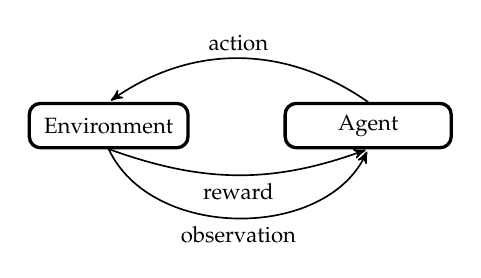
\begin{tikzpicture}[->,>=stealth',shorten >=1pt,auto,node distance=1.5cm,
	semithick, scale = .8, transform shape]
	\node[punkt] (env) {Environment};
	\node[punkt, inner sep=5pt, right=of env] (agent) {Agent};
	\path[->] (agent.north) edge[bend right=35] node[above]{action} (env.north);
	\path[->] (env.south) edge[bend left=-20] node[below]{reward} (agent.south);
	\path[->] (env.south) edge[bend left=-65] node[below]{observation} (agent.south);
	\end{tikzpicture}
	\caption{Interaction between agent and environment in RL}
	\label{fig:agentenvironment}
\end{figure}

When developing RL agents, it is not enough to create algorithm, but also to have a specification of agent environment that allows for a dataflow as described above. The original Deep-Q-Network \cite{mnih_playing_2013} as well as its follow-ups \cite{van_hasselt_deep_2015}\cite{wang_dueling_2015} trained their agents on several \textsc{Atari} games using the \keyword{Arcade Learning Environment} (\textbf{ALE}) \cite{bellemare_arcade_2012}. The ALE was developed with the intention to evaluate the generality of several AI techniques, especially general game playing, reinforcement learning and planning. The important contribution of \cite{bellemare_arcade_2012} was to provide a testbed for any kind of agent, by providing a simple common interface to more than a hundred different tasks. The ALE consists of an Atari-Simulator as well as a game-handling layer, which transformed all of the included Atari-games to a standard reinforcement learning problem. Doing that, it provided the accumulated score so far (corresponding to the reward), the information whether game ended (indicating the end of a training episode), as well as a $160 \times 210$  2D array of 7-bit pixels (corresponding to the agent's observation). As the game screen does not correspond to the internal state of the simulator, the ALE corresponds to a POMDP. The possible input to the simulation consists of 18 discrete actions. 

Environments with discrete actions only are however severly limited, and most of the interesting real-world applications, as for example autonomous driving, require however real-valued action spaces. The test scenarios for the Deep-DPG algorithm consisted thus of a number of simulated physics-tasks, using the MuJoCo physics environment. \\

\noindent Both of the above mentioned environments are by now, among many others, merged into the \keyword{OpenAI gym} environment \cite{brockman_openai_2016}. The OpenAI gym\footnote{\url{https://gym.openai.com}} is created as a toolkit, helping reinforcement learning research by including a collection of benchmark problems with a common interface. The idea is to provide consistent, standardized environments, such that algorithms are easy to benchmark. In that respect, their goal was to provide the reinforcement-learning-pendant of a labeled dataset, such as ImageNet. Aside the previously mentioned ALE as well as a number of physics tasks using the MuJoCo physics-engine, the openAI gym contains the boardgame Go, two-dimensional continous control tasks (\keyword{Box2D games}), a 3D-shooter by the name of \keyword{Doom}, and several other tasks. These tasks are varied in their complexity, input and output: some of them use low-dimensional state representations consisting of only a four-dimensional vector of scalars, while others use a 2D-pixel image of RGB colors.  

The goal of openAI gym is to be as convenient and accessible as possible. For that, one of their design decisions was to make a clear cut between agent and environment, only the latter of which is provided by OpenAI. The exemplary sourcecode found in algorithm \ref{alg:gym}, taken from \url{https://gym.openai.com/docs}, outlines the ease of creating an agent working in the gym framework.
\begin{algorithm}[h]
\lstset{
	numberblanklines=false
	,breaklines=true%
	,tabsize=1%
	,showstringspaces=false%
	,postbreak=\ding{229}\space%
	,escapeinside={*(}{*)}
}
\begin{lstlisting}[language=Python,frame=none]
import gym
env = gym.make('CartPole-v0')
for i_episode in range(20): *($\label{algline:gym_episode}$*)
	observation = env.reset()
	for t in range(100):
		env.render()
		print(observation)
		action = env.action_space.sample()
		observation, reward, done, info = env.step(action)
		if done:
			print("Episode finished after {} timesteps".format(t+1))
			break
\end{lstlisting}%
\caption{Interaction with the openAI gym environment}
\label{alg:gym}
\end{algorithm}
The code outlines how the general dataflow between agent and environment usually takes place: After a reset, the environment provides the first \keyword{observation} to the agent. Afterwards, it is the agent's turn to provide an action. Even though not featured in this easy example, the action is performed by usage of the observation. Once an agent has calculated the action and provided it to the environment, it can perform another simulation step, returning $\langle observation, reward, done, info\rangle$, which is a tuple consisting of another observation of the environment's state, a scalar reward, the information if the episode is finished and it is time to reset the environment, as well as some information for debugging, typically not used in the final description of an agent. In the remainder of this work, I will refer to this dataflow as a baseline on how the interaction of environment and agent should look like.\\

It is worth noting, that the openAI gym is not even 


\section{Self-driving cars}

\subsection{real-life}

Nvidias deep-drive
RRT*
Tesla

\subsubsection{available data in real-life}

Lidar
https://arxiv.org/pdf/1704.03952.pdf


\subsection{games}

Leon wollte hier ne Tabelle von verschiedenen games und den respective inputs die sie nutzen...!


\begin{table}
\resizebox{\textwidth}{!}{
	 \begin{tabular}{c c c c c c}
		Name & Paper/Link & Trained on Game & Used as inputs & Used as reward & Furhter distinctivenesses \\ 
		\hline
		Tensorkart & Link & Mariokart & Y & Z & only pretraining\\
		original DDPG  & \cite{lillicrap_continuous_2015} & Torcs & vision & bla & ne\\
		original DDPG  & \cite{lillicrap_continuous_2015} & Torcs & lowdim & bla & ne\\
		Thatguy & irgendowonmedium & Torcs & vision & besser & ne\\
		NVIDIA & paperlink & real data & vision & bla & ne\\
	\end{tabular}
}
\end{table}

Tensorkart
hier in den fußnoten die ganzen non-scientific quellen wie tensorkart undso

Das Aufteilen von autonomous driving into the subcomponents, wie bei der vorlesung von Julian... oder, as quoted by TORCS-Paper: "The racing problem could be split into a number of different components, including robust control of the vehicle, dynamic and static trajectory planning, car setup, inference and vision, tactical decisions (such as overtaking) and finally overall racing strategy"

DDPG auf torc hat übrigens im pixel-case nen sehrsehr ählnichen punktestand wie im low-dimensional case (1840 vs 1876 im best case, -393 vs -401 im average case).


TORCS!!!!!UNBEDINGT ERWÄHNEN DASS die geschreiben haben dass TORCS ein POMDP ist!!
	\chapter{Program Architecture}

\label{ch:program}

The program was written by the author of this work and is licensed under the GNU General Public License (GNU GPLv3). Its source code is attached in the appendix of this work and additionally can be found digitally on the enclosed CD-ROM. The machine learning part was written in \textsc{Python}, using the \textsc{Tensorflow}-library \parencite{abadi_tensorflow:_2015}.
%TODO: TF-version, dann noch was zu Unity!!!

[tf gibt automatic differentiation, multi-gpu support, python interface]

\section{Design choices}
%\begin{algorithm}[H]
%	\KwData{this text}
%	\KwResult{how to write algorithm with \LaTeX2e }
%	initialization\;
%	\While{not at end of this document}{
%		read current\;
%		\eIf{understand}{
%			go to next section\;
%			current section becomes this one\;
%		}{
%		go back to the beginning of current section\;
%	}
%}
%\caption{How to write algorithms}
%\end{algorithm}

\subsection{The game as a reinforcement learning problem}

-ungefähres UML-diagramm
-das spiel itself ist ein partially observable MDP, und es ist (as tested) surprisingly indeterministic

[Ah. Should have googled first before posting. Differences in FPU calculations on different processors. Differences in timing affecting things like the number of times a random number generator is called. These can cause the physics to get out of sync]
https://forum.unity3d.com/threads/is-unity-physics-is-deterministic.429778/

\subsection{The vectors}

\subsection{Exploration}

\subsection{Reward}

\subsection{Performance measure}

\section{Implementation}

\subsection{The game}

\subsubsection{What Leon did already}

\subsubsection{Communication}

-den sockets post
-das von leon gemalte ablaufdiagramm

\subsection{The agent}

Unbedingt auf jeden Fall UML-diagramm

\subsubsection{Challenges and Solutions}

DQN vs DDPG, sehend vs nicht-sehend, ...

\subsubsection{Pretraining}

\subsubsection{The different agents}

sehend vs nicht sehend, ...

\subsubsection{Network architecture}

1. dqn-algorithm
- anzahl layer, Batchnorm, doubles dueling
- clipping wieder rein, reference auf das dueling
- grundsätzlich gegen batchnorm entschieden, siehe reddit post
- MIT GRAFIK
- Adam und tensorflow quoten, siehe zotero
2. ddpg
- anzahl layer, Batchnorm
- MIT GRAFIK

-schöne grafik.
-auf meien DQN-config eingehen und(!!!) ne DDPG-config machen, using the "experiment details" vom ddpg paper  


In the original DDPG-algorithm \cite{lillicrap_continuous_2015}, the authors used \keyword{batch normalization} \cite{ioffe_batch_2015} to have the possibility of using the same network hyperparameters for differently scaled input-values. In the learning step when using minibatches, \batchnorm normalizes each dimension across the samples in a batch to have unit mean and variance, whilst keeping a running mean and variance to normalize in non-learning steps. In Tensorflow, batchnorm can be added with an additional layer and an additional input, specifying the phase (learning step/non-learning step)\footnote{cf. \url{https://www.tensorflow.org/api\_docs/python/tf/contrib/layers/batch_norm}}. Though Lillicrap et al. seemed to have success on using \batchnorm, in practice it lead to unstability, even on simple physics tasks in openAI's gym. As I am not the only one having this issue \footnote{redditlink}, I left out batch normalization for good.

 
	\chapter{Results -- Implementation}

\label{ch:implementationresults}

This chapter provides the implementation of the \term{features} of the implemented agents. It will start with the \term{possible vectors} that are sent to any agent and can be used. Afterwards, the agents that where implemented in the scope of this thesis are explained, including all their features and why they were selected this way. These features include the used \codeobj{model}s, the exploration-functions, their specific observation-functions (using the \term{possible features}), their methods of incorporating pretraining as well as their reward-functions. 

It is worth to note, that some of these functions (as for example the \codefunc{calculateReward(gameState)} function) are implemented not in the individual agent, but in \codeobj{AbstractRLAgent}, as they would otherwise have to be redundantly implemented multiple times.

%############################################################################################
\section{Possible vectors}
%############################################################################################

\label{ch:thevectors}

%-progressvec (progress, laptime, lapcount, validvec)
%-speedsteer (motortorques, steerangle, velocity, fRightDirection, velocity of perpendiculars, angle, speedinstreetdir, speedintraversedir, cuvinessbeforecar)
%-carstatusvec (longitutinal and latidutialn slip for each tire)
%-centerdist, als vector
%-waldistvec (direction the car faces, steers, moves..... and directiont the street goes (each longsighted and shortsighted from car and streetmiddle)
%-lookahead-vector
%-delta und feedback
%-actual action (possibly overwritten)
%-both vision-vectors

\term{Possible Vectors} refers to all information the game streams over its socket to the agent. While most of this information will be used to make up an agent's state, the vectors also provide information about if the game must be reset as well as information to calculate the reward from. This information is collected in Unity in the function \codefunc{GetAllInfos()}, and converted into a namedtuple-wrapper called \codeobj{Otherinputs}, specified in \filename{read\_supervised.py}. In this section, I provide an overview of those vectors and their meaning in the game. I refer to the individual possible vectors by the name used in \codeobj{Otherinputs}.

\paragraph{ProgressVec} This vector contains information about the current progress of the car on the track, which consists of the actual progress in percent, the time the car needed for the current lap so far, the number of the current lap, as well as the flag if the round is still \keyword{valid}.

\paragraph{SpeedSteer} In this vector, information about the car's velocity and its steer angle is encoded. It consists of the following values:

\renewcommand{\arraystretch}{1.3}
\begin{flushleft}
	\begin{tabular}{>{\em}p{2.9cm} p{\textwidth-3.8cm}} 
		RLTorque & The motor torque applied to the left back tire\\
		RRTorque & The motor torque applied to the right back tire\\
		FLSteer & The steering angle of the front left tire\\
		FRSteer & The steering angle of the front right tire\\
		velocity & The velocity of the car as scalar independent of directions\\
		rightDirection & A boolean value if the car moves into the intended direction\\
		velocityOfPerpendicular & \hspace*{0.8cm} The velocity of the orthogonal projection of the car onto the center of the street\\ %TODO see sectionbalabla, wo ich DOCH die definition von perpendicular einführen werde
		carAngle & The car's angle (in degrees) in relation to the street's direction\\
		speedInStreetDir & The car's velocity into the street's direction (calculated using the dot-product between the car's velocity-vectors and the direction-vector of the street at the car's current position)\\
		speedInTraverDir &  The car's velocity into the orthogonal of the street's direction\\
		CurvinessBeforeCar & A measure of the curvature of the street immediately ahead of the car ($CurvinessBeforeCar \in [0,1]$, where a value of zero corresponds to a straight street)\\	
	\end{tabular}
\end{flushleft}

\paragraph{StatusVector} This vector contains eight values, corresponding to the forward slip and sideways slip of each of the car's tires, using a function provided by Unity's \codeobj{WheelCollider}-object. The more the car slips, the smaller the impact of movement commands. The current slip-values are presented in the GUI of the game (and can be seen behind annotation \textbf{R} in figure~\ref{fig:aidriveshot}).

\paragraph{CenterDist and CenterDistVec} The \emph{CenterDist} corresponds to the car's orthogonal distance to the street's center in the form of the \keyword{perpendicular} (also visually represented in the car's GUI, behind annotation \textbf{N} in figure~\ref{fig:aidriveshot}).
The \emph{CenterDistVec} contains the same information presented in another way: It is a vector of length 15, where the middle element corresponds to the car's longitutional position. The other elemnts correspond to points with regular distances to the car's left and right. The value of each respective element is calculated using the reversed distance between this position and the longitudional center of the street. The content of this vector is visually represented behind annotation \textbf{M} in figure~\ref{fig:aidriveshot}.

\paragraph{WallDistVec} This vector contains seven values, corresponding to the car's distance to the wall along a certain ray. It does not contain the closest distance to the wall -- because this value is already represented by the CenterDist. As the wall has always a fixed distance from the street's center (with an absolute value of five), the distance to the closest wall can be calculated as $5 - abs(CenterDist)$. 
For the calculation of the \emph{WallDistVec}, several rays are casted from the car's (or the perpendicular's) position into a particular direction. Returned is then the distance from their respective origin and their first intersection with a wall. The vector contains seven values, using rays with different origins and different directions. In the following table, I provide an explanation of each of those values, while figure~\ref{fig:walldistvec} in appendix~\ref{AppendixB} visually represents these rays. The respective color is mentioned in the table.
\renewcommand{\arraystretch}{1.3}
\begin{flushleft}
	\begin{tabular}{p{0.5cm} p{2cm} p{2.4cm} p{\textwidth-6.45cm}} 
		\# & color in \ref{fig:walldistvec} & origin & direction \\
		\hline
		1 & \textcolor{black}{black} & car's center & direction the car faces \\
		2 & \textcolor{magenta}{magenta} & car's center & direction the car steers\\	
		3 & \textcolor{red}{red} & car's center & direction the car moves\\	
		4 & \textcolor{black}{white} & car's center & short-sighted direction of the street (calculated as the vector between the closest \codeobj{anchorVector} behind the car and the closest one before the car) \\		
		5 & \textcolor{yellow}{yellow} & perpendicular & short-sighted direction of the street (calculated as the vector between the closest \codeobj{anchorVector} behind the car and the closest one before the car) \\
		6 & \textcolor{blue}{blue} & car's center & long-sighted direction of the street (calculated as the vector between the closest \codeobj{anchorVector}  to the car and the one 5 in advance) \\
		7 & \textcolor{gray}{gray} & perpendicular & long-sighted direction of the street (calculated as the vector between the closest \codeobj{anchorVector}  to the car and the one 5 in advance) \\
	\end{tabular}
\end{flushleft}

\paragraph{LookAheadVec} This vector corresponds to the course of the street ahead of the car. It is a 30-dimensional vector, corresponding to regularly spaced \codeobj{anchorVector}s, starting at the position of the car, following the direction of the street. The value at each position $i$ of this vector corresponds to the angle between the direction of the street at position $i$ and the direction at position $i+1$. In other words, if the street makes a shart turn 4 units ahead of the car, then element $3$ will contain a high value. The angle is measured in degrees. A graphical representation of this vector can be seen behind annotation \textbf{N} in figure~\ref{fig:aidriveshot}.

\paragraph{FBDelta} This vector consists of two values, namely \emph{Feedback} and \emph{Delta}. The Feedback-value is the temporal difference of how long the car needed for a specific section of the course (constrained via the a \codeobj{anchorVector} close to the car) in the current process in comparison to the time needed in the fastest lap so far. The Delta-value is the absolute difference in time needed for the entire lap so far.

As both of these values are only useful in relation to the time needed for the fastest lap, it must be ensured that this does not change during training. For that, The file \filename{AiInterface.cs} contains in its class \codeobj{Consts} a flag \codeobj{lock\_fastestlap\_in\_AIMode}. Note however, that even if this flag is set, the values of \emph{FBDelta} could at most be used to calculate the agent's reward and not as part of its state.

\paragraph{Action} This is a three-dimensional vector corresponding to the actual action the environment recorded. While the agent knows what action it provided, it could be manually overwritten (after the press of \keystroke{H}) -- which is why the agent stores this vector in its replay memory instead of the action it would have performed otherwise.


\paragraph{minimaps} While the minimaps are not contained in the namedtuple \codeobj{Otherinputs}, their value is transmitted from the game just like the other vectors. In the current implementation, both cameras have a resolution of $30\times45$ pixels, where one camera is $15$ units away of the car, and the other one $75$ units, which means that the former provides a smaller but more detailed view of the car. The closer camera is mostly referred to as $vvec2$, whereas the other one is denoted $visionvec$ or $vvec$.\\

As a working game was already provided by \leon of this thesis, so were some of these vectors, namely the calculation of FBDelta, LookAheadVec, CenterDist and CenterDistVec.

It is worth noting that most \term{possible vectors} are normalized after loading, according to (in part estimated) minimal- and maximal values, such that all their values in [0,1]. The corresponding \codeobj{MINVALS} and \codeobj{MAXVALS} are defined in \filename{read\_supervised.py}

%############################################################################################
\section{Implemented models}
%############################################################################################

Within the context of this thesis, two different models were developed that can be used for agents to learn and play the given game: a \keyword{Double Dueling Deep-Q-Learning} model, specified in the class \codeobj{DDDQN\_model} in \filename{models/dddqn.py}\footnote{\url{https://github.com/cstenkamp/BA-rAIce-ANN/blob/master/models/dddqn.py}} as well as a \keyword{Deep Deterministic Policy Gradient} model, specified in \codeobj{DDPG\_model} in \filename{models/ddpg.py}\footnote{\url{https://github.com/cstenkamp/BA-rAIce-ANN/blob/master/models/ddpg.py}} The theory of the model was explained in chapters~\ref{ch:DQN}ff and \ref{ch:ddpg}, respectively. 

Both models can take two-dimensional as well as one-dimensional input and return outputs corresponding to the action that needs to be taken, which are three real numbers. One has to be aware though that while a DDPG-model can naturally return such, a DQN-model only works for discrete actions. Because it was developed with DQN-models in mind, the \codeobj{AbstractAgent} contains functions to \codefunc{discretize} the action-value returned by the game to a one-hot vector to be used by the model, as well as functions to \codefunc{dediscretize} a one-hot vector from the model that can be used by the environment. It is obvious, that discretizing actions has severe disadvantages: If the discretization is very fine-grained, the action-space becomes intractably big due to a combinatorial explosion (the \textit{curse of dimensionality}), whereas if a discretization is coarse, much of the information is lost and precise steering becomes impossible. A further downside of discretizing actions into one-hot vectors is, that it limits the design space of exploration strategies, as information about similiarity of actions is lost and only the uninformed $\epsilon$-greedy mechanism remains possible.



\noindent While the learning technique differs in both implemented models, both implement the interface provided in figure~\ref{fig:modelsInt}, such that the functions relevant for the agent are accessible in the same way. An UML-diagram of most of the agent's functions as well as the interface is given in figure~\ref{fig:modelssmall}. If an agent does not need to discretize actions, it must overwrite the method \codefunc{getAction(gameState)}.

\begin{figure}[h]
	\centering 
	\includegraphics[width=\textwidth]{uml_diagrams/models_inText2.2}
	\caption[UML-diagram of the two models and their interface]{UML-diagram of the two given models as well as the interface both of them implement}
	\label{fig:modelssmall}
\end{figure}

Both implemented models provide the possibility to load and save a model from/to the harddisk using TensorFlow's saver-class. If a model is loaded in the \codeother{isPretrain}-mode, it can be saved to file and loaded again such that it is usable. If the model is saved, the information about its already performed numbers of inferences and learning-steps are saved within TensorFlow as well. When a model is saved, it saves into the directory \codeobj{conf.pretrain\_checkpoint\_dir} if the respective flag is set, and \codeobj{conf.checkpoint\_dir} otherwise. When loading a model (in \codefunc{initNet(load)}), the \codefunc{load}-parameter specifies if the model should be loaded from the pretrain-directory, the non-pretrain-directory or none at all.


While both models are implemented to be used by an agent as described above and in the described situation, they are general models for reinforcement learning -- and are as such usable to learn reasonable policies in any task described as Markov decision process. To show the generality of the implemented models, a file \filename{gym\_test.py}\footnote{\url{https://github.com/cstenkamp/BA-rAIce-ANN/blob/master/gym\_test.py}} is provided. In this file, the implemented \codeobj{model}s are used to solve arbitrary \term{OpenAI-gym}-tasks. As the program flow of the interaction with a gym-environment differs to that one of the implemented program, the file contains specialized definitions of \codeobj{agent}, \codeobj{config} and \codeobj{memory} to work with the API-schema of \term{gym}. As \term{gym}-environments explicitly define \codeobj{terminal} and \codeobj{reward}, the \codeobj{agent} must for example not work with the \codeobj{gameState}, but contains only methods using the immediate \codeobj{agentState}. The way how an agent accesses its model is however equal to the agents for the given game. The \filename{gym\_test.py} can be used to test if a model is functional -- if a model works on several gym-tasks, it can be assumed that it is implemented correctly. Having such a method at hand is very handy during the implementation of reinforcement-learning agents, as it provides a reliable method to check where the reason for any errors may lie. Both implemented models were successfully tested on several tasks each\footnote{Note however, that using other gym-environments than the ones on which was tested (\codeobjFN{Pendulum-v0}, \codeobjFN{FrozenLake-v0}, \codeobjFN{MountainCar-v0} and \codeobjFN{CarRacing-v0}) may require implementing specific exploration or preprocessing techniques. Note further, that some environments can only be solved with models that allow for continuous action-spaces.}.


In the following two sections, I will at first explain the DQN-model and afterwards the DDPG-model. Note that both models are used in multiple agents each. The amount of input-values may differ from agent to agent, and the presented network architecture is specific to one of the implemented agents as stated.


\subsection{DQN-model}

In the \term{Drive}-mode of the game, throttle and steering are both binary, but it is still possible for Users to drive the course well. Because of that, it was decided to keep steering and throttle binary for this model as well to reduce the dimensionality of discretization. Further, simultaneous activation of throttle and brake was forbidden. Because of these design choices, an action for a DQN-model is a one-hot vector of the size \codeobj{3*conf.steering\_steps}, with steering\_steps set to 7 in the current version. 

The class \codeobj{DDDQN\_model} \term{has} two \codeobj{DuelDQN}s, which are Deep Convolutional Neural Networks with Dueling Architectures, specified as computational graph using TensorFlow -- one of them being its online network, and the other the target network. The \codeobj{DDDQN\_model} combines them for the learning method of Double-Q-Learning (as detailed in section~\ref{ch:DQN}ff as well as appendix~\ref{AppendixA}) in its method \codefunc{q\_train\_step}. 

The provided DQN-model can however not only learn via Q-learning, but can also be trained supervisedly. For that, it specifies the function \codefunc{sv\_train\_step}. This method can only be called if \codeobj{isPretrain} and learns directly on its target network. For that, the used \codeobj{DuelDQN}s must provide a TensorFlow-placeholder for the target-action. An agent that pretrained supervisedly however should not subsequently be used for reinforcement learning (an explanation for that will follow in section~\ref{sec:resultsupervised}).

It was mentioned before that the model incorporates hard-coded domain-specific knowledge. Next to the ban of simultaneous braking and steering as action, the model explicitly forbids actions that do not accelerate the car if it is standing. As already mentioned, part of the \codeobj{agentState} is a \codeobj{stands\_input}, which the method \codefunc{getAgentState} sets to \codeobj{true} if the car's velocity is below a certain value. The model consistently has a \codeobj{stands\_input} expecting such a boolean value. Note that the model's \codefunc{make\_inputs} also actively sets this value to \codeobj{true} if the car stood up to a specified number of inferences before the current one. If this value and the respective option \codeobj{conf.use\_settozero} are both \codeobj{true}, then the model sets in its function \codefunc{settozero} all Q-values of actions that do not include accelerating the car to zero. As a DQN-based model selects its actions using a \textit{greedy} strategy, it always selects the action with the highest Q-value -- which is now the maximum of all Q-values that include the action of accelerating the car. Note however, that the model's \codeobj{stands\_input} is only set to \codeobj{true} in inferences, and not in learning-steps.

The network architecture of the two \codeobj{DuelDQN}s that the agent uses is described in the next section. Note that a \codeobj{DuelDQN} is a particular class \term{know}n to the agent. All TensorFlow-Layers, inputs, outputs as well as a \codeobj{saver} and certain collections can be accessed from the \codeobj{DDDQN\_model}. As explained in chapter~\ref{ch:DQN}, the use of both online-network to train on as well as target-network to sample experiences from is necessary for adequate performance. As suggested by \cite{lillicrap_continuous_2015}, the implementation of this DQN uses \textit{soft target-updates}, meaning that after every \codefunc{q\_train\_step} the relevant weights of the target-network are moved by a factor $0 < \tau \ll 1$ into the direction of the online-network. To do so, both networks maintain a collection of their trainable variables,  \codeobj{trainables}. The respective assignment operations are added to the computational graph as \codeobj{smoothTargetNetUpdate}, specified in the model's \codefunc{\_\_init\_\_}. After initializing a model or loading it from a file, a similar assignment operation is performed to ensure that both networks are equal.

\subsubsection{Network architecture}

An overview of the general network architecture, as used by the \term{dqn\_rl\_agent}, is provided in figure~\ref{fig:dqn_graph}. Note however that the actual architecture differs in other agents, as it depends on the agent's configuration of \term{features}. As some agents do not use the minimaps as input, their implementation for those does not use any of the convolutional layers from the upper line of the figure. When initializing a \codeobj{DuelDQN}, a reference to the agent is passed, such that the network knows how many input and output-neurons to specifiy.

\begin{figure}[h]
	\centering 
	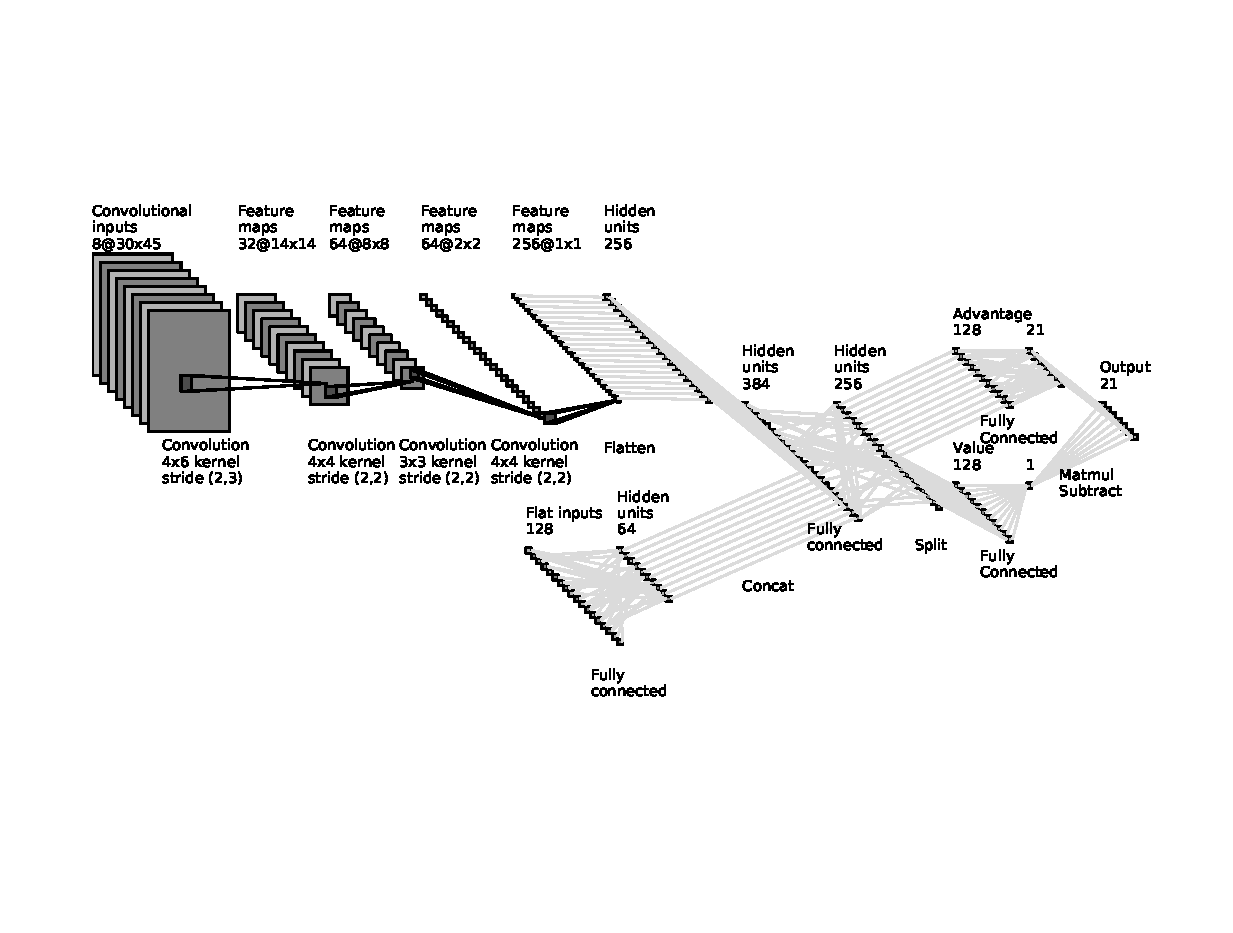
\includegraphics[trim={1.22cm 3.4cm 1.15cm 3cm},clip,width=1.02\textwidth]{draw_convnet/dqn}
	\caption{The used convolutional DQN with a dueling architecture}
	\label{fig:dqn_graph}
\end{figure}

If convolutional input is specified, four convolutional layers layers process the input to 256 feature-maps of size $1 \times 1$, which can subsequently be flattened to a one-dimensional layer. Note that there are no pooling layers in between convolutional layers. As suggested by \cite{springenberg_striving_2014}, pooling leads to a loss of localization information and can be discarded in favor of a larger \term{stride} in the convolutional layers.

\noindent While the two-dimensional \codeobj{conv\_inputs} are processed with convolutional layers, \codeobj{ff\_inputs} are fully connected to a hidden layer of variable size. This layer is concatenated to the flattened output to the convolutional layer, the result of which is densely connected to another hidden layer of 256 neurons. This layer is then, following the dueling architecture from \cite{wang_dueling_2015}, split into a separate \keyword{advantage stream} and \keyword{value stream}. While the value stream is fully connected to one hidden layer (corresponding to the state-value), the advantage ends in one output neuron for each action, which is 21 in the current implementation. The advantage stream and value stream are finally combined (as described in section~\ref{sec:dueling}) to yield 21 output neurons, corresponding to one Q-value for every action in the provided state.

Informal search led to the selection of the rectified non-linearity (\codeobj{tf.nn.relu}) as activation function as well as Adam\cite{kingma_adam:_2014} as optimizer. All weights of this network are initialized around zero (or slightly higher, to prevent \keyword{dead neurons} in combination with the relu activation-function) with only a very small standard deviation ($10^{-20}$ up to $10^{-3}$), as doing otherwise showed to impair the agent's performance after a fresh start.

In the current implementation, the DQN-model does not perform \keyword{batch normalization}\cite{ioffe_batch_2015}, as it showed to impair the agent's performance. The functions \codefunc{convolutional\_layer} and \codefunc{dense}, which are used to initialize the layers, wrap respective TensorFlow-functions and can be found in \filename{utils.py}\footnote{\url{https://github.com/cstenkamp/BA-rAIce-ANN/blob/master/utils.py}}.

The final structure of this network was subject of much experimentation. Any used hyperparameter that does not correspond to its counterpart in \cite{mnih_human-level_2015} or \cite{wang_dueling_2015} is the result of informal search, showing the best performance so far. This does by any means not mean that the parameters are optimal. Using this structure, the network performed reasonably well on given OpenAI gym-tasks, as explained earlier in this chapter.


\subsection{DDPG-model}

A DDPG-model must incorportate four ANNs to work correctly: an online- and a target version of both \codeobj{actor} and \codeobj{critic}, as found by \cite{lillicrap_continuous_2015}.  While the online networks will be used for online predictions and will be updated at every timestep, the target networks will be used for determining the directions into which the online networks should be updated. The given implementation of the \codeobj{DDPG\_model} thus \term{has} an actor and a critic, which in turn have two \codeobj{actorNet}s or \codeobj{criticNet}s, respectively. If the \codefunc{save()}-method of \codeobj{DDPG\_model} is called, it calls the respective functions of actor and critic, which save their individual variables individually. Because of that, the same critic could be used for different actors or vice versa. The information about the numbers of current inferences and others is saved in and loaded from the actor.

As the \codeobj{DDPG\_model} \term{has} \codeobj{actor} and \codeobj{critic}, it can access all their values and methods. If it accesses any of these, it specifies as argument if it wants them to internally use their online- or target network. Both actor and critic provide respective methods to update their target network.

It is not possible to use the same network structure as used in the \codeobj{DQN\_model} in any network of the \codeobj{DDPG\_model}. The actor returns continuous values which correspond directly to the action instead of a \term{softmax}-distribution over possible discrete actions. The critic needs, in contrast to the DQN-architecture, the actions as additional input to return one single Q-value. It is obvious that the \term{dueling architecture} cannot be adopted for the DDPG-critic.

In its \codefunc{q\_train\_step}-method, the \codeobj{DDPG\_model} trains both its actor and its critic by calling their respective methods -- the theoretical basis of this learning step is explained in section~\ref{ch:ddpg}, while appendix~\ref{ap:ddpg} compares the source-code to the pseudocode given in \cite{lillicrap_continuous_2015}. While normally TensorFlow minimizes losses via an optimizer (and also does so in the critic), it also allows the possibility to \codefunc{apply\_gradients}, which optimizes all elements of its respective computation graph into the direction of the supplied values. 

As the actor only needs the critic's gradients once, these can simply be passed into its \codeobj{feed\_dict}. Besides this interaction, actor and critic can be implemented completely independent of each other. In the following section, The network structure of both of them will be described individually. It is worth noting, that this model supports the usage of \keyword{TensorBoard}, and saves a summary of all its variables in a preset interval of update-steps.

\subsubsection{Network architecture}

\paragraph{Critic}

The actual computational graph of the network the \codeobj{critic} uses is specified in an extra class. In contrast to the \codeobj{DQN\_model}, it was decided to use a different class for agents that use convolutional input than for agents which do not, as informal testing showed that the \codeobj{DDPG\_model} appears to be less forgiving to changes of its network structure. This means, that the \codeobj{critic} uses a \codeobj{conv\_criticNet} if \codeobj{agent.usesConv} and a \codeobj{lowdim\_criticNet} otherwise.

In contrast to the model of a DQN, the critic gets a state and an action as input, returning a single estimate of the respective state-action value \term{Q}. Like a DQN however, it is trained using temporal differences, requiring a better estimate of each Q-value to update its parameters. As however only the online network is updated this way (whereas the target-network receives smooth updates), the \codeobj{placeholder} to hold these is specified in the class \codeobj{Critic}, not in one of its used networks. The \codeobj{Critic}-class further specifies a function to return the \codefunc{action_gradiens(inputs, actions)} for the \codeobj{actor}.

The network-architecture of the convolutional critic is specified in figure~\ref{fig:2dcrit}. 

\begin{figure}[h]
	\centering 
	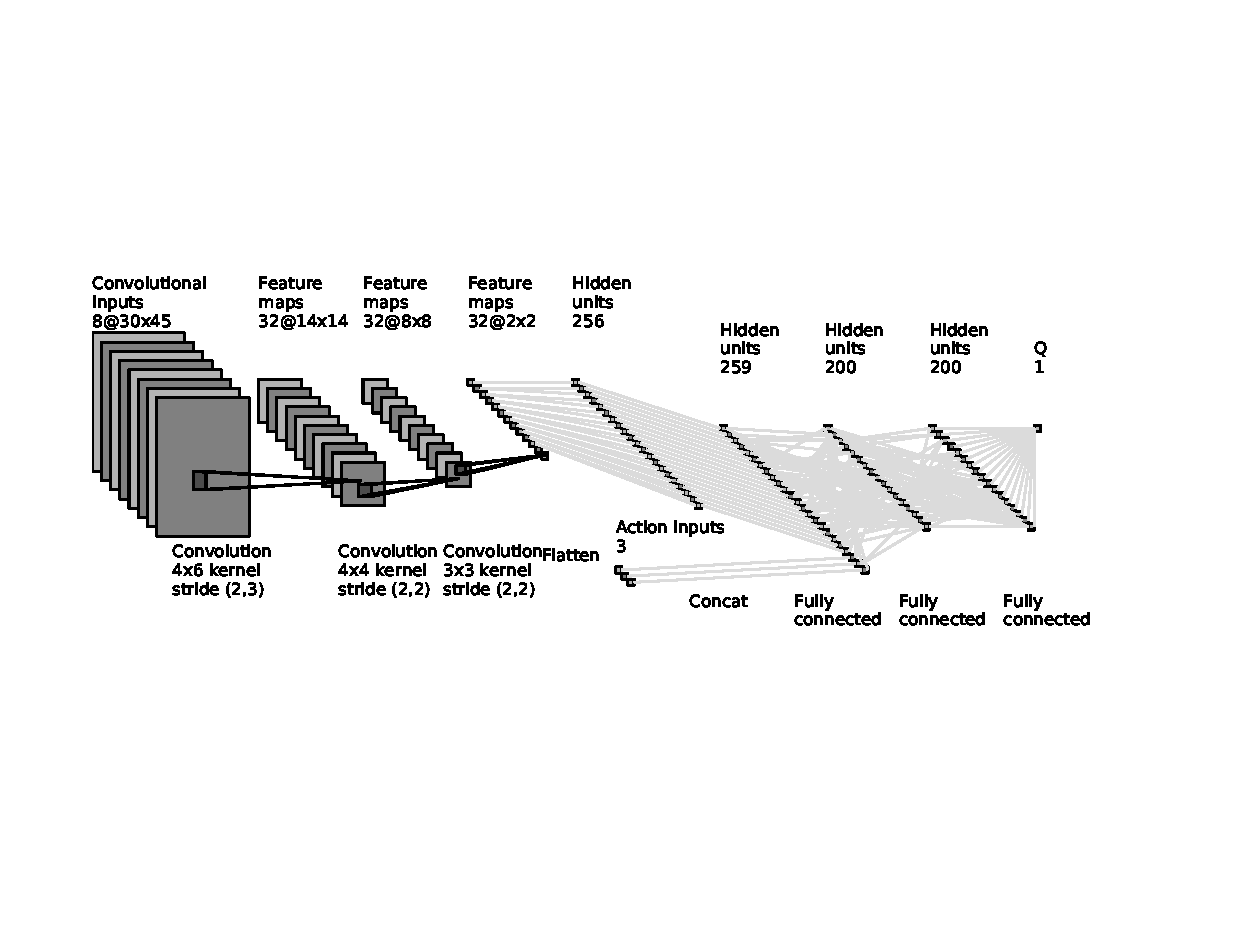
\includegraphics[trim={1.22cm 4.6cm 2cm 3cm},clip,width=1.05\textwidth]{draw_convnet/critic-2d}
	\caption{Convolutional critic}
	\label{fig:2dcrit}
\end{figure}

The number of input-maps is variable, however the kernel size and stride of the convolutional layers are adjusted for an input-size of $30\times45$ pixels to create 32 $2\times2$ feature maps in three convolutional layers (again, pooling layers were dropped in favor of higher stride).  Afterwards, the feature maps are flattened into a layer of 256 hidden units, to which the 3 action-inputs are concatenated. This layer is densely connected to two other hidden layers of 200 units, which ultimately leads to one output-neuron: the Q-value.\\

\noindent The network-architecture of the low-dimensional critic (\codeobj{lowdim\_criticNet}) is depicted in figure~\ref{fig:lowdcrit}.

\begin{figure}[h]
	\centering 
	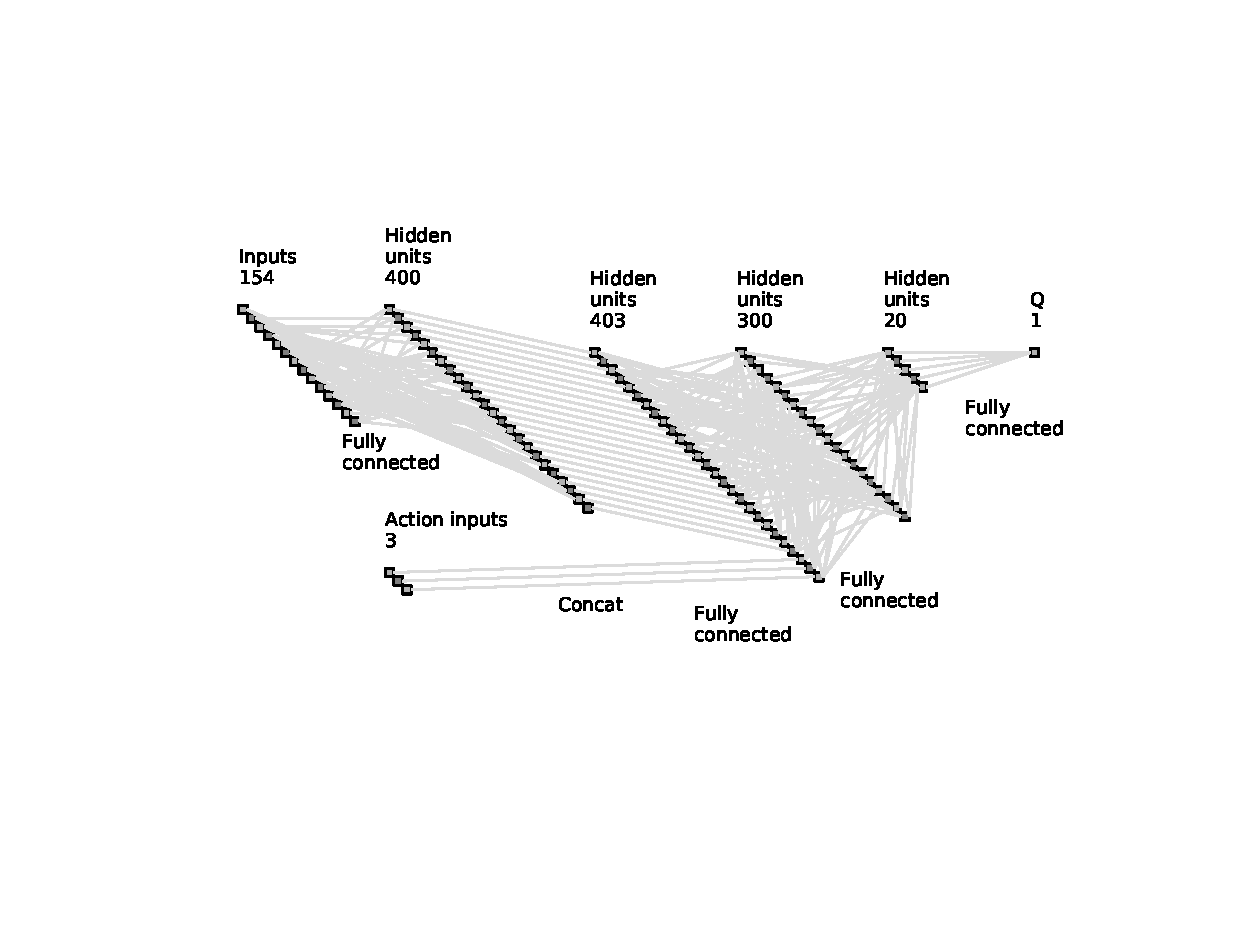
\includegraphics[trim={3.7cm 4.4cm 2cm 3cm},clip,width=.98\textwidth]{draw_convnet/critic-lowd}
	\caption{Low-dimensional critic}
	\label{fig:lowdcrit}
\end{figure}

The number of input-neurons the low-dimensional critic uses is variable depending on the agent -- for the \filename{ddpg\_novison\_rl\_agent} it consisted of 154 inputs. These are densely connected to a layer of 400 hidden units, to which the 3 action-inputs are concatenated. This layer of 403 units is fully connected to another hidden layer of 300 units, which is connected to a layer of 20 hidden units. This final hidden layer is connected to the output-layer specifiying the Q-value.

As suggested by \cite{lillicrap_continuous_2015}, both variants of the critic use $L2$ weight decay for all their layers. Furthermore, the implementation allows to use \keyword{batch normalization}\cite{ioffe_batch_2015}, which can be toggled for each layer individually with a respective argument. In the original DDPG-algorithm, the authors used this technique in order to use the same network hyperparameters for differently scaled input-values. In the learning step when using minibatches, \batchnorm normalizes each dimension across the samples in a batch to have unit mean and variance, whilst keeping a running mean and variance to normalize in non-learning steps. In Tensorflow, batchnorm can be added with respective additional layers and one additional input that specifies the phase (learning step/non-learning step)\footnote{for further information, see \url{https://www.tensorflow.org/api\_docs/python/tf/contrib/layers/batch_norm} [accessed on 5th September, 2017]}. Though \cite{lillicrap_continuous_2015} report success on using batch normalization, in practice it often leads to instability. After much informal it turned out that using \batchnorm in the critic only harms the performance by giving a very small and similar Q-value for all states, which is why it is deactivated in the final implementation.

\noindent All layers are summarized with the function \codefunc{variable\_summary} from \filename{utils.py}, writing their summary to a file that can be inspected by \term{TensorBoard} every \codeobj{conf.summarize\_tensorboard\_allstep} steps. 


\paragraph{Actor}

Just like the \codeobj{critic}, the \codeobj{actor} uses a \codeobj{conv\_actorNet} if \codeobj{agent.usesConv} and a\\ \codeobj{lowdim\_actorNet} otherwise.

The network architecture of the high-dimensional critic can be inspected in figure~\ref{fig:2dact}. Its structure is similar to that of the high-dimensional critic, with the difference that the actor does not take the actions as input, but connects the last hidden layer to three output neurons, corresponding to the values for the three actions. This \keyword{Outs}-layer is scaled afterwards to yield the \keyword{ScaledOuts}-layer. All hidden units but the last use a \codeobj{tf.nn.relu} activation function, whereas the last uses a \codeobj{tanh}-activation-function. While $tanh$ has a range of $[-1,1]$, the actions may have a different range (e.g. $acceleration \in [0,1]$). The final scaling layer adjusts the range correspondingly.

\begin{figure}[h]
	\centering 
	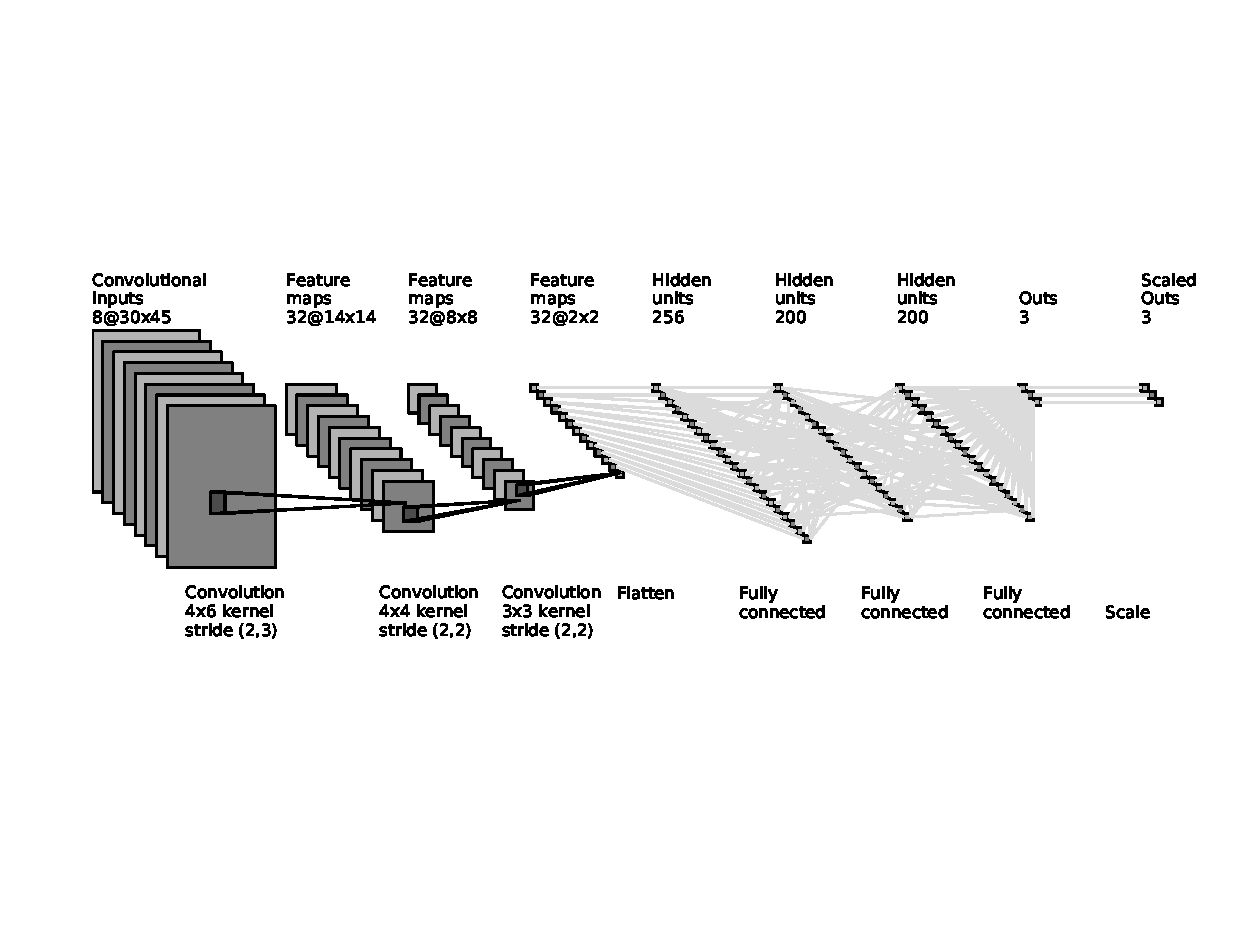
\includegraphics[trim={1.22cm 5.03cm 0.4cm 3cm},clip,width=1.01\textwidth]{draw_convnet/actor-2d}
	\caption{Convolutional actor}
	\label{fig:2dact}
\end{figure}

The structure of the low-dimensional actor (figure~\ref{fig:lowdact}) is fairly simple. The inputs are fully connected to 300 hidden units, which are fully connected to another 200 hidden units, which is in turn connected to the output-units, which are scaled again as in the convolutional case. 

\begin{figure}[h]
	\centering 
	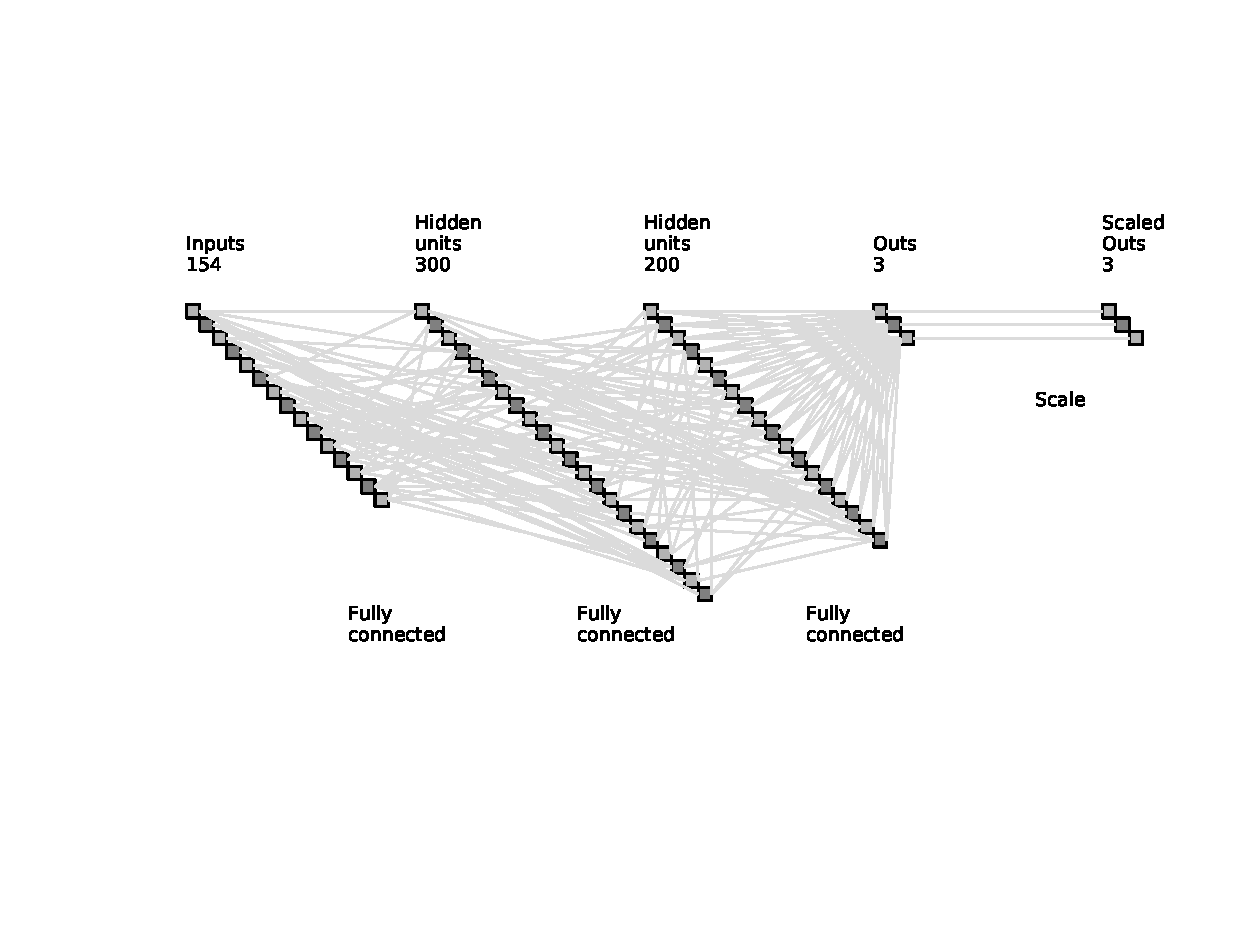
\includegraphics[trim={2.7cm 4.2cm 0.8cm 3cm},clip,width=1.01\textwidth]{draw_convnet/actor-lowd}
	\caption{Low-dimensional actor}
	\label{fig:lowdact}
\end{figure}

In contrast to the critic, the actor does not use $L2$ normalization, as suggested by \cite{lillicrap_continuous_2015}. Informal testing showed, that \batchnorm indeed helps convergence in the actor, which is why it is enabled for all fully-connected layers. Besides the critic's preterminal layer, all hyperparameters correspond roughly to \cite{lillicrap_continuous_2015}, with all differences being the result of informal testing. As in the DQN-model, the rectified non-linearity (\codeobj{tf.nn.relu}) serves as activation function and Adam\cite{kingma_adam:_2014} as optimizer. The convolutional layers are implemented using \codeobj{conv2d} from TensorFlow's \codeobj{slim} package. All layers that are recorded for TensorBoard are added to the collection \codeobj{summaryOps}.

Like the DQN-model, this model also incorporates a function that forces the model to accelerate if the \codeobj{stands\_input} is set to \codeobj{true}. This is however implemented differently, as it is not necessary to change the Q-value of actions because the output of the actor can be changed instead. If the corresponding variables \codeobj{conf.use\_settozero} and \codeobj{stands\_input} are \codeobj{true}, the value for the $brake$ is simply set to zero, whereas the value for $throttle$ is set to a random value of at least $0.5$. 

Further, the DDPG-model also manually forbids simultaneous braking and accelerating. In contrast to the DQN-model however, no combined action is returned, but an individual value for $throttle$ and $break$. In the method \codefunc{apply\_constraints}, the actor checks if both values are simultaneously above $0.5$, and randomly sets one of those to a random value below $0.5$ if so.

Agents that use the DDPG-model must overwrite the functions \codefunc{makeNetUsableAction} to account for the fact the DDPG-model works with un-discretized action and needs these as input to perform its learning step. 
It was further mentioned in section~\ref{sec:contexptheory} that an agent using a continuous model works better with noisy actions instead of completely random actions as exploration function. To do so, a method like \codefunc{make\_noisy}, and the change the implemented \codefunc{randomAction(gameState)} are required.

%############################################################################################
\section{Implemented agents}
%############################################################################################

In the course of this thesis, five different agents were implemented to both demonstrate how to use the given framework and answer the research questions stated in section~\ref{sec:researchquestions}.  The following table shows their names and distinctive properties: 

\begin{flushleft}
\begin{tabular}{l l l l}
	filename & uses model & uses visionvector & performs RL\\
	\hline
	\textbf{ddpg\_novision\_rl\_agent}.py\footnote{\url{https://github.com/cstenkamp/BA-rAIce-ANN/blob/master/agents/ddpg_novision_rl_agent.py}} & DDPG & no & yes\\	
	\textbf{ddpg\_rl\_agent}.py\footnote{\url{https://github.com/cstenkamp/BA-rAIce-ANN/blob/master/agents/ddpg_rl_agent.py}} & DDPG & yes & yes\\
	\textbf{dqn\_novision\_rl\_agent}.py\footnote{\url{https://github.com/cstenkamp/BA-rAIce-ANN/blob/master/agents/dqn_novision_rl_agent.py}} & DQN & no & yes\\
	\textbf{dqn\_rl\_agent}.py\footnote{\url{https://github.com/cstenkamp/BA-rAIce-ANN/blob/master/agents/dqn_rl_agent.py}} & DQN & yes & yes\\
	\textbf{dqn\_sv\_agent}.py\footnote{\url{https://github.com/cstenkamp/BA-rAIce-ANN/blob/master/agents/dqn_sv_agent.py}} & \blap{supervised network\\ with DQN-structure} & yes & no\\[2em]
\end{tabular}
\end{flushleft}

The agents differ in the used \keyword{model} (and through that their \keyword{exploration-function}), their \keyword{observation function}, and if and how they incorporate \keyword{pretraining}. The UML-diagram in figure~\ref{fig:umlAgents} shows the attributes and methods that the respective actions overwrite (note however that it is incomplete and for example does not show the functions that are overwritten to incorporate a GUI). All agents end a training episode after crashing into a wall, completing a lap, turning around or after $60$ seconds driving-time without either of those.

\begin{figure}[h]
	\centering 
	\includegraphics[width=\textwidth]{uml_diagrams/agent_inText.2}  
	\caption[UML-Diagram of the implemented agents and their superclasses]{(incomplete) UML-Diagram of the five implemented agents and their abstract superclasses}
	\label{fig:umlAgents}
\end{figure}

In the following sections, these functions will be described. Further, the used reward function will be elucidated, even though it is the same for all agents. To specify which agent a \term{feature} belongs to, captions will indicated the respective agents. If no such caption is given, it is assumed that all agents use the same feature.

\subsection{Pretraining}

\label{sec:pretrainingcode}

The exported \codeobj{.svlap}s from Unity are used to train an agent. Note however, that only complete, \codeobj{valid} laps are exported. This guarantees that no laps where the car steeres into the wall or drives too slow will be in the sample. It can thus also be safely assumed that all datapoints in the set are \textit{good}, in the sense of contributing to relatively fast lap. 

To assess the quality of a pre-training, the model's method \codefunc{getAccuracy} is used. The \keyword{accuracy} as defined by this method is the percentage of all calculated actions that result in the same discretization than their counterpart from the dataset. While for the DDPG-model, another way of assessing the accuracy using gaussian distances could be used, it will not be considered in the remainder of this thesis when talking about \textit{accuracy}.

\subsubsection{\term{dqn\_sv\_agent}}

Using only good datapoints is perfectly suited for supervised training, where the agent learns to do the same actions as provided in the dataset. The \filename{dqn\_sv\_agent} simply iterates over the dataset for a specified number of iterations, splitting the dataset into minibatches according to its settings. To do so, this agent specifies the \codefunc{preTrain}-function itself, as it is not specified in its only superclass, \codeobj{AbstractAgent}.

The original definition of an agent's observation-function included, following \cite{mnih_human-level_2015}, the last actions an agent performed. Interestingly however, agents that included the action learned an action solely in dependance of this input. This can be explained due to a huge portion of consecutive actions being equal (for example when driving a straight track). Because of this, the previous actions were removed as part of the observation for all agents.

The implementation forbids to use an agent that performed supervised pre-training to subsequently perform reinforcement learning, as it does not make sense to re-use an agent that trained supervisedly for q-learning. While a supervisedly trained agent may select the same actions than a q-learning correspondance, it does not ascribe any Q-values to these actions. As long as the $argmax$ is the same, it does not matter for a supervisedly trained agent what the respective value of all actions are. As the $argmax$-operation is for example invariant to equal scaling of all actions, it is obvious that the chance that the respective activations correspond to actual q-values is extremely slight.

\subsubsection{Other agents}

While it is good for a supervisedly trained agent to learn only from good actions, the same cannot be said for q-learning agents. As mentioned before, q-training is normally used when the state dynamics of the underlying environment is unknown. To learn accurately, a q-learning agent must thus get \textit{representative} samples of the environment. The actions in the dataset used for pretraining are all parts of \textit{good} rounds, where the car mostly drives at high speeds and does not crash into a wall. It is easy to see, that using only those samples is not representative about the environment. Almost all values in the dataset are likely to have high rewards. If a q-learning agent is trained purely on samples with a high reward, it will assume that high rewards are representative for the entire environment and assign a high reward to all those state-action pairs. Testing showed that this was actually the case, and that an agent trained this way did not learn at all. Because of this, in the \codefunc{preTrain}-function of \codeobj{AbstractRLAgent}, the method \codefunc{make\_trainbatch} (printed in algorithm~\ref{alg:maketrainbatch}) is used.

\begin{algorithm}[h]
\begin{lstlisting}[language=Python, style=Python, frame=none]
def make_trainbatch(self,dataset,batchsize,epsilon):
	trainBatch = dataset.create_QLearnInputs_fromBatch(*dataset.next_batch(self.conf, self, batchsize), self)
	s,a,r,s2,t = trainBatch
	if np.random.random() < epsilon:
		r = np.zeros_like(r)
		a = np.array([random_unlike(i,self) for i in a])
		t = np.array([True]*len(t))
		trainBatch = s,a,r,s2,t
	return trainBatch
\end{lstlisting}%
\caption{The \codefunc{make\_trainbatch} - function}
\label{alg:maketrainbatch}
\end{algorithm}

This function inflates the dataset, by adding state-action combinations that were not originally in the dataset with a respective reward of zero. Testing showed that training worked best if 80\% percent of those fake-actions were included.

In the case of discrete actions, $a$ is saved as the $argmax$ of the one-hot vector. In this case, the method \codefunc{random\_unlike} returns an index dissimilar from that argmax. In the case of continuouous actions, the action is discretized first, and the result afterwards dediscretized. While it was tried to instead add gaussian noise to the action while diminishing the reward only according to the gaussian distance of these two actions, testing showed no success for this approach.

This method simulates an environment that rewards the actions from the pretraining as demanded and provides a reward of zero for any other action. Using this method makes it possible to archieve reasonable accuracies with q-pretraining, where at least the performed action gets ascribed a correct Q-value. 

Unfortunately, reinforcement learning agents that used pre-training in this fashion were still not able to correctly make use of it, as figure~\ref{sec:incorporatePre} will show.

\subsection{Exploration}

An agent uses an exploration function to learn about different states. As a supervised agent does not learn about the environment at all, it does not incorporate an exploration function.

\subsubsection{\term{dqn\_rl\_agent} and \term{dqn\_novision\_rl\_agent}}

As the model of DQN-based agent discretizes the action into one unique value, so does its exploration function. Both agents use the \codefunc{randomAction}-method as provided in \codeobj{AbstractRLAgent}. As the \codeobj{randomAction}-method is called with a probability of $\epsilon$ and otherwise the greedy result of \codeobj{policyAction}, their exploration algorithm corresponds to the standard $\epsilon$-greedy approach.

The \codefunc{randomAction} itself selects an action purely by chance, while forbidding simultaneous activation of throttle and brake and forcing a throttle if the car stands.

Even though it was not done for these agents, it would also be possible to incorporate higher-level information into the \codefunc{randomAction}-function. As the values required by the environment are continuouos, the method could for example use the result of \codefunc{policyAction} and apply noise to it or select actions basing on the Boltzmann-exploration function. It is an open question how this would manifest in the performance of these agents.

\subsubsection{\term{ddpg\_rl\_agent} and \term{ddpg\_novision\_rl\_agent}}

As for DDPG-based actions it holds that $action \subset \mathds{R}^{n \in \mathds{N}}$, which makes it natural that their \codefunc{randomAction} also returns continuous values. For exploration the straightforward approach is to add some noise to their \codefunc{policyAction}. As explained in section~\ref{sec:contexptheory} and \cite{wawrzynski_control_2015}, pure random noise leads to very jerky behaviour, which is unrealistic for the given simulation. Because of that, temporal correlation is incorporated with an  Ornstein-Uhlenbeck process.

Modelling noise with an Ornstein-Uhlenbeck process changes the standard framework for $\epsilon$-greedy, as no completely random actions are taken anymore. Because noise is added to the result of a networks inference in all inferences, the method \codefunc{randomAction} is overwritten to return the value of \codefunc{policyAction}.  The parameter \codeobj{epsilon} is incorporated nevertheless, to control how much noise influences the action of \codefunc{policyAction}. This method calculates every action according to its model, and then uses a \codefunc{make\_noisy}-function to add the temporally correlated noise to its result, as defined in section~\ref{sec:contexptheory}. The method \codefunc{make\_noisy} is further specified in algorithm~\ref{alg:ornstein}, inclusive the values for the Ornstein-Uhlenbeck as they resulted from testing.

In this method, the values for $\mu$, $\Theta$ and $\sigma$ are different for all three actions. A relatively high mean value $\mu$ for the throttle together with a low $\mu$ for the brake ensures that the car will have a high prior probability to accelerate the car, instead of standing a lot which would cripple exploration. A lower $\Theta$ for the steering ensures that the temporal correlation is more relevant than reverting to the mean.

Note that an agent that uses an Ornstein-Uhlenbeck exploration function must specify a \codeobj{\_noiseState} variable, which is reset as soon as an episode ends.

\begin{algorithm}[h]
	\begin{lstlisting}[language=Python, style=Python, frame=none]
self.OU_mu = [0.5, 0.05, 0.0]
self.OU_theta = [0.85, 0.85, 0.6]
self.OU_sigma = [0.1, 0.05, 0.3]

def make_noisy(self, action):
	def Ornstein(x,mu,theta,sigma):
		return theta * (mu - x) + sigma * np.random.randn(1)
	self._noiseState[0] = Ornstein(self._noiseState[0],  self.OU_mu[0] , self.OU_theta[0], self.OU_sigma[0])
	self._noiseState[1] = Ornstein(self._noiseState[1],  brakemu,        self.OU_theta[1], self.OU_sigma[1])  
	self._noiseState[2] = Ornstein(self._noiseState[2],  self.OU_mu[2] , self.OU_theta[2], self.OU_sigma[2])
	action[0] += self.epsilon * self._noiseState[0]
	action[1] += self.epsilon * self._noiseState[1]
	action[2] += self.epsilon * self._noiseState[2]
	action = np.array([clip(action[i],self.conf.action_bounds[i]) for i in range(len(action))])
	return action
	\end{lstlisting}%
	\caption{Ornstein-Uhlenbeck process to generate noisy actions}
	\label{alg:ornstein}
\end{algorithm}


\subsection{Reward}
		
\label{sec:reward}		
		
The success of a reinforcement learning agent hinges critically on its reward function. Especially in the domain of virtual racing simulations, there is much debate about what serves as a good reward. As listed in section~\ref{sec:relatedimplements}, the original DDPG-paper \cite{lillicrap_continuous_2015} used the car's velocity in direction of the street as reward. Applying this reward-function to the given progress did not lead to success (as figure~\ref{fig:dqnrewardspeedstuff} shows). If only speed is rewarded, the car accelerates as much as possible and simply crashes into the wall at the first turn. In this implementation -- as well as in many others -- accelerating as much as possible is not the correct behaviour. In theory, a reinforcement learning agent should learn to accept a smaller reward in the current state in favor of a more desirable follow-up state, however no agent seemed to have explored enough to learn that other possibilities besides the unevitable crash into the wall are possible by braking for a consecutive number of frames. 

To create an agent that learns successfully, a reward-function must thus be implemented that rewards the \textit{correct} behaviour at any time, including braking. Consequently, it was decided to implement a reward function that rewards high speeds only if no sharp turn is ahead, and punishes them otherwise. The resulting definition uses \codeobj{OtherInputs.WallDistVec[6]} (corresponding to the grey line in figure~\ref{fig:walldistvec}) to measure the distance to the closest wall ahead of the car. The employed function to calculate the reward is specified in algorithm~\ref{alg:speedinrelationto}. A visualization of its value in dependence of speed and wall-distance can further be found in plot \textbf{D} of figure~\ref{fig:reward}.


\begin{algorithm}[h]
	\begin{lstlisting}[language=Python, style=Python, frame=none]
vvec1_hist, vvec2_hist, otherinput_hist, action_hist = gameState
reward = otherinput_hist[0].WallDistVec[6]-otherinput_hist[0].SpeedSteer.speedInStreetDir+(80/250)
reward = 1-(abs(reward)*3) if reward < 0 else (1-reward)+0.33
reward = min(1,reward)
reward += 0.3*otherinput_hist[0].SpeedSteer.speedInStreetDir
	\end{lstlisting}%
	\caption{Rewarding speed in relation to the wall-distance}
	\label{alg:speedinrelationto}
\end{algorithm}

While an agent using purely this reward definition performed much better than one using only the speed, it turned out that adding other components to the reward optimized the performance and tempo of learning even more. Figure~\ref{fig:reward} visualizes some other components that were additionally used, with the source code to caluclate those in appendix~\ref{AppendixD}

\begin{figure}[h]
	\centering 
	\begin{annotatedFigure}
		{\includegraphics[trim={5.5cm 1cm 4.5cm 2cm},clip,width=1\textwidth]{reward_components}}
		\annotatedFigureBox{0.052,0.93}{0.052,0.93}{A}{0.052,0.93}%bl
		\annotatedFigureBox{0.395,0.93}{0.395,0.93}{B}{0.395,0.93}%bl
		\annotatedFigureBox{0.74,0.93}{0.74,0.93}{C}{0.74,0.93}%bl
		\annotatedFigureBox{0.052,0.45}{0.052,0.45}{D}{0.052,0.45}%bl
		\annotatedFigureBox{0.4,0.45}{0.4,0.45}{E}{0.4,0.45}%bl
		\annotatedFigureBox{0.74,0.45}{0.74,0.45}{F}{0.74,0.45}%bl
	\end{annotatedFigure}
	\caption{Reward-components}
	\label{fig:reward}
\end{figure}

Plot \textbf{A} shows the sub-component of rewarding the car's \textit{traverse position}. As it is reasonable for the car to stay on the street (less slip and better control), doing so is rewarded. As long as the car stays on the street, it receives the full reward, whereas this reward decreases steeply from the \textit{curb} on.

Another component is the \textit{Minimum-Speed-Reward} (plot \textbf{C}): It is easily possible to keep a constant speed at all times. To ensure that driving to slow is punished, this function subtracts a value for speeds lower than $20\%$ of the maximally possible speed. As the function from algorithm~\ref{alg:speedinrelationto} sometimes rewards very low speed, it is useful to combine it with this component to discourage too slow speeds.

If the \keyword{carAngle} is too big, it is also rewarded to steer back into the direction that decreases this angle. As the purpose of this component is to make the car steer back to the street if it is too close to a wall, this reward is only relevant if the traverse position of the car indicates that it is close to a wall. Plot \textbf{E} shows the preliminary steering-reward in dependence of car-angle and steering-command, and plot \textbf{F} shows the actually resulting reward, depending on the result from \textbf{E} and the car's traverse position. This steer-bonus is stated in lines 19-26 of the source code in appendix~\ref{AppendixD}. 

Note that a reward function must not provide more reward to get out of an undesired situation as it gives for not getting into such a situation in the first place, as that would lead to an agent intentionally generating the undesired situation.

These components are not all that are used in the final agent, but listing all of them would be beyond the scope of this thesis. The interested reader is therefore referred to appendix~\ref{AppendixD}, where the source-code of this function is given.

The actual reward is a weighted sum of all these components, with the respective weights being a result of informal testing. Note that the final result is clipped as \codeother{reward = max(0, reward)}. It is a well-known fact that negative rewards impair the behaviour of an agent more than they help. If for example the reward for being too far off-center is all negative, then the car would get a higher cumulative when it ends the episode by driving into a wall. Testing confirmed this scenario. To prevent such scenarios, all rewards but the one that ends the episode must be positive.


\subsection{Observation}

\label{sec:observation}

An agent's observation-function is specified in its method \codefunc{getAgentState(gameState)}, which creates the \codeobj{agentState} used for its model and its memory from the \codeobj{gameState}. \codeobj{AbstractAgent} specifies an observation-function that can be used by sub-classes. This function is only overwritten by the agents termed $novision$-agents, specifically the \term{ddpg\_novison\_rl\_agent} and the \term{dqn\_novision\_rl\_agent}.

\subsubsection{\term{ddpg\_rl\_agent}, \term{dqn\_rl\_agent} and \term{dqn\_sv\_agent}}

These agents use the result of both minimaps (see section~\ref{ch:thevectors}) in their definition of agent-state. As suggested by \citet{mnih_human-level_2015}, an agent uses the \term{M} most recent states as its observation, with \term{M} (\codeobj{config.history\_frame\_nr}) set to four. This ensures that the agent has a way of inferring trajectories from the static images. While this should in theory be enough to calculate the current velocity, testing showed that additionally passing the current velocity improved the accuracy on a supervised test set. Note that this velocity is passed to the network in the form of a vector instead of a single number.

The actual two-dimensional input to a network of this form does not consist of four feature maps, but of eight, as both mini-maps are stacked before handing it in as input. Both maps are provided in the hope that one of them provides a coarse overview, whereas the other helps precise navigation. Note that the mini-maps record mostly the track in front of the car, not the surroundings of it.

While in the original DQN as put forward by \citet{mnih_human-level_2015} its last actions are also input to the agent, this is removed in the current version of the implementation. Supervised testing showed, that an agent only learns to repeat its last action -- which is the correct behaviour in a high percentage of cases, but does not generalize at all when applied to new scenarios. As further testing showed that there seemed to be no benefit of providing the action altogether, it was decided to remove this input from the agent's observation in all scenarios. It is however possible to change that back by uncommenting the respective line in \codefunc{AbstractRLAgent.getAgentState}.

Note that as mentioned before, an agent's state treates the convolutional input (the minimaps) separately from the other inputs, which in this case consists only of the speed. The third information of an agent's state is the information whether a car stands to forbid braking -- according to this observation-function, this input is \codeobj{true} if the car drives slower than $4\%$ of its maximum-speed, corresponding to roughly $6km/h$.

\subsubsection{\term{ddpg\_novison\_rl\_agent} and \term{dqn\_novision\_rl\_agent}}

The observation of the $novision$-agents does not use the minimaps, to save on memory required for the replay buffer. Because of that, the respective convolutional input of the \codeobj{agentState} is \codeobj{None}. To make up for that loss, the agent instead uses a low-level information. As the provided information is already explained in section~\ref{ch:thevectors}, a numeration of the used vectors must suffice here:
\begin{itemize}[noitemsep]
	\item CenterDistVec
	\item values $5-11$ from SpeedSteer 
	\item StatusVector
	\item WallDistVec
	\item LookAheadVec
\end{itemize}

All of these input-values are scaled to a range of $[0,1]$, such that values on a naturally high scale do not influence the agent's policy out of proportion.

Note, that these agents also do not provide the past action, with similar reasoning than above. Testing even showed that providing the motor torque and steer information (values 1-4 from \textit{SpeedSteer}) is just as destructive: If this vector was provided, an agent learned to hit the throttle if the motor torque was already high, and to simply steer into the same direction as the frame before, which lead to the car driving right into the wall as fast as possible. Removing these elements from an agent's observation was a necessary condition for a capable policy.

While \textit{WallDistVec} and \textit{LookAheadVec} provide information of the course of the track in front of the car, it does (just like the mini-maps) not provide information about the course of the track to the side of the car. Incorporating fixed range-finder sensors, as suggested by \cite{loiacono_simulated_2013}, may be a worthy addition in future implementations. 
	\chapter{Results -- Performance and Analysis}
\label{ch:resultsanalysis}

As stated in the introduction, in the course of this thesis not only platform and agents were implemented, but the agents were also tested in an attempt answer the research questions from section~\ref{sec:researchquestions}. The testing took place on a \keyword{Windows 10 Pro} machine, using GPU-accelerated Tensorflow with an \keyword{NVIDIA GeForce GTX 970} graphics card. In this section, the performance of several agents is visualized and compared to assess their quality. Trends in these plots serve as basis to answer the research questions. 

Unfortunately, the analysis of the implemented agents was restricted a lot by the time limit of this thesis, which also incorporated implementing the platform and writing this text. Also, testing if models and agents while implementing them takes a significant amount of time, as mistakes can be seen only after hours of training. Because also training the agent takes a significant amount of time, the plots given here are the result of much less training episodes than in for example \cite{mnih_human-level_2015}.

If not explicitly mentioned otherwise, all agents use the same hyperparameters, as specified in their respective file\footnote{All agent's path is \url{https://github.com/cstenkamp/BA-rAIce-ANN/tree/master/agents}. The title of the respective file is stated in text and figure.} or in the general config-file\footnote{\url{https://github.com/cstenkamp/BA-rAIce-ANN/blob/master/config.py}}.


\section{General performance}

The general performance of agents can only be assessed in comparison to a baseline. In figures~\ref{fig:humandrive} and figures~\ref{fig:randomdrive}, exemplary laps as driven by a human or a random policy are depicted. In both plots, en episode is either ended by hitting a wall, finishing a round or after 60 seconds time. Note that negative progresses are possible because all agents start at a certain point around $8\%$ in front of the start/finish line. Laptime also advances not until this line is passed.

As can be seen in figure~\ref{fig:randomdrive}, the baseline performance of a random agent is negligible. While it sometimes advances some distance and does not bump into walls for some seconds, it can unmistakenly be seen that the baseline as provided by a random policy is almost zero.

Figure~\ref{fig:humandrive} shows the performance of a human tester with several hours of driving experience for this game. Many of the episodes driven by a human also end with the car hitting the wall, however there are also many episodes in which a full lap was driven. The time taken for an episode by human testers lays between $32$ and $60$ seconds (typically around $32$-$35$ seconds), with no lap driven faster than that.

As can be seen in the progress-plots of the agents (for example in figure~\ref{fig:ddpg_result}), the game appears to have some very obvious local optima. These local optima are at about $16\%$, $40\%$, $60\%$ and $75\%$ and correspond to sharp curves of the track.

Due to severe memory contraints of the provided machine and the fact that agents need a replay memory of hundreds of thousands of states, testing of RL-agents using the minimaps as observation was impossible. However, as the supervised agent that also relied on this observation achieved an outstanding accuracy, it can be assumed that all findings for the $novision$-agents also hold for their respective counterpart.

The first research question, formalized as \textit{how agents that rely purely on pretraining perform in comparison to reinforcement learning agents}, will be answered in the following section.

\subsection{Supervised agents}
\label{sec:resultsupervised}

It is hard to assess the performance of purely supervisedly trained agents. Most agents achieved an accuracy of more than $95\%$ on a testing set\footnote{Supervised agents are tested on the \codeobj{.svlap}-files found in \url{https://github.com/cstenkamp/BA-rAIce-ANN/tree/master/SavedLaps}. To generate a testing set, one of the files was removed from the training set.}, but failed completely when tested as agent on the game. The reason for this is easy to see: In this game, one false action at the start can only be fatal, and a supervised agent cannot learn to recover from this mistake.

Testing showed that agents that rely purely on supervised pre-training are not able to drive around the track when tested. Figure~\ref{fig:sv_result} shows this exemplary in the form of an agent that was trained for 75 episodes on a dataset of $27$ exported laps, achieving a testing set accuracy of $93\%$.

\begin{figure}[h]
	{%
		\setlength{\fboxsep}{0pt}%
		\setlength{\fboxrule}{1pt}%
		\fbox{\includegraphics[width=.5\textwidth]{performance_plots/svagent_75pretrains}}%
	}%
	\centering
	\caption[Exemplary performance of the dqn\_sv\_agent]{Exemplary performance of the dqn\_sv\_agent.}
	\label{fig:sv_result}
\end{figure}

As can be seen in this plot, high testing set accuracy does not mean that an agent drives a useful policy. An interesting finding was, that if a maximum-speed of $80$ kph ($33\%$ of \codeobj{Consts.maxSpeed}) was given for both generating the dataset as well as the agent that learns on it, some supervised agents were able to learn successful policies, completing a lap almost every time.

\subsection{RL agents}

The first and foremost result is, that some agents were able to learn successful policies that are able to drive complete laps in a reasonable time. Exemplary performances of the \term{dqn\_novision\_rl\_agent} and the \term{ddpg\_novision\_rl\_agent} are represented in figures \ref{fig:dqn_result} and \ref{fig:ddpg_result}. Note that the training for both agents was terminated as soon as they learned a policy that completes the circuit. Note further, that in all plots that smooth over a specified number of episodes, the maximum reward, Q-value and progress of these episodes is taken.

Testing of the generated Q-values showed that the model that the agents learned has many expected properties, for example 1) the state-value of a state immediately in front of wall is much lower than everywhere else, 2) the q-value of braking is lower than the one of accelerating in a straight street, but higher in close proximities to a turn or wall, 3) steering away from a wall has a higher Q-value than doing nothing or driving towards it, and 4) driving fast leads generally to higher state-values than driving slow. 

It is also very obvious that agents seem to often learn \textit{turn by turn}, in that the track between the sharp turns is always easily made, whereas an agent always seems to need a large number of episodes to overcome a new turn.

\section{Discretizing actions}

This section serves to answer the stated research question of \textit{how different models perform in comparison, and specifically if discretizing the action-space impairs performance}. To do so, the difference between performances of the \term{dqn\_novision\_rl\_agent} and the \term{ddpg\_novision\_rl\_agent} will be elaborated.
Both agents use the same reward function as specified in section~\ref{sec:reward}, as well as the \term{novision}-observation function from section~\ref{sec:observation}. They only differ in their model and, due to that, their exploration-function.

An exemplary performance of the \term{dqn\_novision\_rl\_agent} can be seen in figure~\ref{fig:dqn_result}. The performance of the \term{ddpg\_novision\_rl\_agent} is depicted in figure~\ref{fig:ddpg_result}.

\begin{figure}[h!]
	{%
		\setlength{\fboxsep}{0pt}%
		\setlength{\fboxrule}{1pt}%
		\fbox{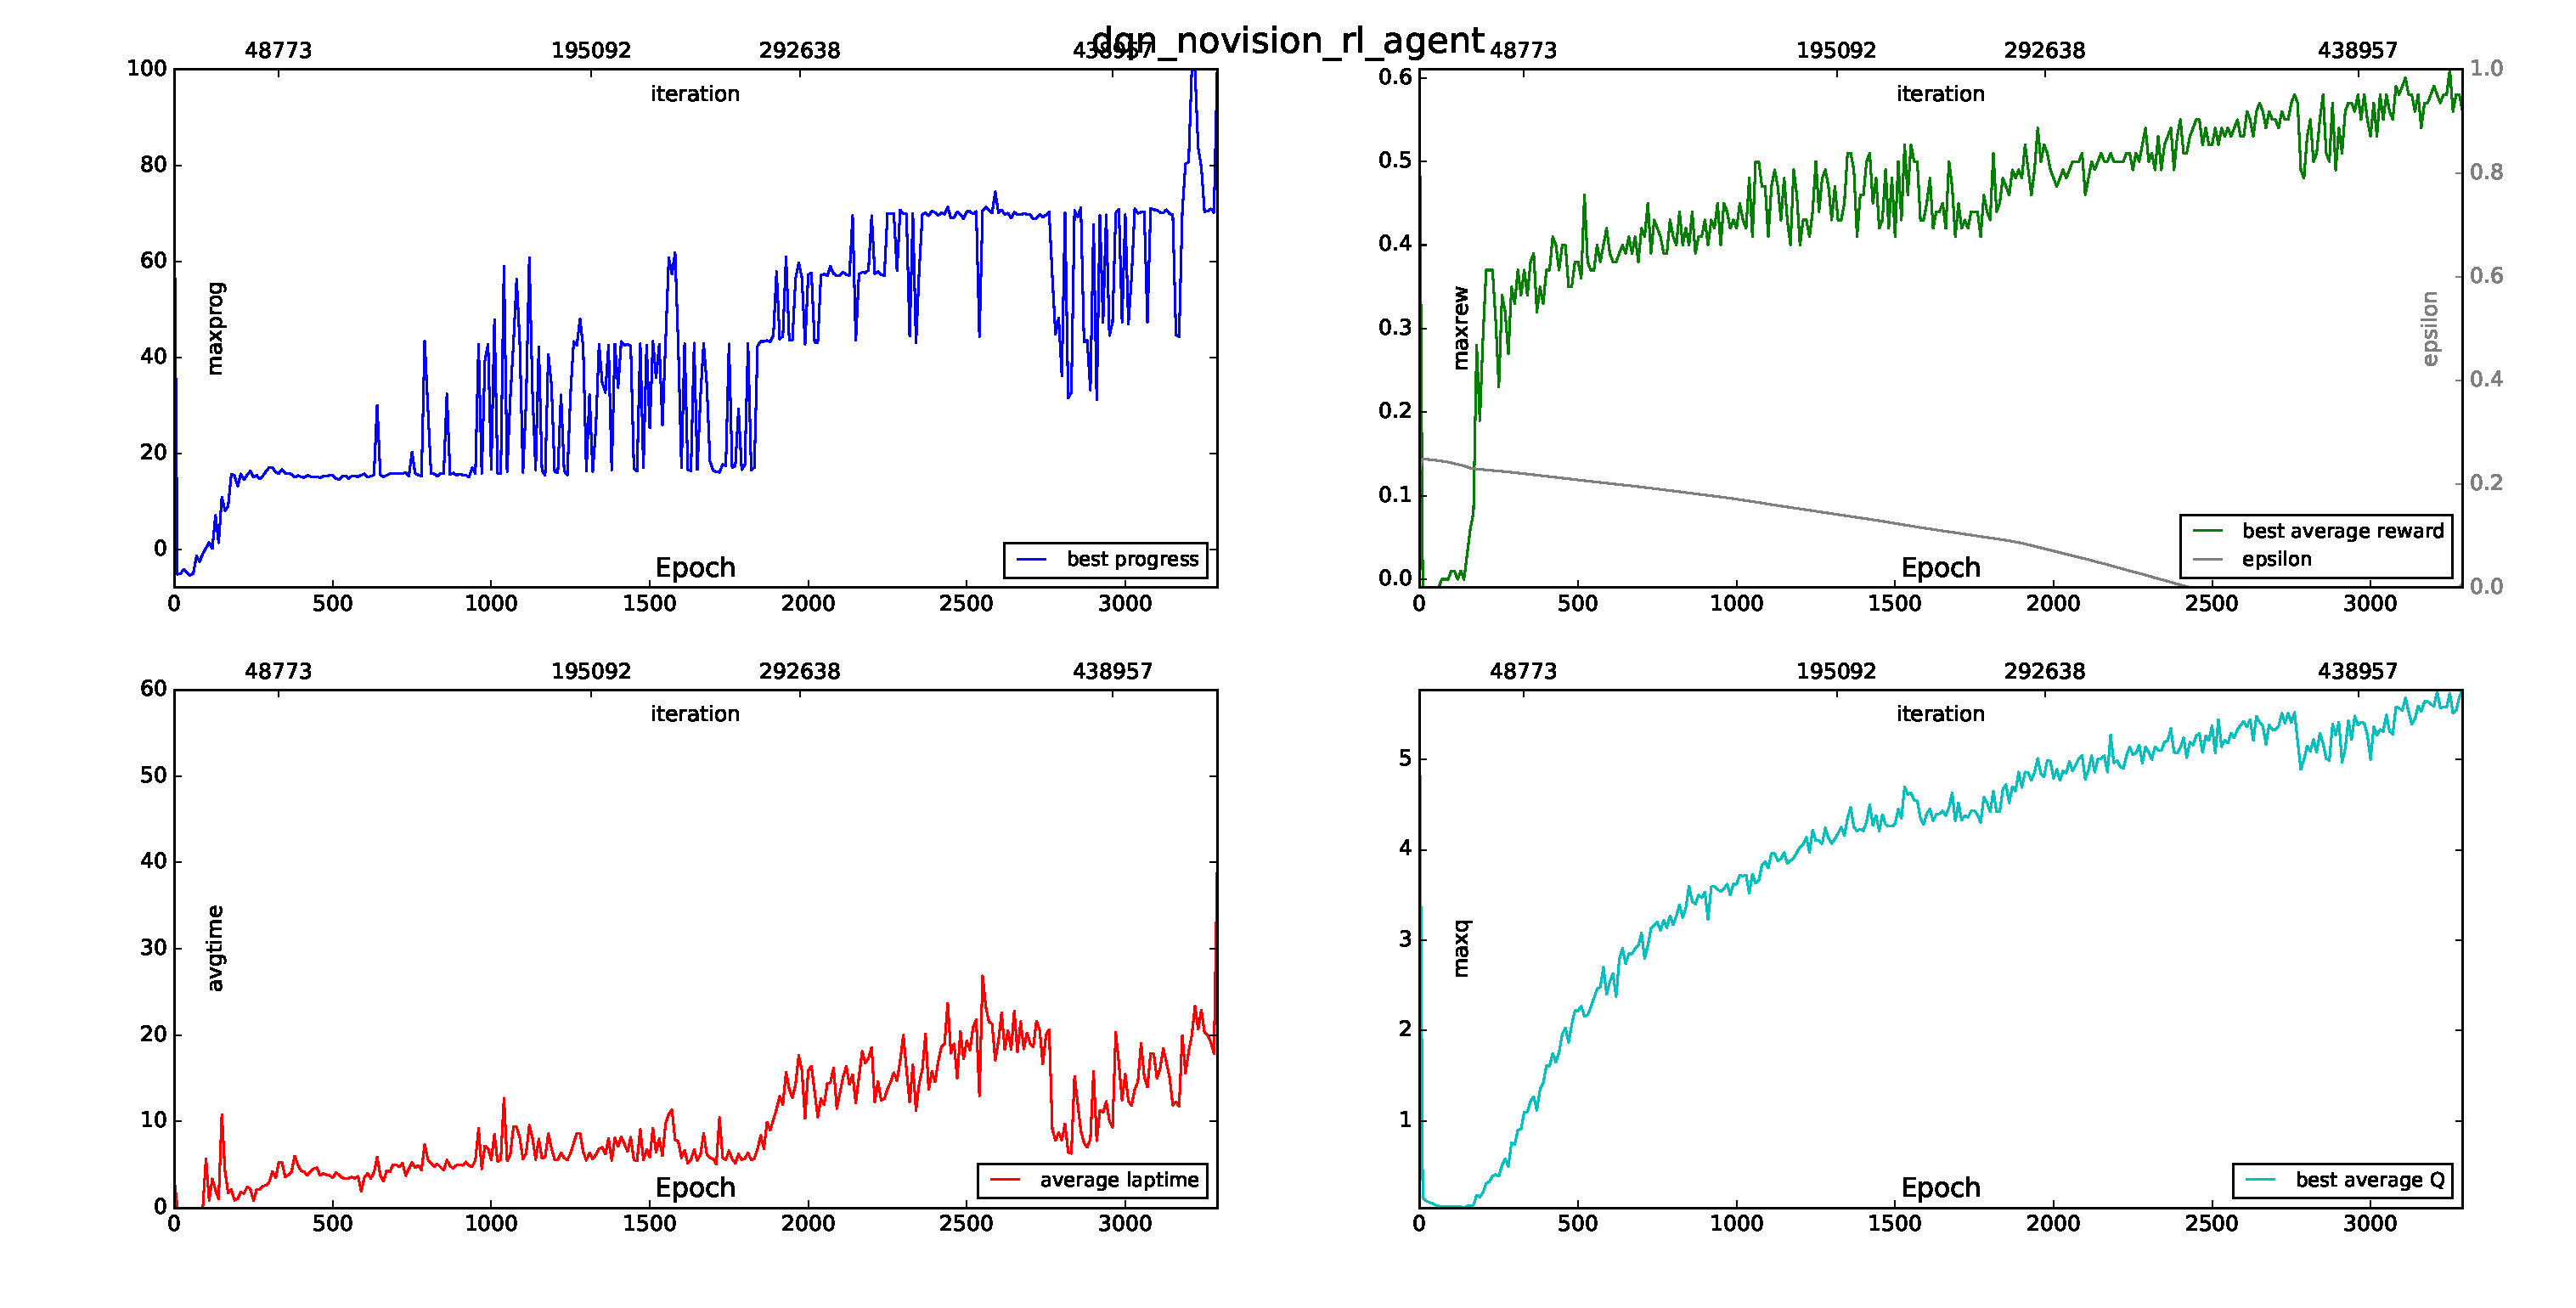
\includegraphics[trim={2.2cm 0cm 1cm 0cm},clip,width=\textwidth]{performance_plots/dqn_bestresult_meinreward_average10_3500ep}}%
	}%
	\centering
	\caption[Exemplary performance of the dqn\_novison\_rl\_agent]{Exemplary performance of the dqn\_novison\_rl\_agent. Plots are smoothed by averaging over 10 episodes.}
	\label{fig:dqn_result}
\end{figure}


In both cases, the Q-value, average reward and progress increases throughout training. Both agents are further able to complete a whole lap. To do so, DQN-agent required however around 3000 training episodes (over 400.000 minibatch-trainingsteps), whereas the DDPG-agent needed only around 1400 episodes (corresponding to less than 300.000 inferences). It is further interesting, the DQN-agent seems to learn incrementally, where each turn requires hundreds of training-iterations until it is mastered. In contrast to that, the DDPG-agent seems to generalize better from the first part of the track towards the whole track, as can be seen in the very steep learning curve towards the end.

\begin{figure}[h!]
	{%
		\setlength{\fboxsep}{0pt}%
		\setlength{\fboxrule}{1pt}%
		\fbox{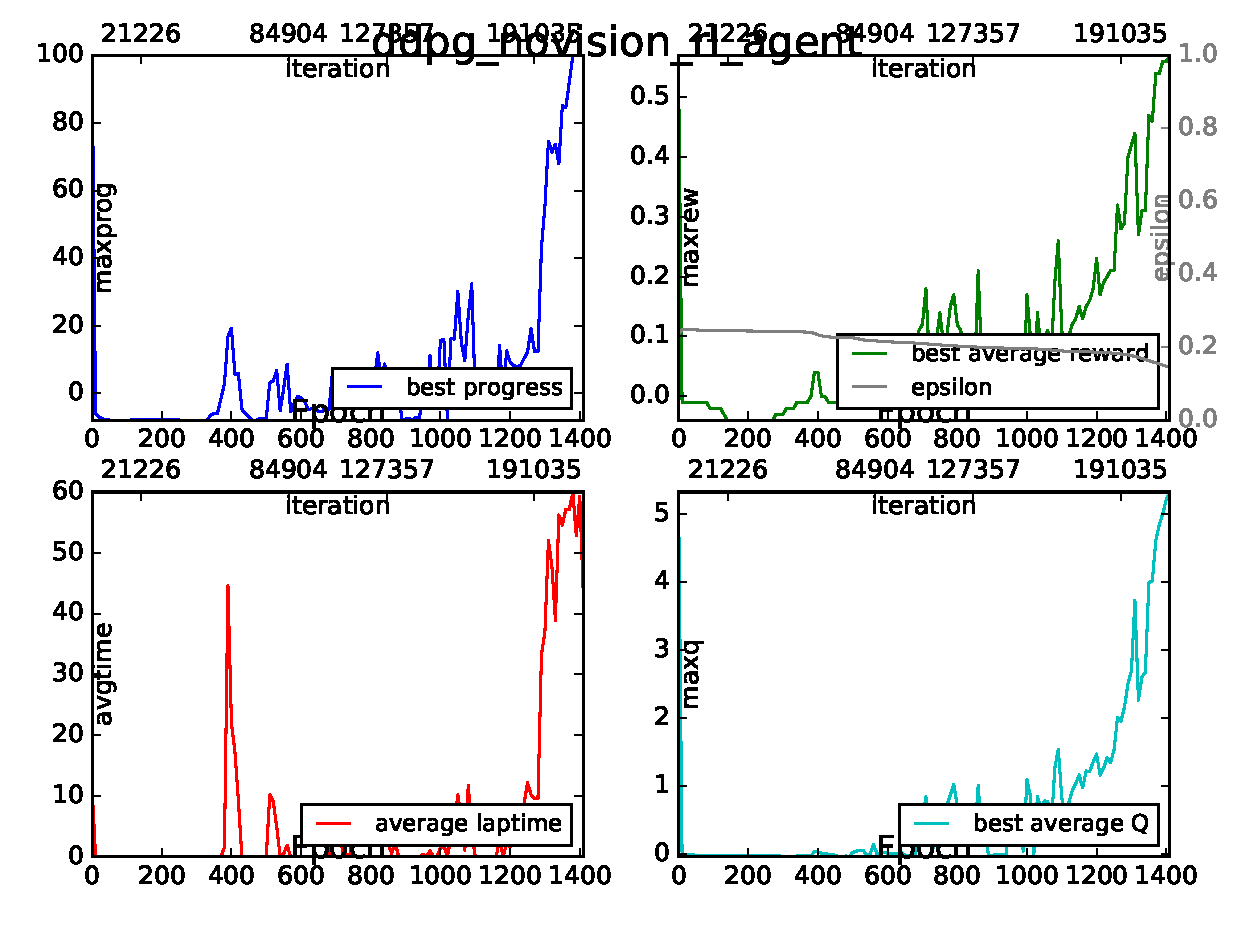
\includegraphics[width=.9\textwidth]{performance_plots/ddpg_bestresult_meinreward_average10_1400ep}}%
	}%
	\centering
	\caption[Exemplary performance of the ddpg\_novison\_rl\_agent]{Exemplary performance of the ddpg\_novison\_rl\_agent. Plots are smoothed by averaging over 10 episodes.}
	\label{fig:ddpg_result}
\end{figure}


This result shows that while an agent that discretizes the action-space can certainly learn the track, an agent that does so seems to learn slower than its continuous counterpart. As the continuous agent however also used a better exploration function, it is an open question how much of this performance gain must be accredited to that. 

Another question that remains open is, how much faster the laps driven by a continuous agent are will ultimately be. No full lap driven by either of the agents finished in less than $50$ seconds time, which is a lot more than the human average. As the action-space of continuous agents includes that of the discretized agents, it is certain that the upper limit of the former's maximal performance is least as high, and probably much higher, than that of the latter.

Interestingly, both algorithms oversteer a lot even in straight track sections, which leads to \textit{jittering} movement. This seems to be a general problem of the employed techniques, as it is seen throughout many other implementations\footnote{see for example this video \url{https://www.youtube.com/watch?v=4hoLGtnK_3U}, which is the performance of the implementation of the project \textit{DDPG-Keras-Torcs} as listed in table~\ref{tb:rlapproaches}.}.


\section{Incorporating pretraining}
\label{sec:incorporatePre}

One question this thesis aimed to answer is \textit{how to incorporate pretraining into reinforcedly learning agents}. As explained in section~\ref{sec:pretrainingcode}, an agent that trained supervisedly does not adequatly \keyword{transfer} this knowledge when applied to a reinforcement leaning paradigm. In this thesis, it was tried to find a solution for that by setting correct Q-values for the respective actions, while setting a Q-value of zero for all others.

To test if pretraining an agent increases the learning pace, an agent that performed q-pretraining as specified in section~\ref{sec:pretrainingcode} subsequently underwent normal reinforcement training. Specifically, a \term{ddpg\_novision\_rl\_agent} was pre-trained for $40.000$ pretraining steps on a dataset consisting of $46$ laps (around $14.000$ individual datapoints), such that it had a testing set performance of $96\%$. While the testing set accuracy is high, this agent barely got further than the first turn of the track.

Figure~\ref{fig:ddpg_incorpPre} shows the performance of this agent in actual reinforcement learning. As can be seen, while the rewards and q-values are high at the beginning, it seems impossible for the agent to use that knowledge. In fact, the graph rather suggests the opposite: 1) the reward drops very fast to zero, and stays close to zero for longer time than a non-pretrained agent, 2) the progress-milestone of $16\%$ is reached at around the same time than in an agent that did not perform pretraining (epoch 1300), and 3) The q-value is decreasing until this episode, rising only with the rise of the reward.

\begin{figure}[h]
	{%
		\setlength{\fboxsep}{0pt}%
		\setlength{\fboxrule}{1pt}%
		\fbox{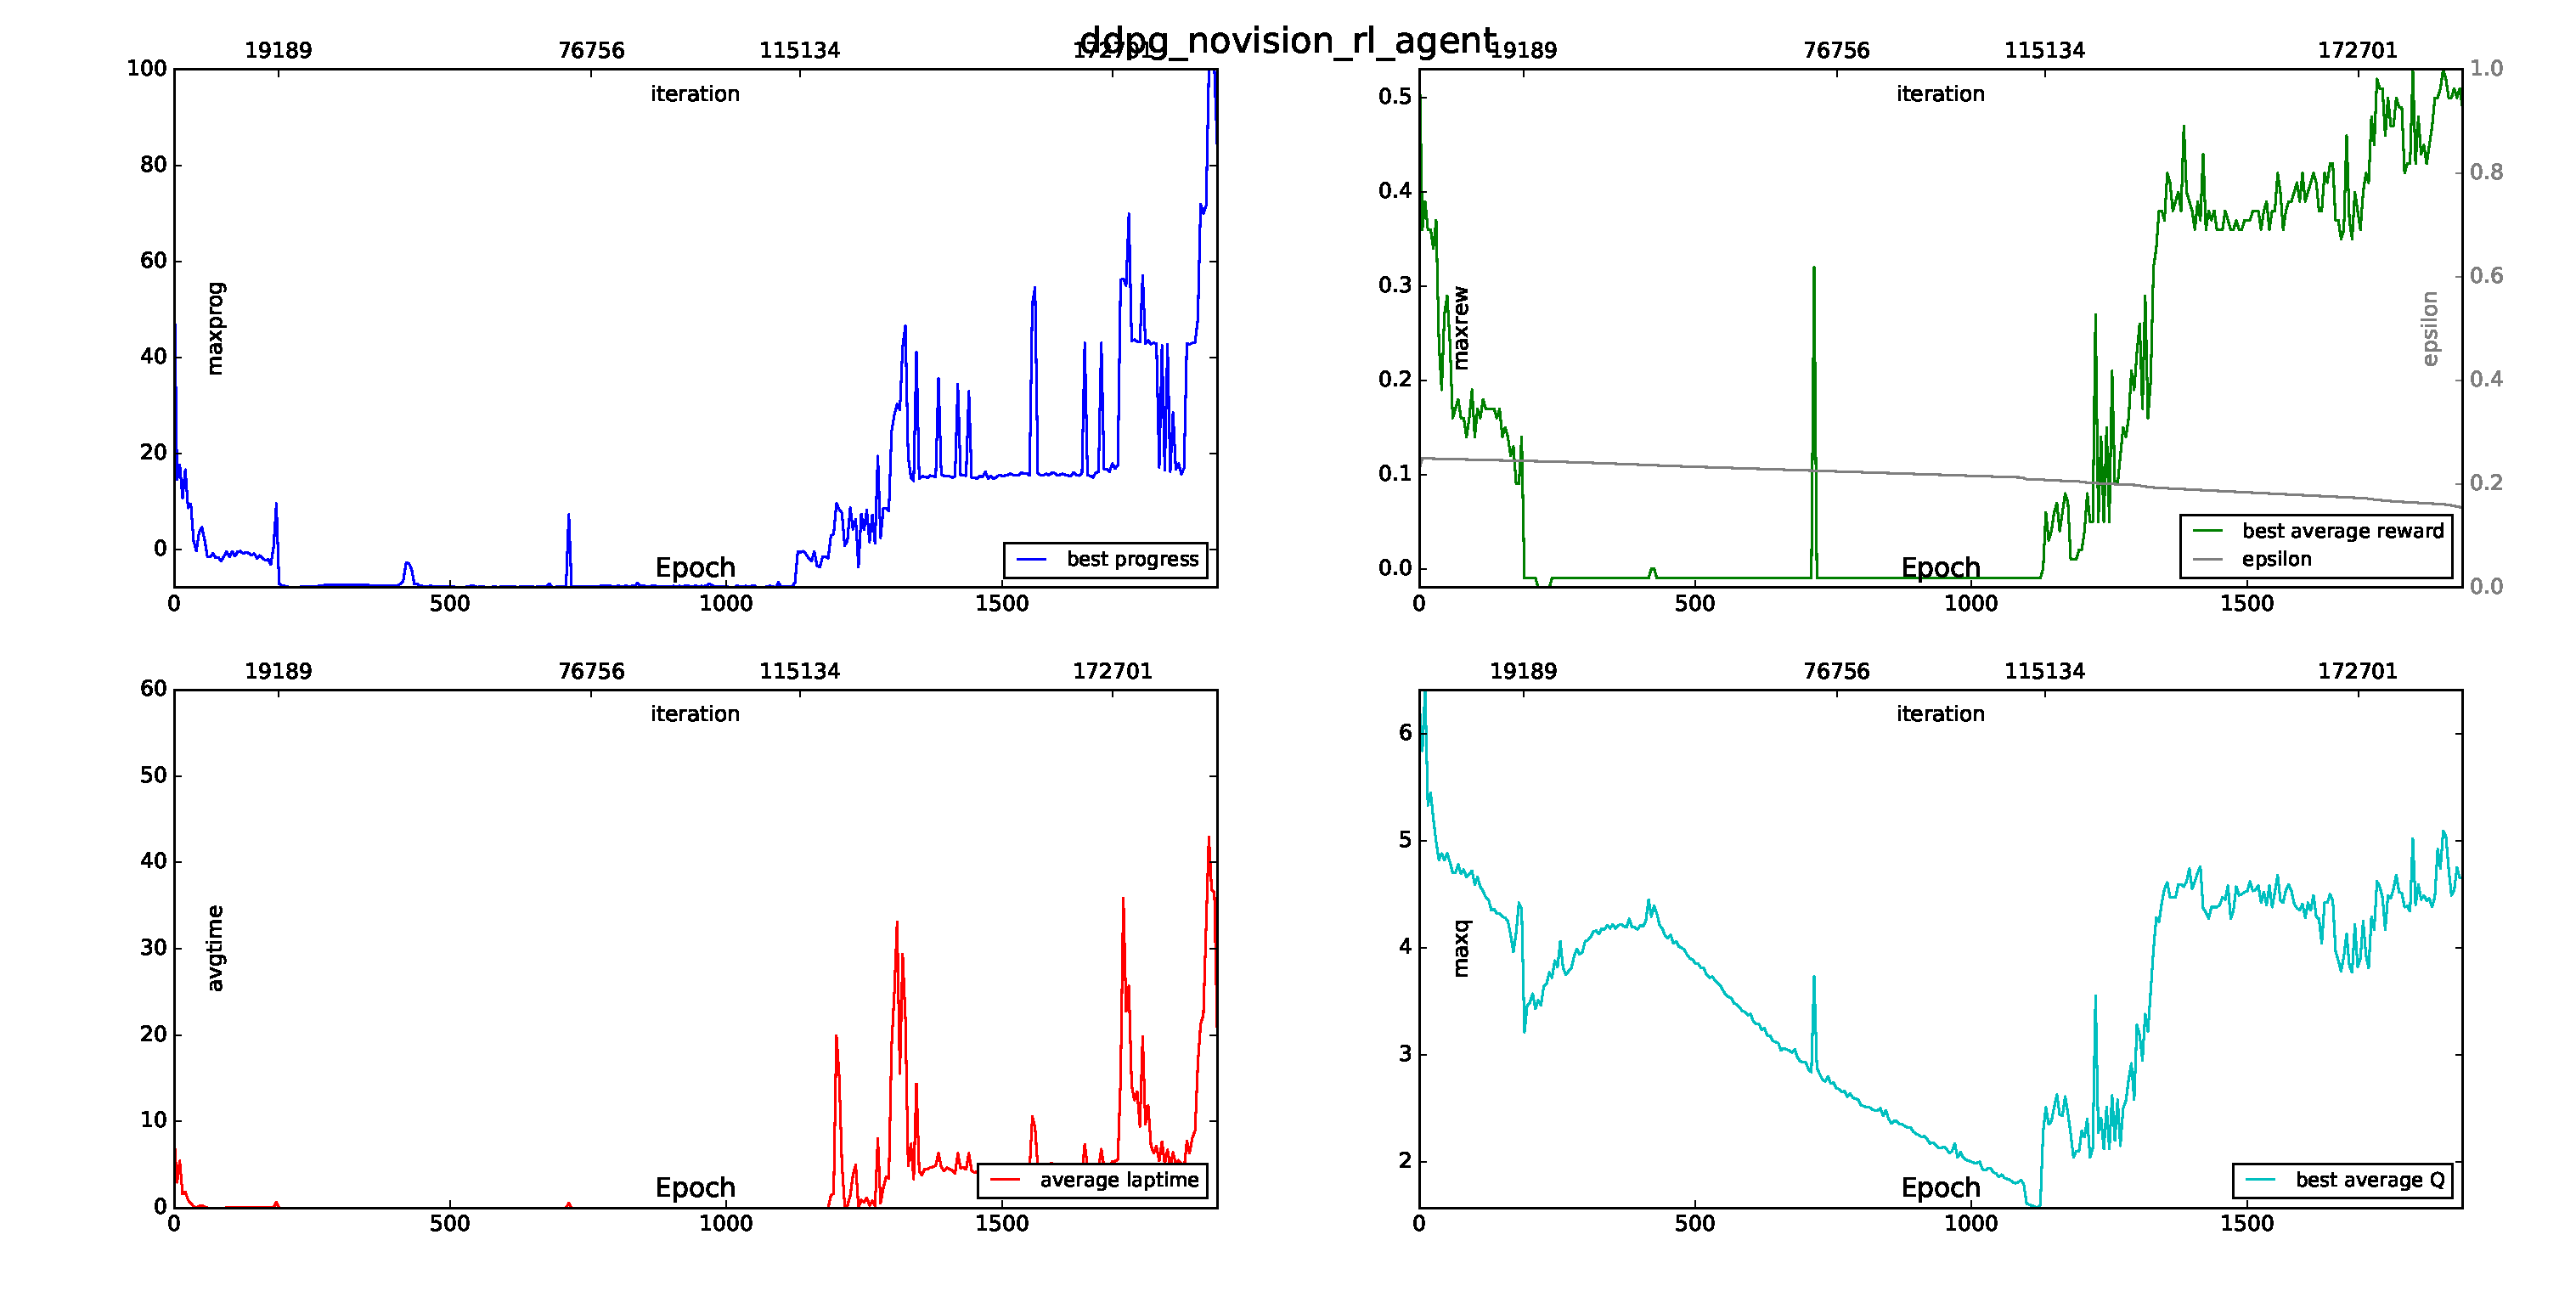
\includegraphics[trim={2.2cm 0cm 1cm 0cm},clip,width=\textwidth]{performance_plots/ddpg_meinward_average5_1900eps_2500pretrainepisodesauf17datasets}}%
	}%
	\centering
	\caption[Exemplary performance of the ddpg\_novison\_rl\_agent after 40000 pretrain steps]{Exemplary performance of the ddpg\_novison\_rl\_agent after 40000 pretraining steps. Plots are smoothed by averaging over 5 episodes.}
	\label{fig:ddpg_incorpPre}
\end{figure}

All in all, this agent completed its first full circuit after around 1900 episodes, more than 500 epochs later than an agent that did not perform pretraining. 

While not printed in this thesis, the plot of a pretrained \term{dqn\_novision\_rl\_agent} showed the same properties than the one described.

Concluding it must be said, that this thesis did not find a successful way to incorporate a pretraining based on manually driven rounds. This can be due to three main reasons: 1) the dataset was to small and must be extended, 2) it is simply not possible to learn from only \textit{good} rounds, or 3) the employed method is not the correct approach. Further resarch must be taken, especially trying to find a better method than the used one.

\section{Reward function}

One of the research questions asked \textit{what a good reward function looks like, that rewards the \textit{correct} behaviour at all times (including braking)}. All agents of the previously mentioned figures used the reward function from section~\ref{sec:reward}. The fact that these agents succeeded is evidence that incorporating this function contributes to successful driving policies. For this section, this method is compared with two other reward functions. 

\begin{figure}[h]
	{%
		\setlength{\fboxsep}{0pt}%
		\setlength{\fboxrule}{1pt}%
		\fbox{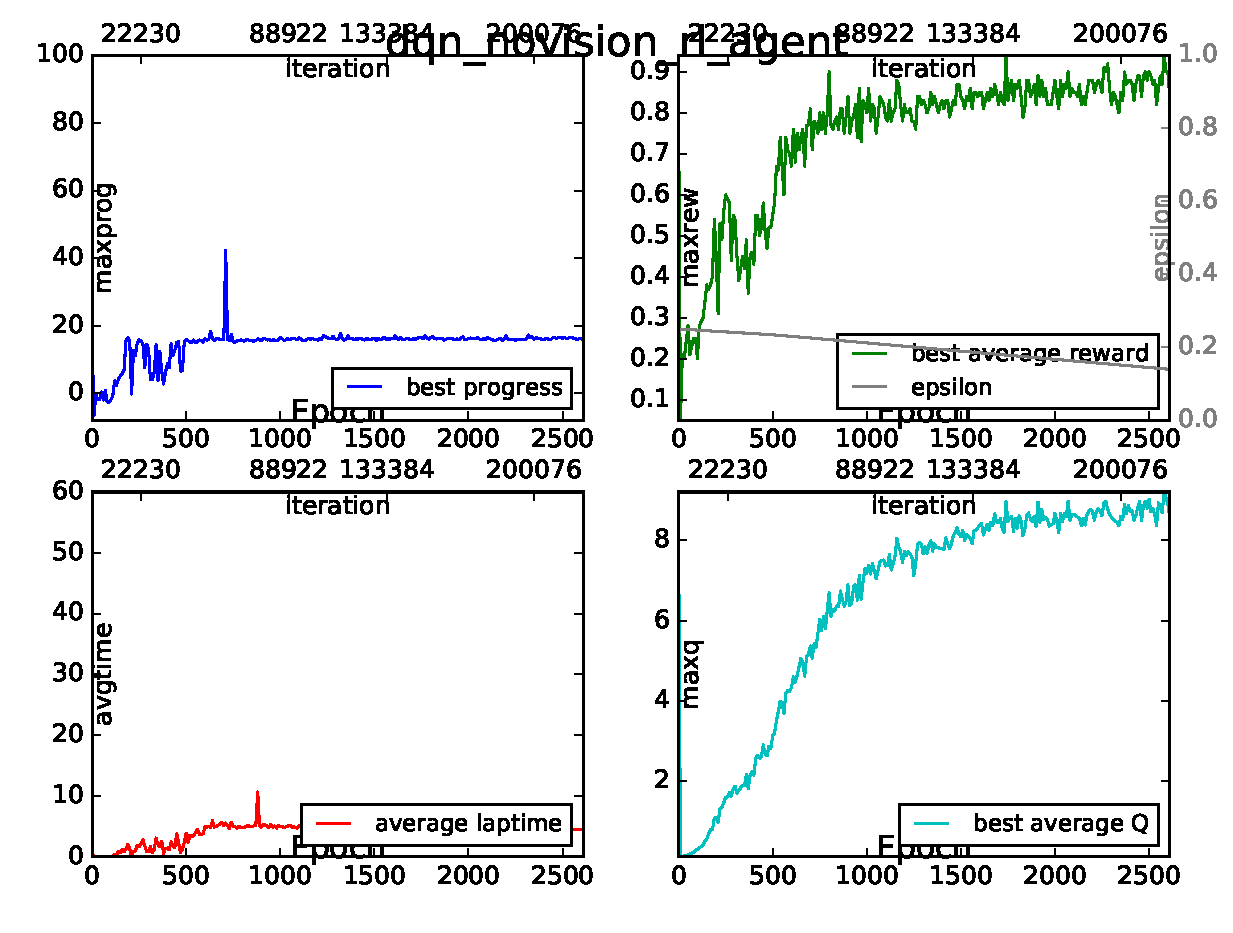
\includegraphics[width=.75\textwidth, height=.3\textheight ]{performance_plots/dqn_rewardspeed_smooth10_2600ep}}%
	}%
	\centering
	\caption[Exemplary performance of the dqn\_novison\_rl\_agent with the reward function from \cite{lillicrap_continuous_2015}]{Exemplary performance of the dqn\_novison\_rl\_agent with the reward function from \cite{lillicrap_continuous_2015}. Plots are smoothed by averaging over 10 episodes.}
	\label{fig:dqnrewardspeedstuff}
\end{figure}

In the original DDPG-Paper, the authors used as reward only \textit{the velocity of the car projected along the track direction and a penalty of -1 for collisions.}(quote \cite{lillicrap_continuous_2015}). In the given simulation, this corresponds to the feature \codeobj{SpeedSteer.SpeedInStreetDir}, with the collision punished in \codefunc{handle\_commands}. Figure~\ref{fig:dqnrewardspeedstuff} shows the performance of an agent that uses this reward function. 
As can be seen in the respective plot, this reward does not lead to successful results after $2500$ episodes, whereas the its average reward is almost maximal. As this reward function does not reward braking at all, the agent does not learn so and almost every episode ends with the car skidding at the first turn.

\begin{figure}[h]
	{%
		\setlength{\fboxsep}{0pt}%
		\setlength{\fboxrule}{1pt}%
		\fbox{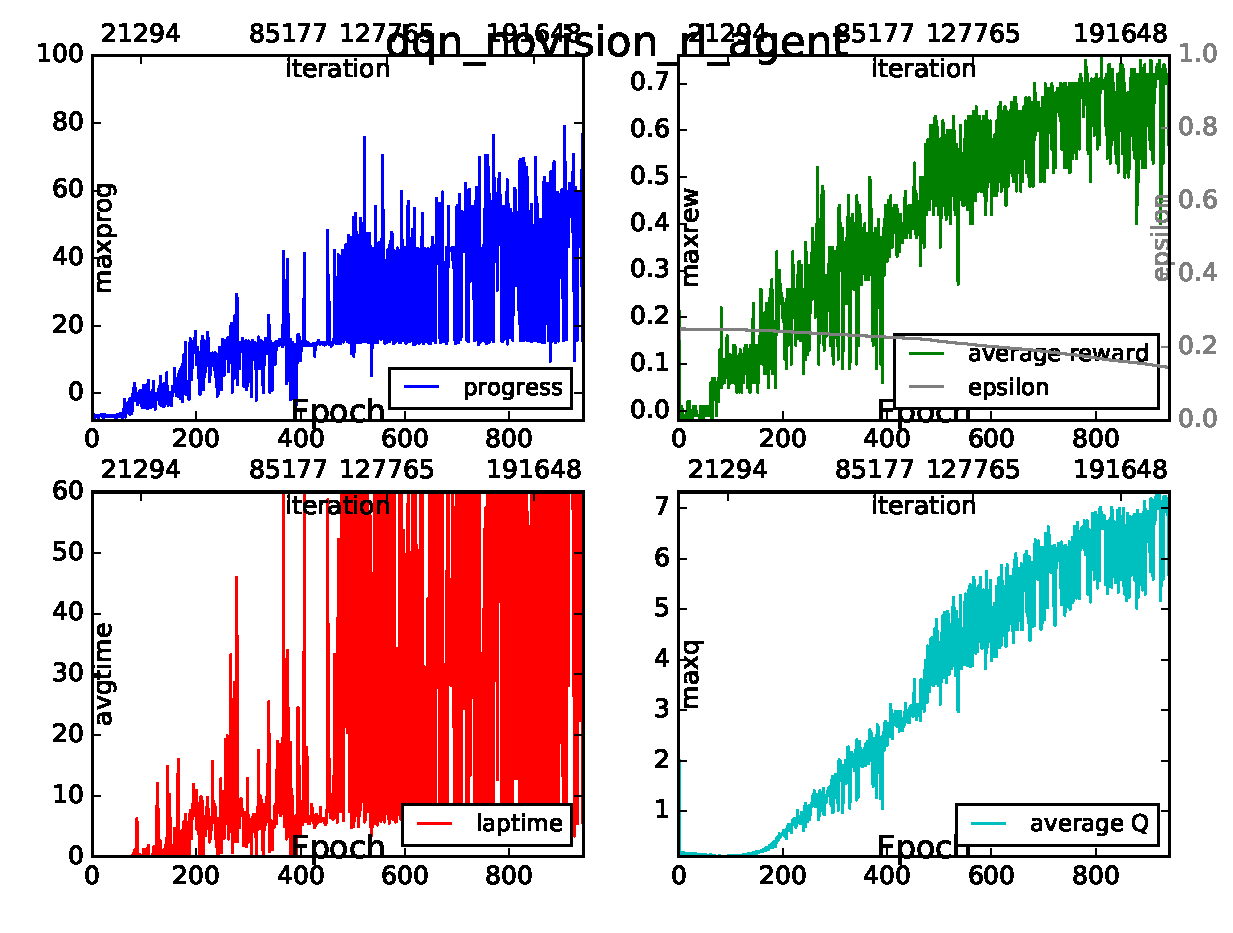
\includegraphics[width=.75\textwidth, height=.3\textheight]{performance_plots/dqn_rewardinrelationtowalldist_smooth1_900ep}}%
	}%
	\centering
	\caption[Exemplary performance of the dqn\_novison\_rl\_agent with SpeedInRelationToWallDist as only reward.]{Exemplary performance of the dqn\_novison\_rl\_agent with SpeedInRelationToWallDist as only reward. Plots are not smoothed.}
	\label{fig:dqnrewardinrelationtowall}
\end{figure}

To demonstrate the contributions of the other reward-components, figure~\ref{fig:dqnrewardinrelationtowall} shows the performance of an agent with the other reward-components removed (corresponding to lines 1-4 from algorithm~\ref{alg:speedinrelationto}). While the progress makes it appear that the agent learns a useful policy, the plot of the lap-time shows that almost every episode ended because of the time limitof 60 seconds. As this reward-function does always reward driving fast, it is no reasonable reward-function on its own. 
	
	%----------------------------------------------------------------------------------------
	%	THESIS CONTENT - APPENDICES
	%----------------------------------------------------------------------------------------
	
	\appendix % Cue to tell LaTeX that the following "chapters" are Appendices
	
	% Include the appendices of the thesis as separate files from the Appendices folder
	% Uncomment the lines as you write the Appendices
	
	% Appendix A

\newgeometry{
	a4paper,
	top=20mm,
	bottom=10mm,
	inner=24mm,
	outer=9mm,} %bindingoffset=.5cm

\lstset{
	numberblanklines=false
	,basicstyle=\ttfamily%
	,breaklines=true%
	,tabsize=1%
	,showstringspaces=false%
	,numbers=left%
	,numbersep=\lstnumbersep%
	,numberstyle=\lstnumberstyle%
	,framesep=0pt%
	,xleftmargin=\lstnumberwidth%
	,framexleftmargin=\lsthorizontalpadding%
	,xrightmargin=\lsthorizontalpadding%
	,framexrightmargin=\lsthorizontalpadding%
	,backgroundcolor=\color{verylightgray}%
	,postbreak=\ding{229}\space%
	,escapeinside={*(}{*)}
	\linespread{1.0}
}

\chapter{Comparison pseudocode \& Python-code} % Main appendix title
% https://tex.stackexchange.com/questions/22988/multicolumn-listing-for-comparison-in-latex

\label{AppendixA} % For referencing this appendix elsewhere, use \ref{AppendixA}

\vspace{-0.8cm}

\section{DQN}
\label{ap:dqn}

The following section describes the structure of an actual reinforcement learning agent, using a \textbf{Dueling Deep-Q-Network} as its model (as described in \cite{wang_dueling_2015}), performing \textbf{Double Q-learning} (as described in \cite{van_hasselt_deep_2015}). The last page consists of a comparison between the pseudocode of the general program flow of a DDQN-network (taken from \cite{mnih_human-level_2015}, with changes from \cite{van_hasselt_deep_2015} and \cite{lillicrap_continuous_2015} in blue) to the left and its corresponding python-code to the right, where each line of the pseudocode corresponds exactly to the respective line of the python-code. For information on which python- and tensorflow version are used, please see chapter~\ref{ch:program}. This code is extracted from the actual implementation within the scope of this thesis, with some changes abstracting away irrelevant details.\\

\lstinputlisting[language=Python, firstline=29]{codes/dqn.txt}
\begin{landscape}
	\begin{parcolumns}[distance=0.1em,colwidths={1=33em}]{2}
		\label{ap:dqn_comparison}
		\colchunk[1]{ \lstinputlisting[language=Pseudo]{codes/pseudo_dqn.txt}}
		\colchunk[2]{ \lstinputlisting[language=Python, lastline=27]{codes/dqn.txt} }
	\end{parcolumns}
\end{landscape}

\section{DDPG}
\label{ap:ddpg}

The following section describes the structure of an actual reinforcement learning agent, using an \textbf{actor-critic architecture} as its model, basing on the \text{Deep Deterministic Policy gradient}, as described in \cite{silver_deterministic_2014} and \cite{lillicrap_continuous_2015}. The last page consists of a comparison between the pseudocode of the general program flow of a DDPG-agent (taken from \cite{lillicrap_continuous_2015}) to the left and its corresponding python-code to the right, where each line of the pseudocode corresponds exactly to the respective line of the python-code. For information on which python- and tensorflow version are used, please see chapter+\ref{ch:program}. This code is extracted from the actual implementation within the scope of this thesis, with some changes abstracting away irrelevant details. Note that this listing does not contain a definition of a class \textit{agent}, as it is the same defined as in lines 1-48 of appendix~\ref{ap:dqn}.\\

\lstinputlisting[language=Python, firstline=33]{codes/ddpg.txt}
\begin{landscape}
	\begin{parcolumns}[distance=0.1em,colwidths={1=33em}]{2}
		\label{ap:ddpg_comparison}
		\colchunk[1]{ \lstinputlisting[language=Pseudo]{codes/pseudo_ddpg.txt}}
		\colchunk[2]{ \lstinputlisting[language=Python, lastline=32]{codes/ddpg.txt} }
	\end{parcolumns}
\end{landscape}




	\restoregeometry
	% Appendix B

\newgeometry{
	a4paper,
	top=20mm,
	bottom=10mm,
	inner=24mm,
	outer=9mm,} %bindingoffset=.5cm


\chapter{Screenshots of the game} % Main appendix title

\begin{figure}[h]
	\includegraphics[width=\textwidth]{screenshot_overview}
	\centering
	\caption{Start screen of the game, also showing a bird-eye view of the track}
	\label{fig:overviewshot}
\end{figure}

\begin{figure}[h]
	\includegraphics[width=\textwidth]{screenshot_human_juststarted}
	\centering
	\caption{\textbf{Drive} mode. For a description of the UI components, it is referred to section~\ref{ch:gamedescription}}
	\label{fig:humandriveshot}
\end{figure}

\begin{figure}[h]
	\includegraphics[width=\textwidth]{screenshot_driveAI}
	\centering
	\caption{\textbf{Drive AI} mode, showing many additional information directly on the screen. For a description of those, it is referred to sections~\ref{ch:gamedescription} and \ref{ch:thevectors}}
	\label{fig:aidriveshot}
\end{figure}

	\restoregeometry
	% Appendix C

\newgeometry{
	a4paper,
	top=20mm,
	bottom=10mm,
	inner=24mm,
	outer=9mm,} %bindingoffset=.5cm


\chapter{Informal description of the files belonging to the game} % Main appendix title

\label{AppendixC}


\renewcommand{\i}{$\bullet$~}
\renewcommand{\ni}{\\ \i}

\begin{landscape}
\begin{table}
	\resizebox{\linewidth}{!}{
		
		{\def\arraystretch{2}\tabcolsep=10pt
			\begin{tabular}{l|l|l|l|l|l|l|l}

Filename & attached to & knows & Start() & Update() & FixedUpdate() & Other behaviour & other functions\\
\hline \hline
UIScript.cs & Object Hierachy & all UI components & enable drivingOverlayActive & \blap{\i DrivingOverlayHandling: update GUI while \inlinecode{driving} \ni MenuOverlayHandling: update GUI and listen for input while \inlinecode{menu}} & & onGUI(): Print Debug Information on screen & \\[2\ucht]
\hline
Gamescript.cs & Object Hierachy & & \blap{\i Sets MiniMapCamera distances \ni Sets \inlinecode{mode} to \inlinecode{menu}} & \blap{\i enable/disable \term{QuickPause} if other threads demand it \ni switch \inlinecode{mode} to \inlinecode{menu} on \keystroke{Esc}} & & & \blap{\i enabling and disabling QuickPause \ni SwitchMode inclusive the respective calls to initialize the mode}\\[2\ucht]
\hline
CarController.cs & Car & & Sets Car's position & \blap{\i Rotates and adjust height of visible wheels \ni Enable reverse gear on \keytroke{R}} & \blap{\i Sets Car's Forces to zero after a reset \ni handles friction, checks if lap invalid, applices forces to Car} & & \blap{\i ResetCar and ResetToPosition \ni AdjustFriction \ni GetSurface}\\[3\ucht]
\hline
TimingScript.cs & TimingSystem's Box Collider & & & & & OnTriggerExit(): \blap{\i sets fast- and lastlaptime \ni calls Recfinishlist and, if applicable, AiInt.EndRound \ni resets activeLap, increases lapcoutn, \dots \ni Starts new lap for Rec} & Other timing-related functions\\[5\ucht]
\hline
ConfirmColliderScript.cs & TimingSystem's Confirm Colider  & & & & & OnTriggerExit(): Calls Timing.flipCCPassed() & \\
\hline
Recorder 


			\end{tabular}%
		}		
	}
\end{table}
\end{landscape}


	\restoregeometry
	% Appendix D

\newgeometry{
	a4paper,
	top=20mm,
	bottom=10mm,
	inner=24mm,
	outer=9mm,} %bindingoffset=.5cm

\lstset{
	numberblanklines=false
	,basicstyle=\ttfamily%
	,breaklines=true%
	,tabsize=1%
	,showstringspaces=false%
	,numbers=left%
	,numbersep=\lstnumbersep%
	,numberstyle=\lstnumberstyle%
	,framesep=0pt%
	,xleftmargin=\lstnumberwidth%
	,framexleftmargin=\lsthorizontalpadding%
	,xrightmargin=\lsthorizontalpadding%
	,framexrightmargin=\lsthorizontalpadding%
	,backgroundcolor=\color{verylightgray}%
	,postbreak=\ding{229}\space%
	,escapeinside={*(}{*)}
	\linespread{1.0}
}

\chapter{A minimally viable agent} % Main appendix title
% https://tex.stackexchange.com/questions/22988/multicolumn-listing-for-comparison-in-latex

\label{AppendixD} % For referencing this appendix elsewhere, use \ref{AppendixA}

\begin{lstlisting}[language=Python, frame=none]
import tensorflow as tf
#====own classes====
from agent import AbstractRLAgent
from dddqn import DDDQN_model 



class Agent(AbstractRLAgent):    
def init(self, conf, containers, isPretrain=False, start_fresh=False, *args, **kwargs):
	self.name = "dqn_rl_agent"
	super().init(conf, containers, isPretrain, start_fresh, *args, **kwargs)
	self.ff_inputsize = conf.speed_neurons + conf.num_actions * conf.ff_stacksize #32
	self.model = DDDQN_model(self.conf, self, tf.Session(), isPretrain=isPretrain)
	self.model.initNet(load=("preTrain" if (self.isPretrain and not start_fresh) else (not start_fresh)))


def policyAction(self, agentState):
	action, _ = self.model.inference(self.makeInferenceUsable(agentState)) 
	throttle, brake, steer = self.dediscretize(action[0])
	toUse = "["+str(throttle)+", "+str(brake)+", "+str(steer)+"]"
	return toUse, (throttle, brake, steer)
\end{lstlisting}%


	\restoregeometry
		

	%----------------------------------------------------------------------------------------
	%	BIBLIOGRAPHY
	%----------------------------------------------------------------------------------------
	
	
	\printbibliography[heading=bibintoc]
	
	%----------------------------------------------------------------------------------------
	%	DECLARATION PAGE
	%----------------------------------------------------------------------------------------
	
	\begin{declaration}
		\addchaptertocentry{\authorshipname} % Add the declaration to the table of contents
		\noindent I, \authorname, hereby certify that the work presented here is, to the best of my knowledge and belief, original and the result of my own investigations, except as acknowledged, and has not been submitted, either in part or whole, for a degree at this or any other university.\\
		
		\vspace{10px}
		\noindent \rule[-0.3em]{25em}{0.5pt}\\ % This prints a line for the signature
		signature\\
		
		\vspace{4px}
		\noindent \rule[-0.3em]{25em}{0.5pt}\\ % This prints a line to write the date		
		city, date
		
%		\noindent I, \authorname, declare that this thesis titled, \enquote{\ttitle} and the work presented in it are my own. I confirm that:
%		
%		\begin{itemize} 
%			\item This work was done wholly or mainly while in candidature for a research degree at this University.
%			\item Where any part of this thesis has previously been submitted for a degree or any other qualification at this University or any other institution, this has been clearly stated.
%			\item Where I have consulted the published work of others, this is always clearly attributed.
%			\item Where I have quoted from the work of others, the source is always given. With the exception of such quotations, this thesis is entirely my own work.
%			\item I have acknowledged all main sources of help.
%			\item Where the thesis is based on work done by myself jointly with others, I have made clear exactly what was done by others and what I have contributed myself.\\
%		\end{itemize}
%		

	\end{declaration}
	
	\cleardoublepage
	
	%----------------------------------------------------------------------------------------
	
\end{document}  
